% ==============================================================================
\chapter{Thin sensors studies}
\label{ch:ThinSensorsStudies}
% ==============================================================================    

% The aim of the CLIC vertex detector is the precise determination of
% the displaced vertices and jet flavour-tagging in an environment with
% high occupancy from beam-induced backgrounds. Multi-layer barrel and
% endcap pixel detectors with geometrical coverage extending down to low
% polar angles ($\theta_{min}\sim8^{\circ}$) are foreseen to fulfill
% these requirements. The goal is to achieve a single-point resolution
% of $\sim 3\,\micron$ with $25\,\micron$ pixel pitch and analogue
% readout. A material budget of $\sim0.2\%$~X\textsubscript{0} per layer
% is required including readout, support and cabling. This can be
% achieved with $50\,\micron$ thick sensors on $50\,\micron$ thick
% readout ASICs.

As part of the R\&D programme for the CLIC vertex detector, the
performance of thin silicon sensors is quantified using the Timepix3
readout chip with $55\,\micron$ pixel pitch. $50\,\micron$ to
$150\,\micron$ thick planar sensors are bump-bonded to $700\,\micron$
thick Timepix3 ASICs and tested with particle beams.

The AllPix simulation framework (described in \cref{sec:AllPix}) is
used to simulate the performance of thin sensors and to understand the
charge sharing in such sensors. A digitiser is designed in AllPix
which simulates the sensor and the readout ASIC. Data are used to
validate the simulations. The simulation is finally extrapolated to
predict the spatial resolution for smaller pixels of $25\,\micron$
pitch which is aimed to be achieved for the CLIC vertex detector.

%% --------------------------------------------- %%
\section{Thin-sensor assemblies}
A list of Advacam planar n-in-p thin sensors ($50-150\,\micron$ thick)
bump-bonded to Timepix3 readout ASICs is shown in
\cref{tab:nominalBiasThreshold}. These assemblies are tested using the
CLICdp Timepix3 pixel-beam reference telescope at the CERN SPS with
the experimental setup as described in \cref{sec:CERN_SPS}.

\begin{table}[htbp]
  \centering
  \caption{Nominal operating bias voltage, threshold in DAC and
    calibrated in number of electrons (measured as described in
    \cref{sec:thresholdCalibration}) for the Advacam planar n-in-p
    assemblies bump bonded to Timepix3 ASICs.}
  \label{tab:nominalBiasThreshold}
  \begin{tabular}{lcccc}
    \toprule
    Timepix3 ID & Thickness [$\micron$] & Bias voltage [V] & Threshold [DAC] & Threshold [e\textsuperscript{-}]\\
    \midrule
    W19\_G7 & 50 & -15 & 1190 & $505\pm31$ \\
    W19\_F7 & 50 & -15 & 1187 & $566\pm33$ \\
    W19\_L8 & 50 & -15 & 1133 & $546\pm31$ \\
    W19\_C7 & 50 & -15 & 1148 & $571\pm34$\\ \hline
    W5\_E2 & 100 & -20 & 1160 & $537\pm33$ \\ \hline
    W5\_F1 & 150 & -30 & 1153 & $536\pm31$ \\ %%\hline
    %% W2\_J5 & 300 & 100 & 1170 & $565.7\pm1.6$ \\
    \bottomrule
  \end{tabular}
\end{table}

%% --------------------------------------------- %%
\subsection{Operating conditions}
\label{sec:operatingConditions}
The Timepix3 readout ASICs were operated with the optimised parameters
as described in \cref{tab:timepix3Operation}. The nominal values for
the threshold and the bias voltage are shown in
\cref{tab:nominalBiasThreshold}. For the nominal bias voltage, the
sensor is fully (or over) depleted. The nominal threshold set insures
that the readout chip is not operating under noisy conditions. The
error on the threshold is due to the threshold dispersion after the
chip equalisation. \cref{sec:operatingThreshold} describes the
procedure for the selection of the nominal threshold value. These
nominal values are held throughout the data taking except for the
cases where the threshold or the bias voltages are scanned.



% %% --------------------------------------------- %%
% \section{Samples and sensors geometries}
% %% The DAC settings used for the operation of the Timepix3 assemblies in
% %% test beams is summarised in \cref{tab:timepix3Operation}.
% %% \begin{itemize}
% %% \item I\textsubscript{krum} DAC is set to 10.
% %% \item TOT clock frequency: $40\,\megahertz$
% %% \item VFBK: 150
% %% \end{itemize}


% For most of the measurements, the DUT is perpendicular to the beam. A
% scan was done on the bias voltage and the threshold of the DUT. The
% bias scan allows to obtain the depletion voltage.

%% --------------------------------------------- %%

%% --------------------------------------------- %%
\section{Experimental and simulated results for thin sensors}

This section gives an overview on the performance of thin sensors. The
AllPix simulations of thin sensors are validated using test-beam data.


\subsection{Calibrated test beam data}
\label{sec:calibrated_test_beam_data}

The test pulse calibration as described in
\cref{sec:EnergyCalibration} is applied to the test beam data in order
to convert the TOT values into energy deposited by the MIP particles
in units of the number of electrons generated.


\cref{sec:testBeamDataCalibrated_TOT} shows the TOT distribution for
one, two, three and four-pixel clusters. The most-probable-value (MPV)
of the TOT distributions for different cluster sizes do not fully
align due to the non-linear behaviour of the Timepix3, as sharing the
same deposited charge amongst several pixels results in each pixel
having a higher TOT than would be expected from simply scaling the
charge. The calibrated energy distribution aligns for different
cluster sizes since the calibration takes into account the
non-linearities of the chip as shown in
\cref{sec:testBeamDataCalibrated_Edep}. For the $50\,\micron$ thick
sensor, the calibrated distributions do not align since higher
deposited energies tend to give higher cluster sizes and the
distributions for larger cluster sizes are biased towards larger
energy depositions.

\begin{figure}[htbp] \centering
  \begin{subfigure}[b]{0.3\textwidth}
    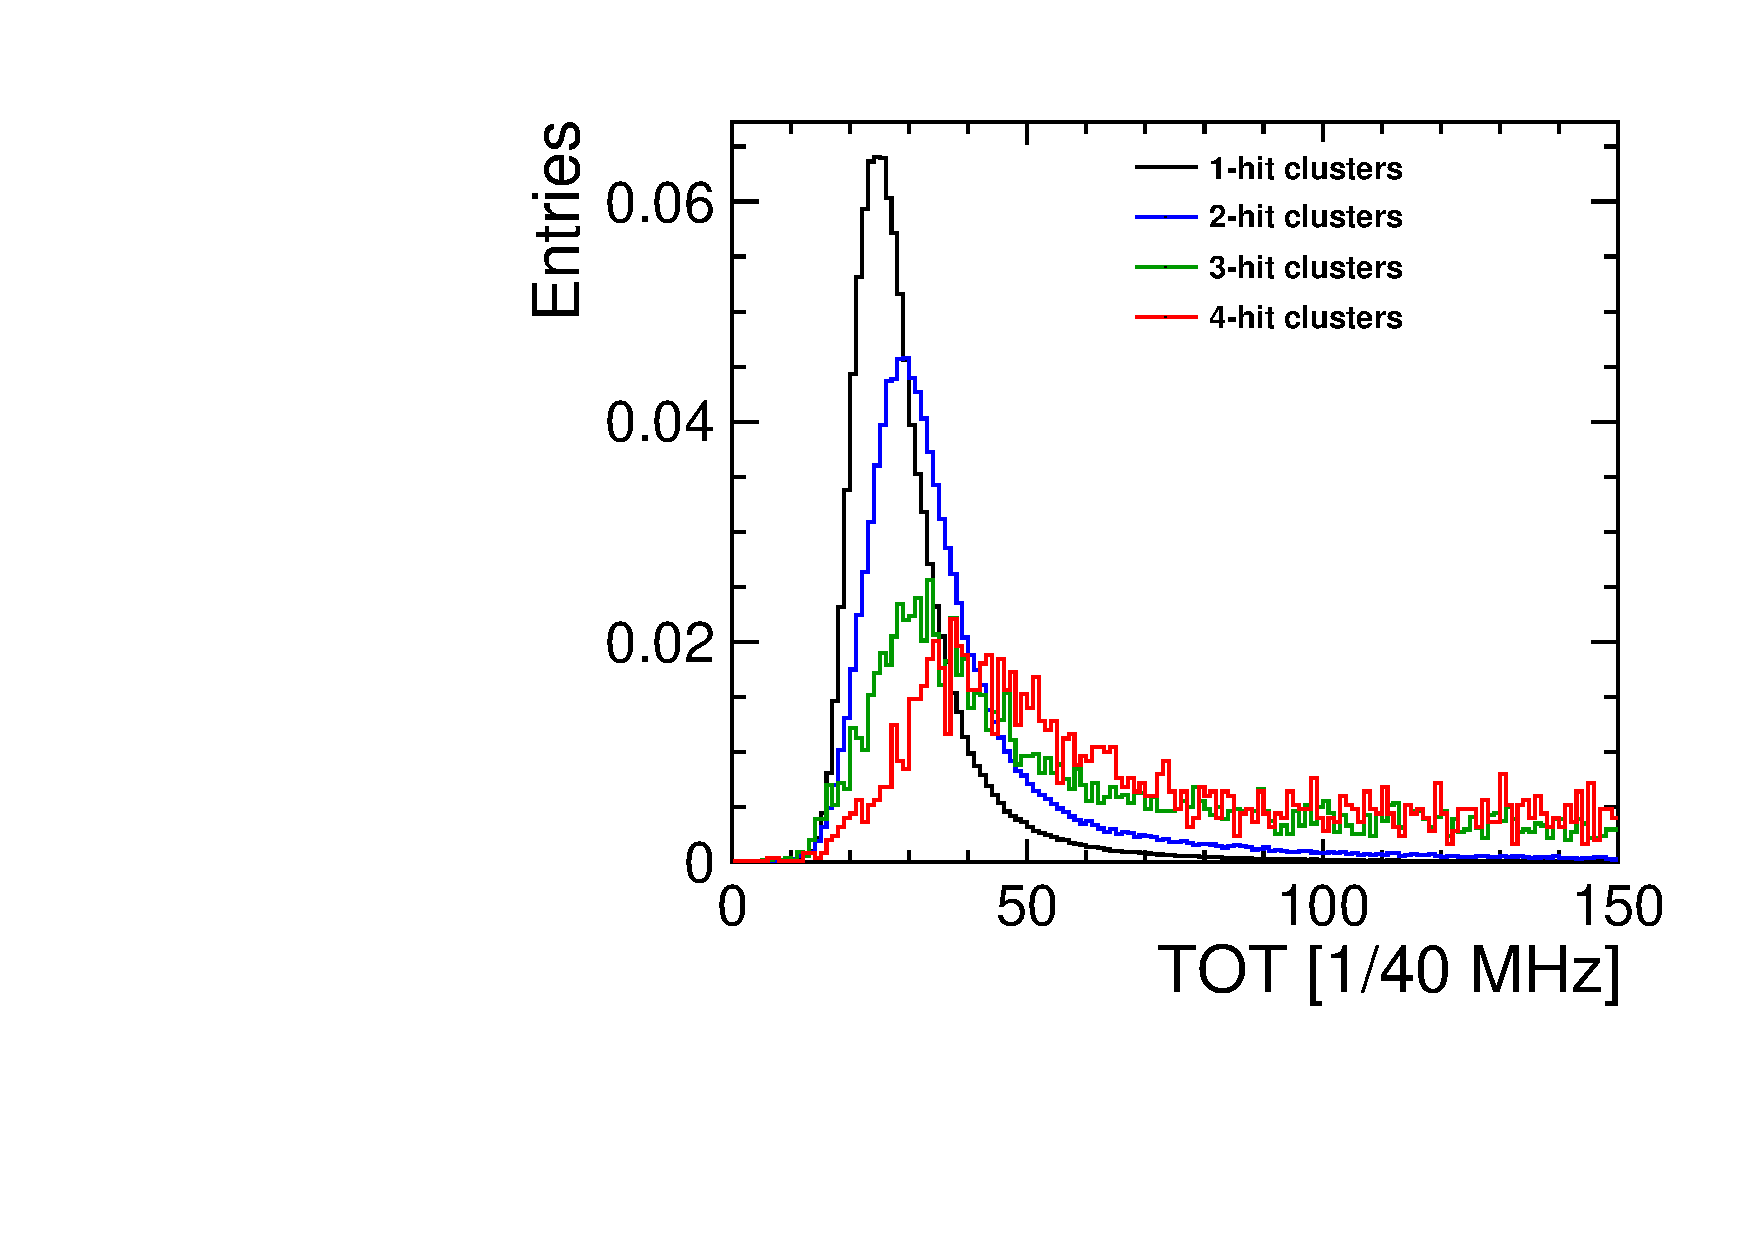
\includegraphics[width=\textwidth]{./figures/Calibration/TOT_Clusters_W0019_C07.pdf}
    \caption{W19\_C7}
  \end{subfigure} \hfill
  \begin{subfigure}[b]{0.3\textwidth}
    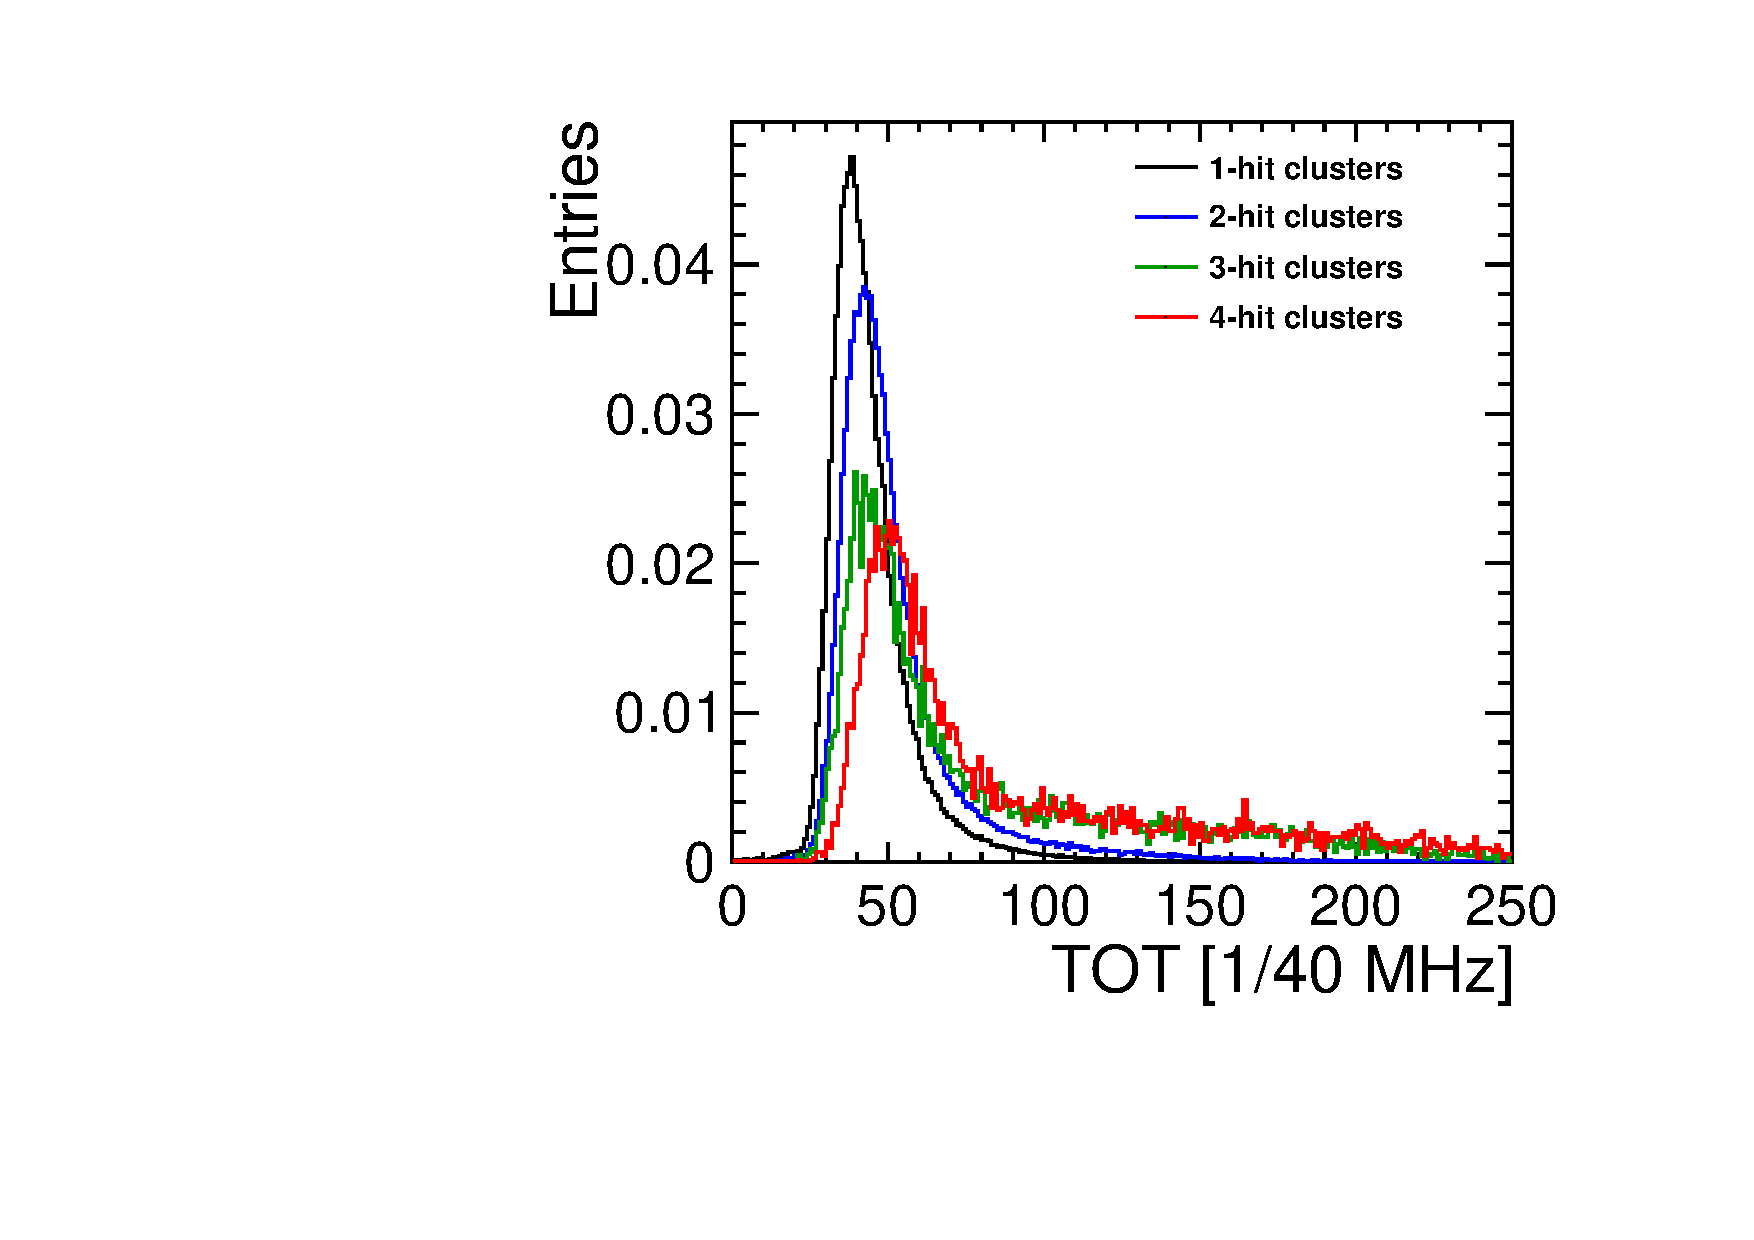
\includegraphics[width=\textwidth]{./figures/Calibration/TOT_Clusters_W0005_E02.pdf}
    \caption{W5\_E2}
  \end{subfigure}\hfill
  \begin{subfigure}[b]{0.3\textwidth}
    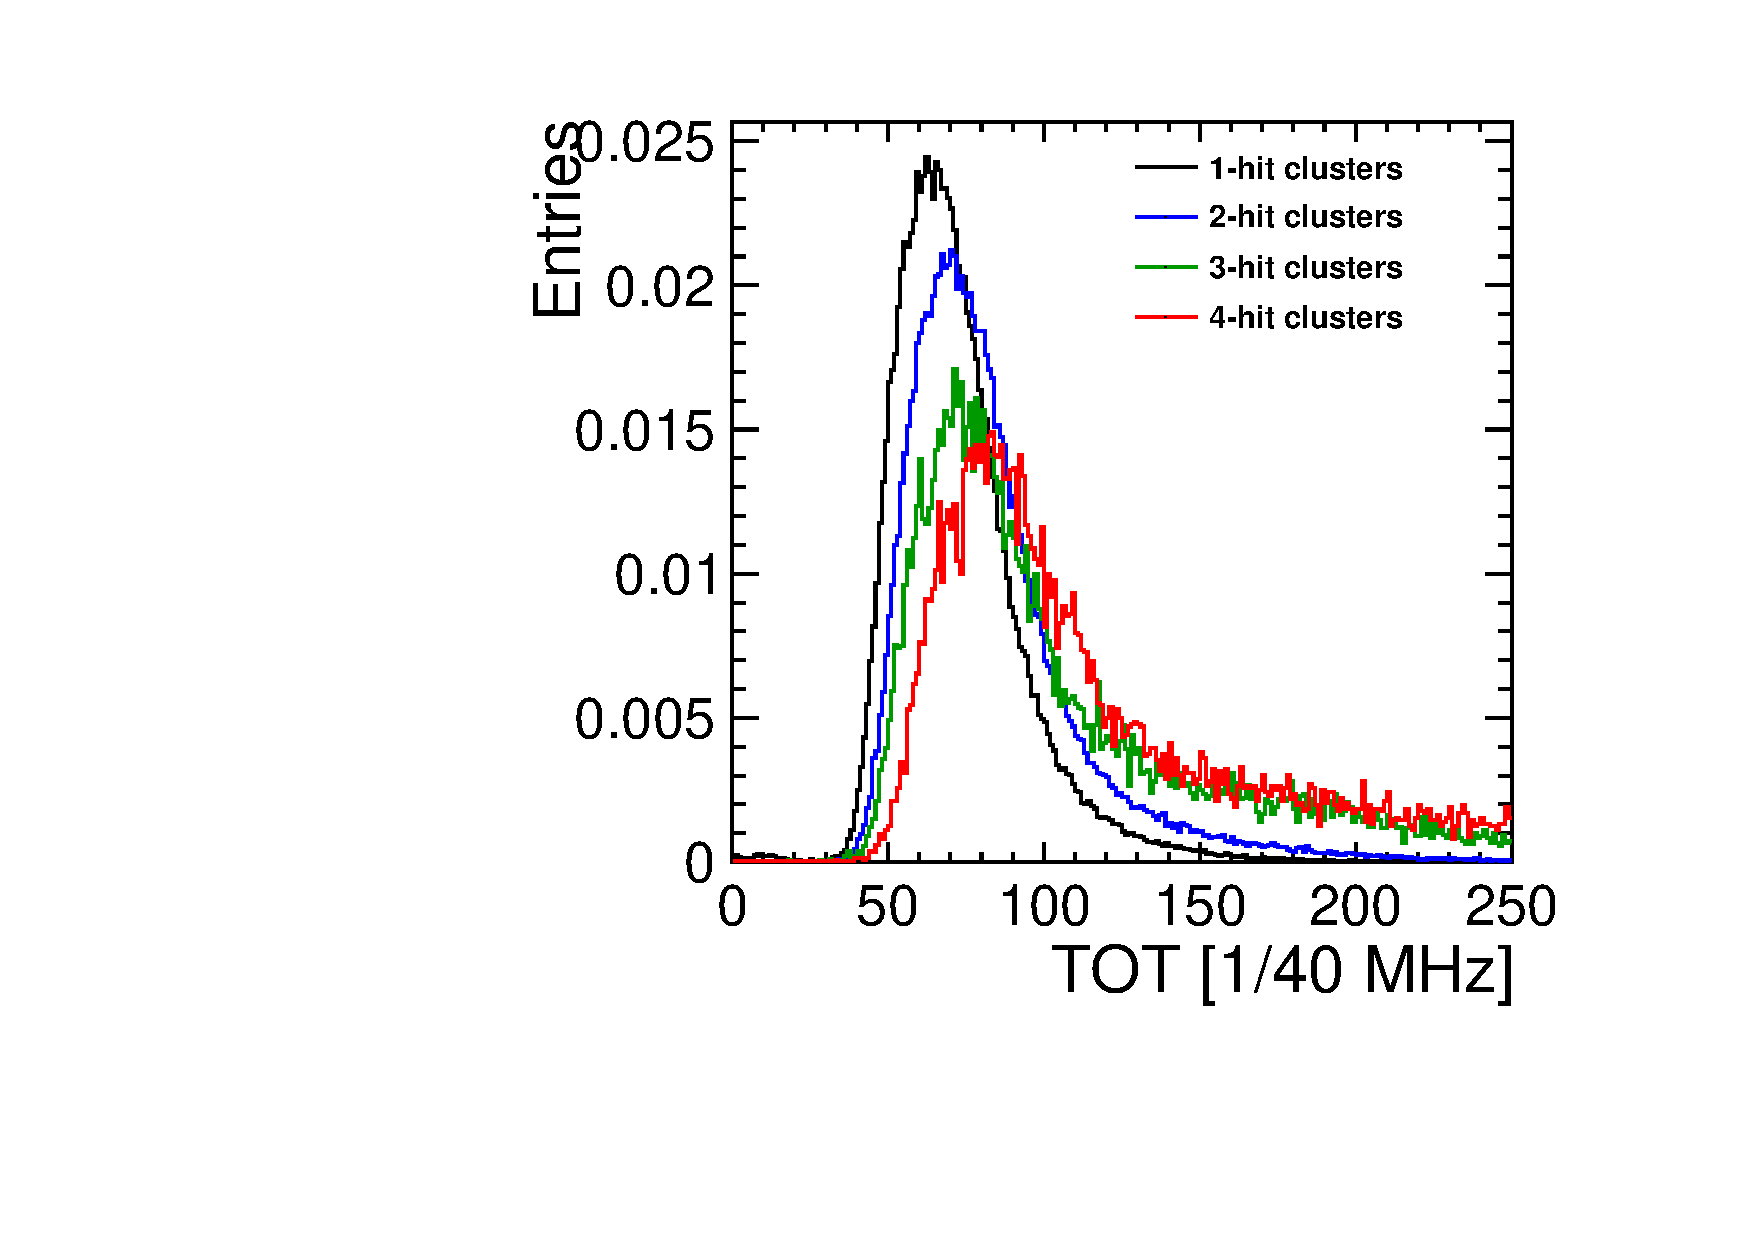
\includegraphics[width=\textwidth]{./figures/Calibration/TOT_Clusters_W0005_F01.pdf}
    \caption{W5\_F1}
  \end{subfigure}
  \caption{TOT distribution for one, two, three and four-pixel
    clusters for assemblies with (a) $50\,\micron$, (b) $100\,\micron$
    and (c) $150\,\micron$ thick planar sensors.}
  \label{sec:testBeamDataCalibrated_TOT}
\end{figure}

\begin{figure}[htbp] \centering
  \begin{subfigure}[b]{0.3\textwidth}
    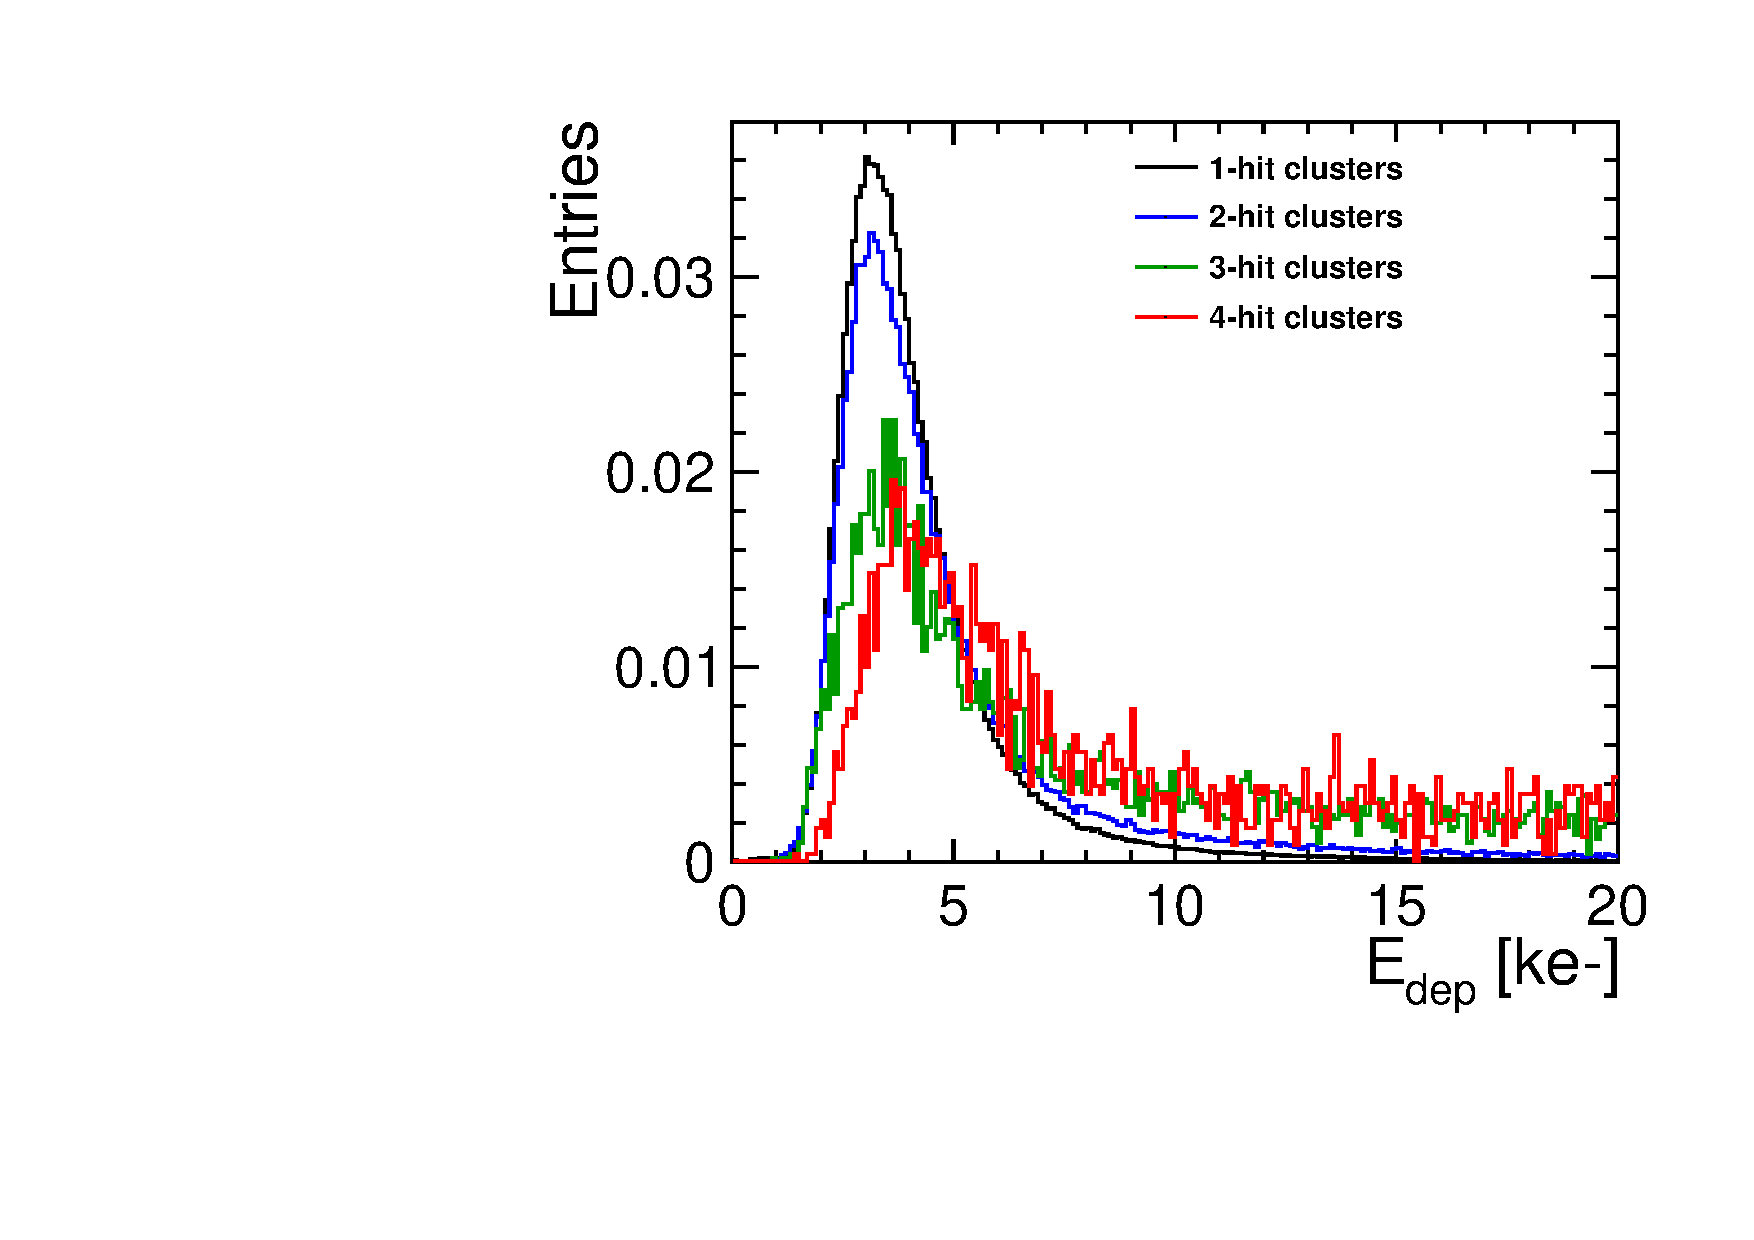
\includegraphics[width=\textwidth]{./figures/Calibration/Edep_Clusters_W0019_C07.pdf}
    \caption{W19\_C7}
  \end{subfigure} \hfill
  \begin{subfigure}[b]{0.3\textwidth}
    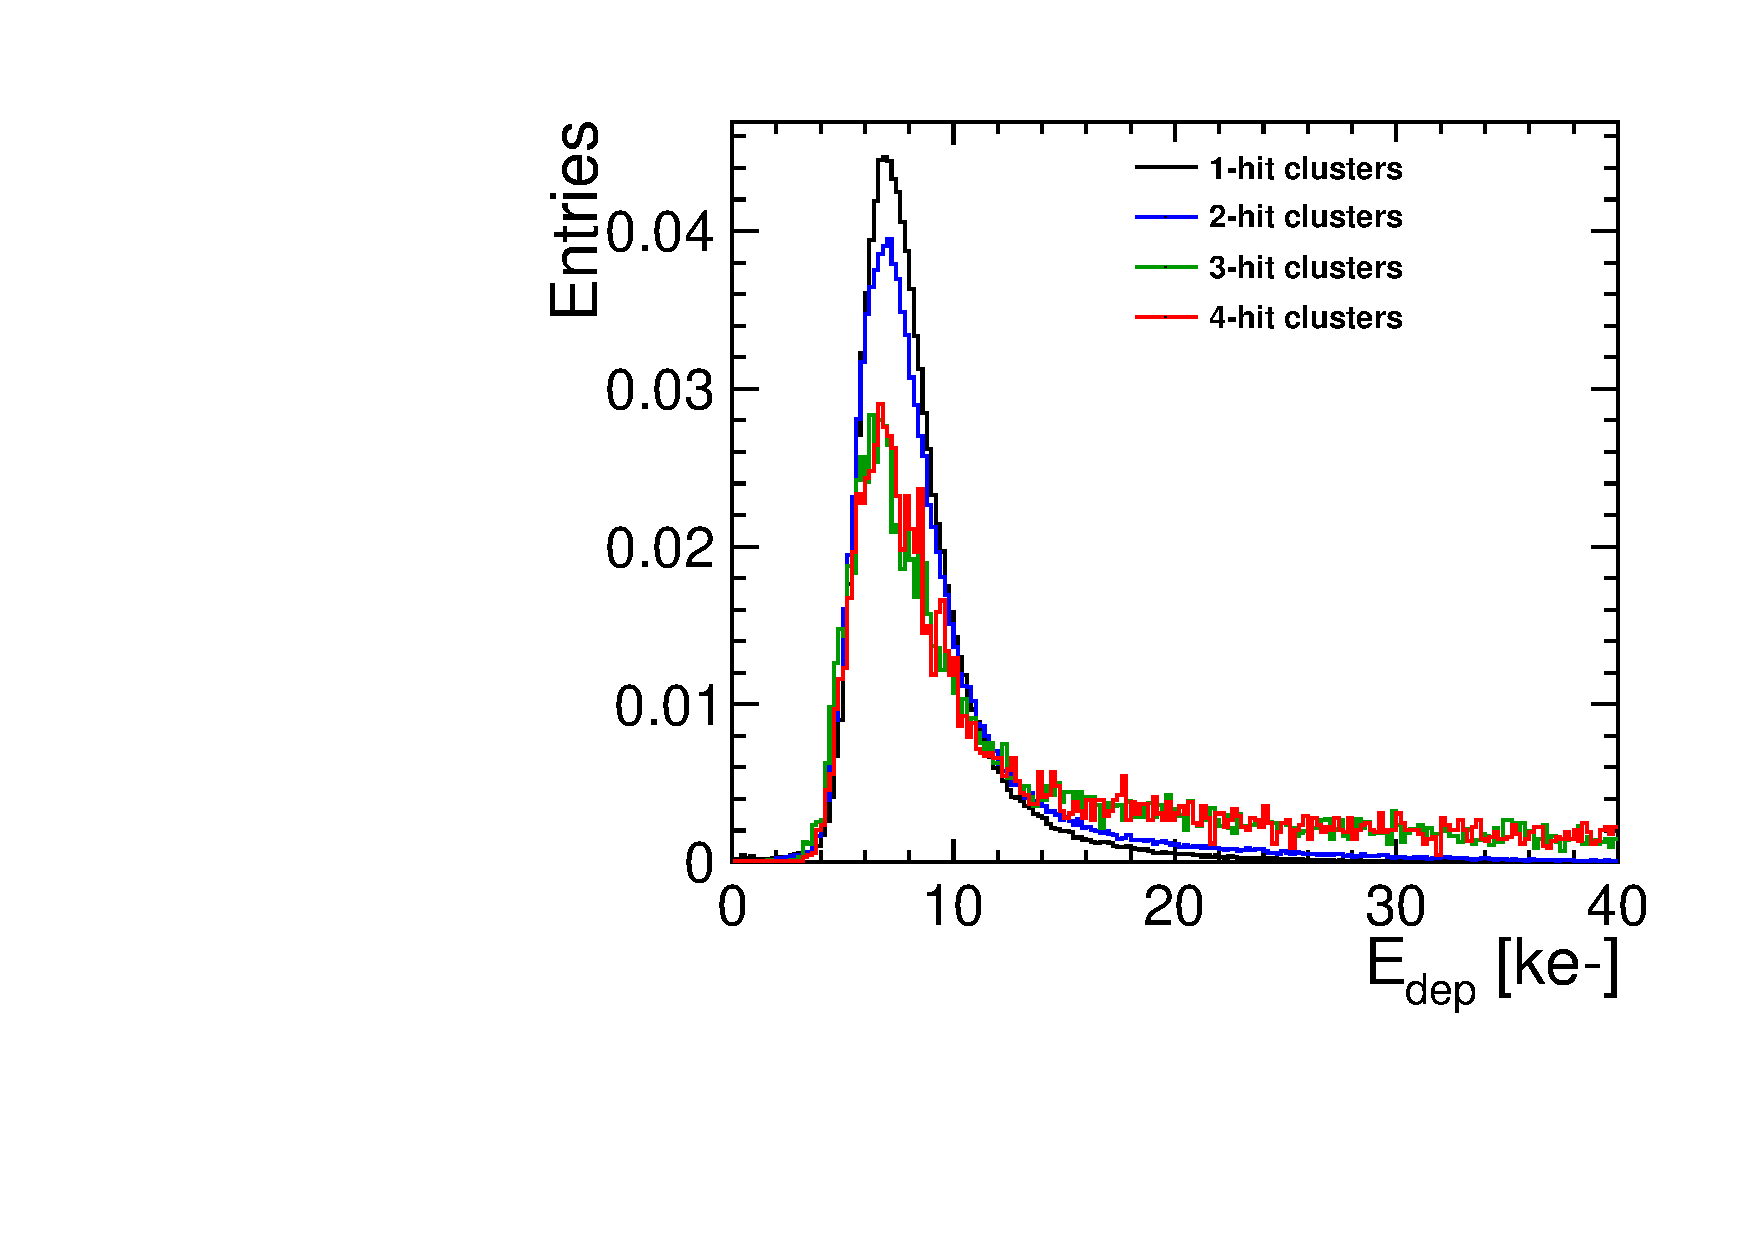
\includegraphics[width=\textwidth]{./figures/Calibration/Edep_Clusters_W0005_E02.pdf}
    \caption{W5\_E2}
  \end{subfigure}\hfill
  \begin{subfigure}[b]{0.3\textwidth}
    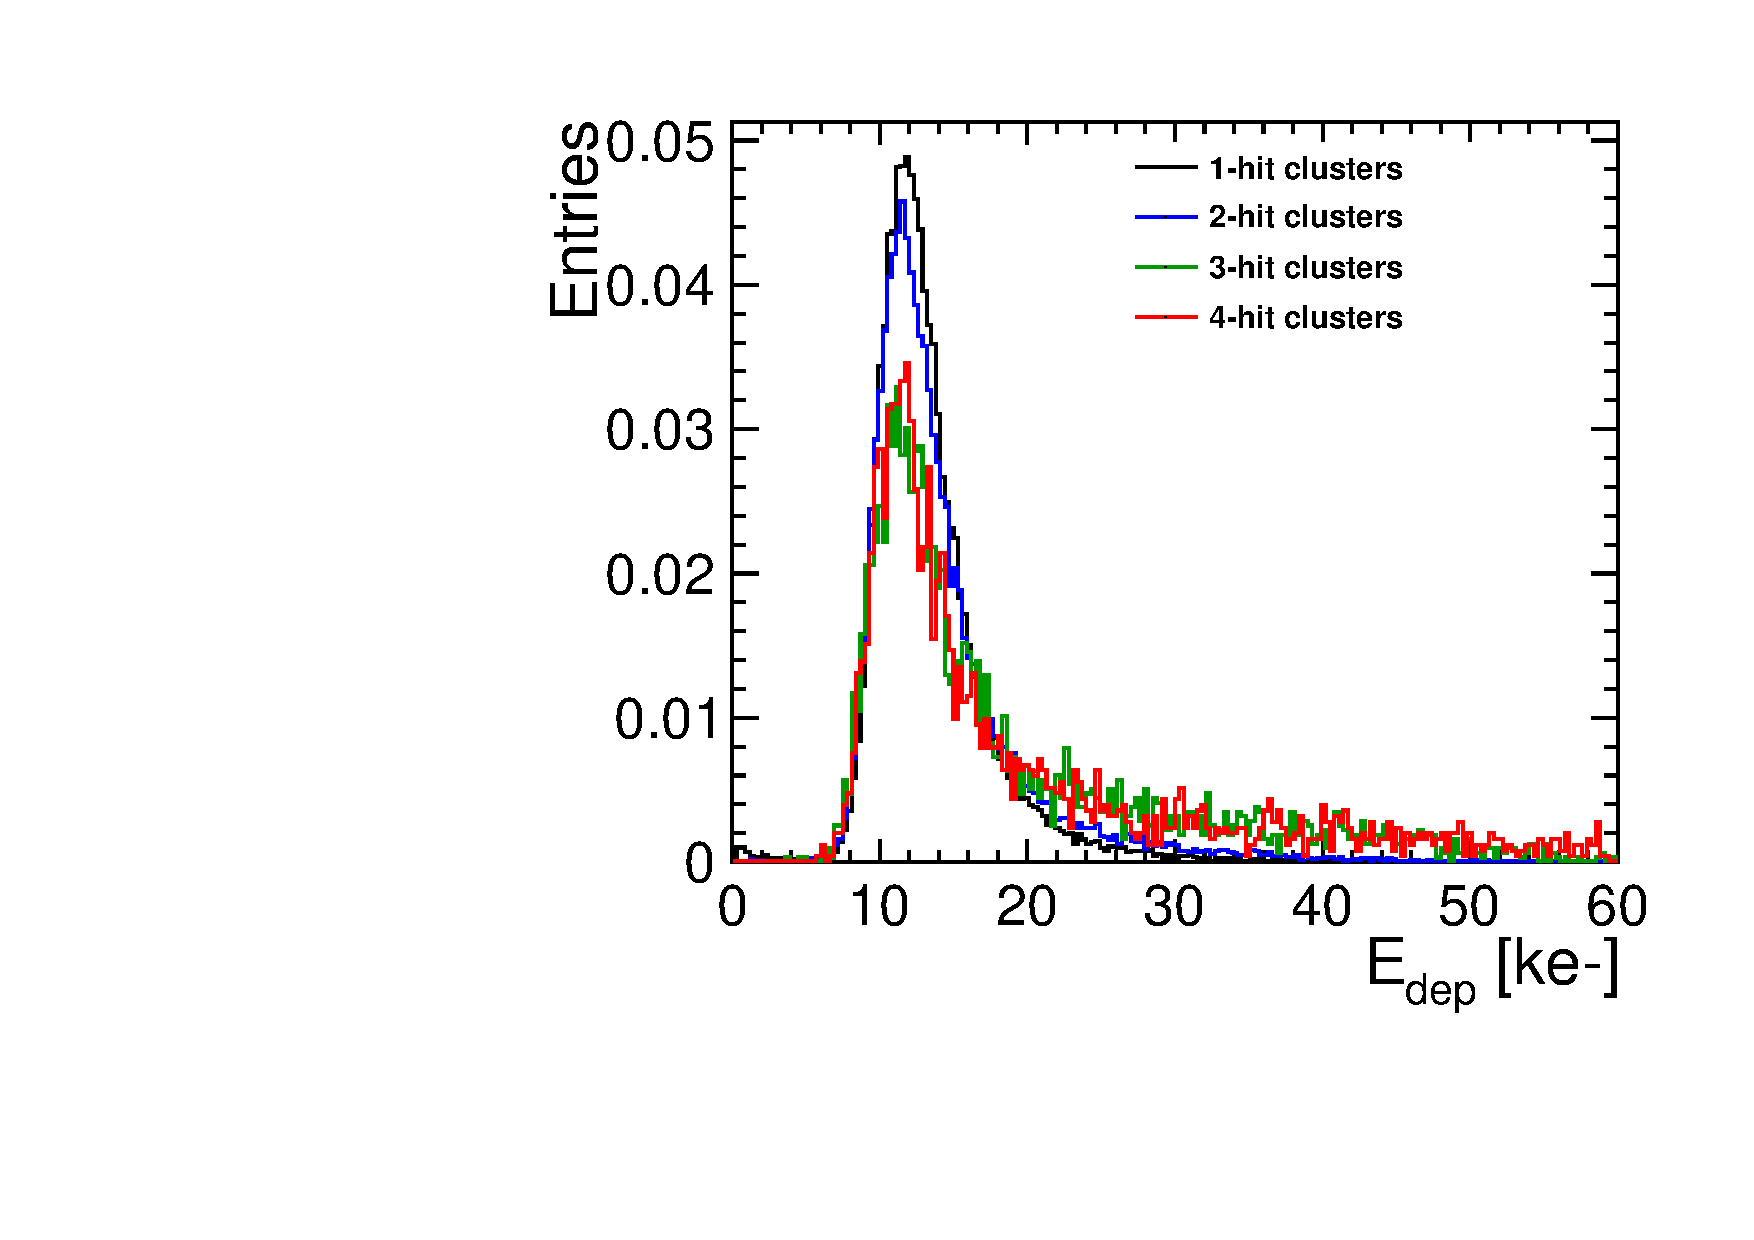
\includegraphics[width=\textwidth]{./figures/Calibration/Edep_Clusters_W0005_F01.pdf}
    \caption{W5\_F1}
  \end{subfigure}
  \caption{Energy deposition distribution for one, two, three and
    four-pixel clusters for assemblies with (a) $50\,\micron$, (b)
    $100\,\micron$ and (c) $150\,\micron$ thick planar sensors.}
  \label{sec:testBeamDataCalibrated_Edep}
\end{figure}

% For all assemblies, the energy deposition in electrons is given in
% \cref{sec:appendixCalibDataG4}.

\cref{fig:G4_simu_data_Edep} compares the total energy deposition in a
cluster in data and simulation for all cluster sizes combined. The
most-probable-value and the width of the distributions in data and
simulation agree. Therefore the calibration is validated using the
test-beam data. For the simulation, the PAI physics list is used which
provides an energy deposition spectrum similar to the Bichsel
distribution (see \cref{fig:BichselVSG4}). This confirms that the
Bichsel model describes well the energy deposition in thin silicon
sensors.

\begin{figure}[htbp] \centering
  \begin{subfigure}[b]{0.3\textwidth}
    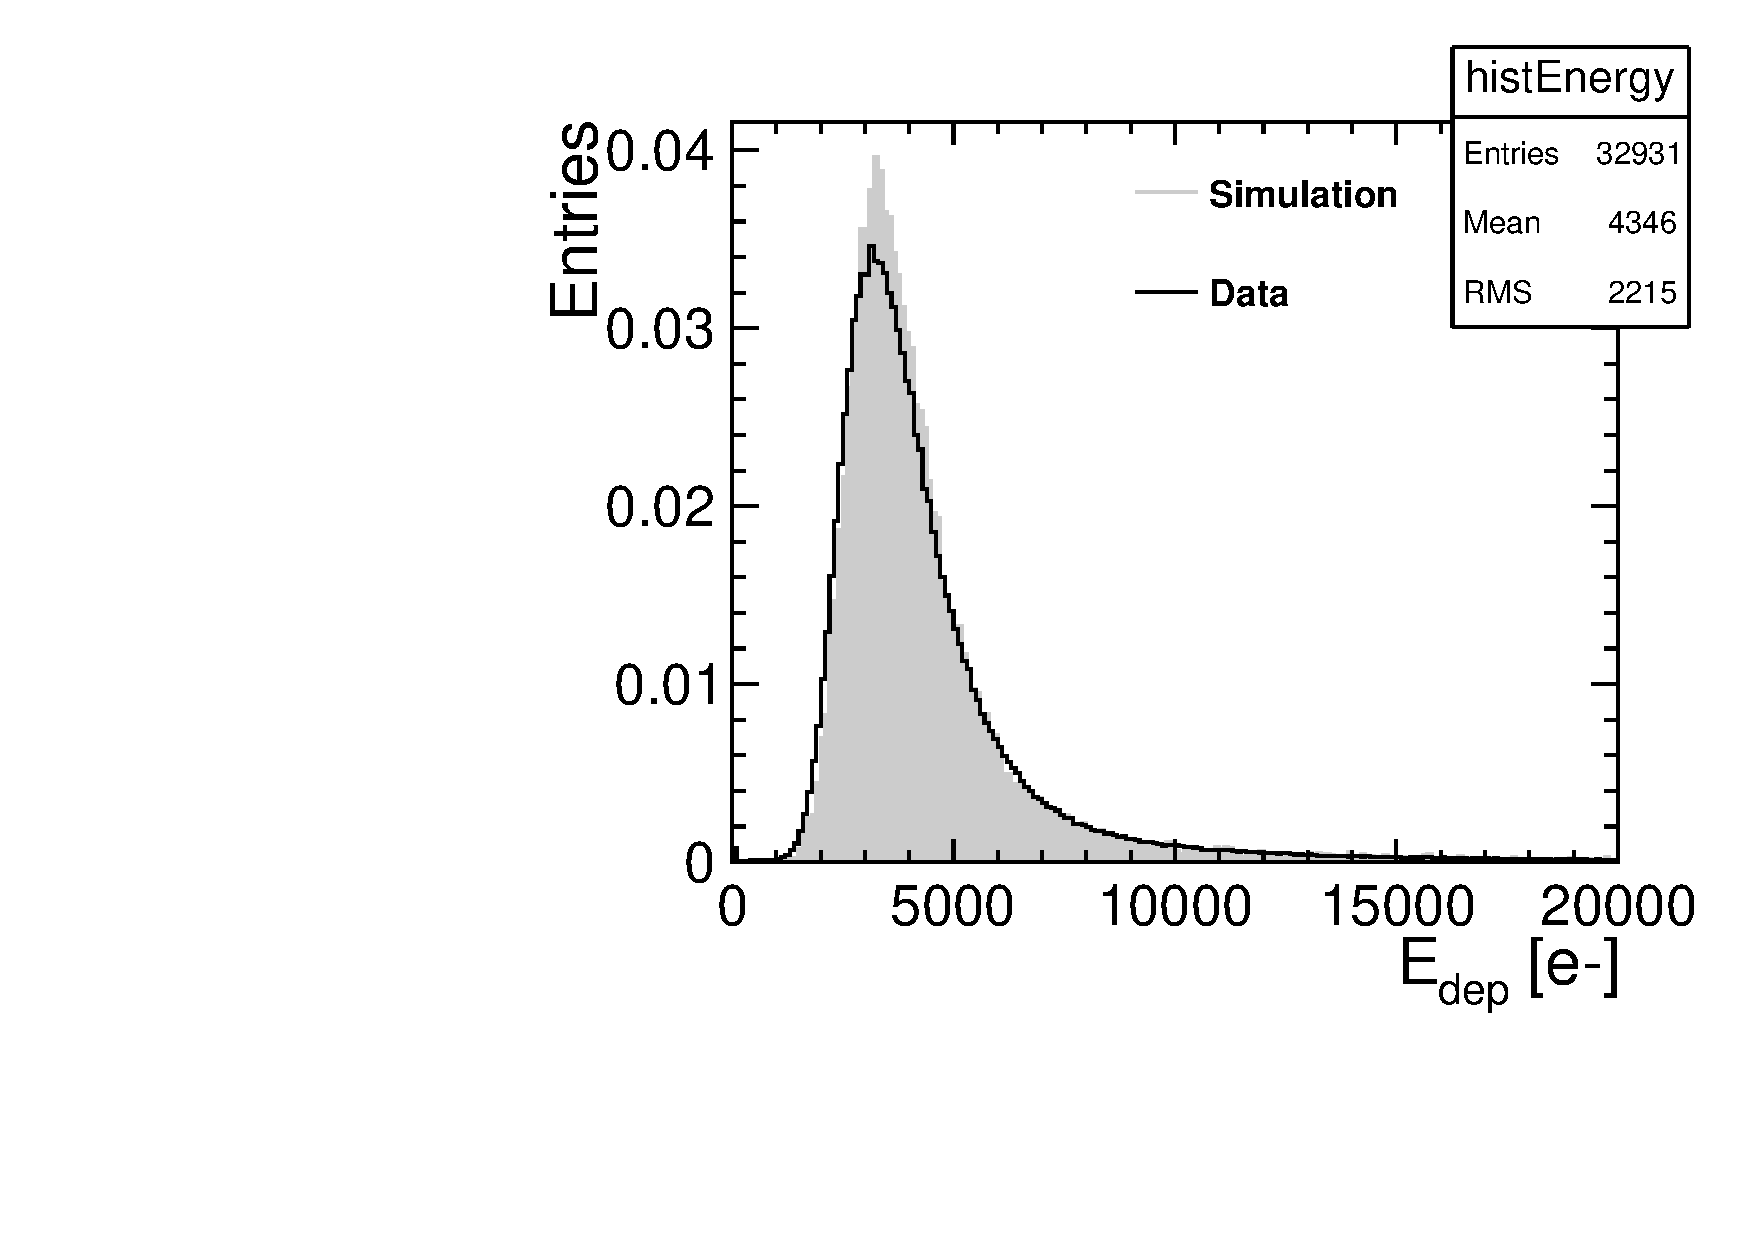
\includegraphics[width=\textwidth]{figures/TestBeam/50micron_Edep.pdf}
    \caption{W19\_G7}
  \end{subfigure} \hfill
  \begin{subfigure}[b]{0.3\textwidth}
    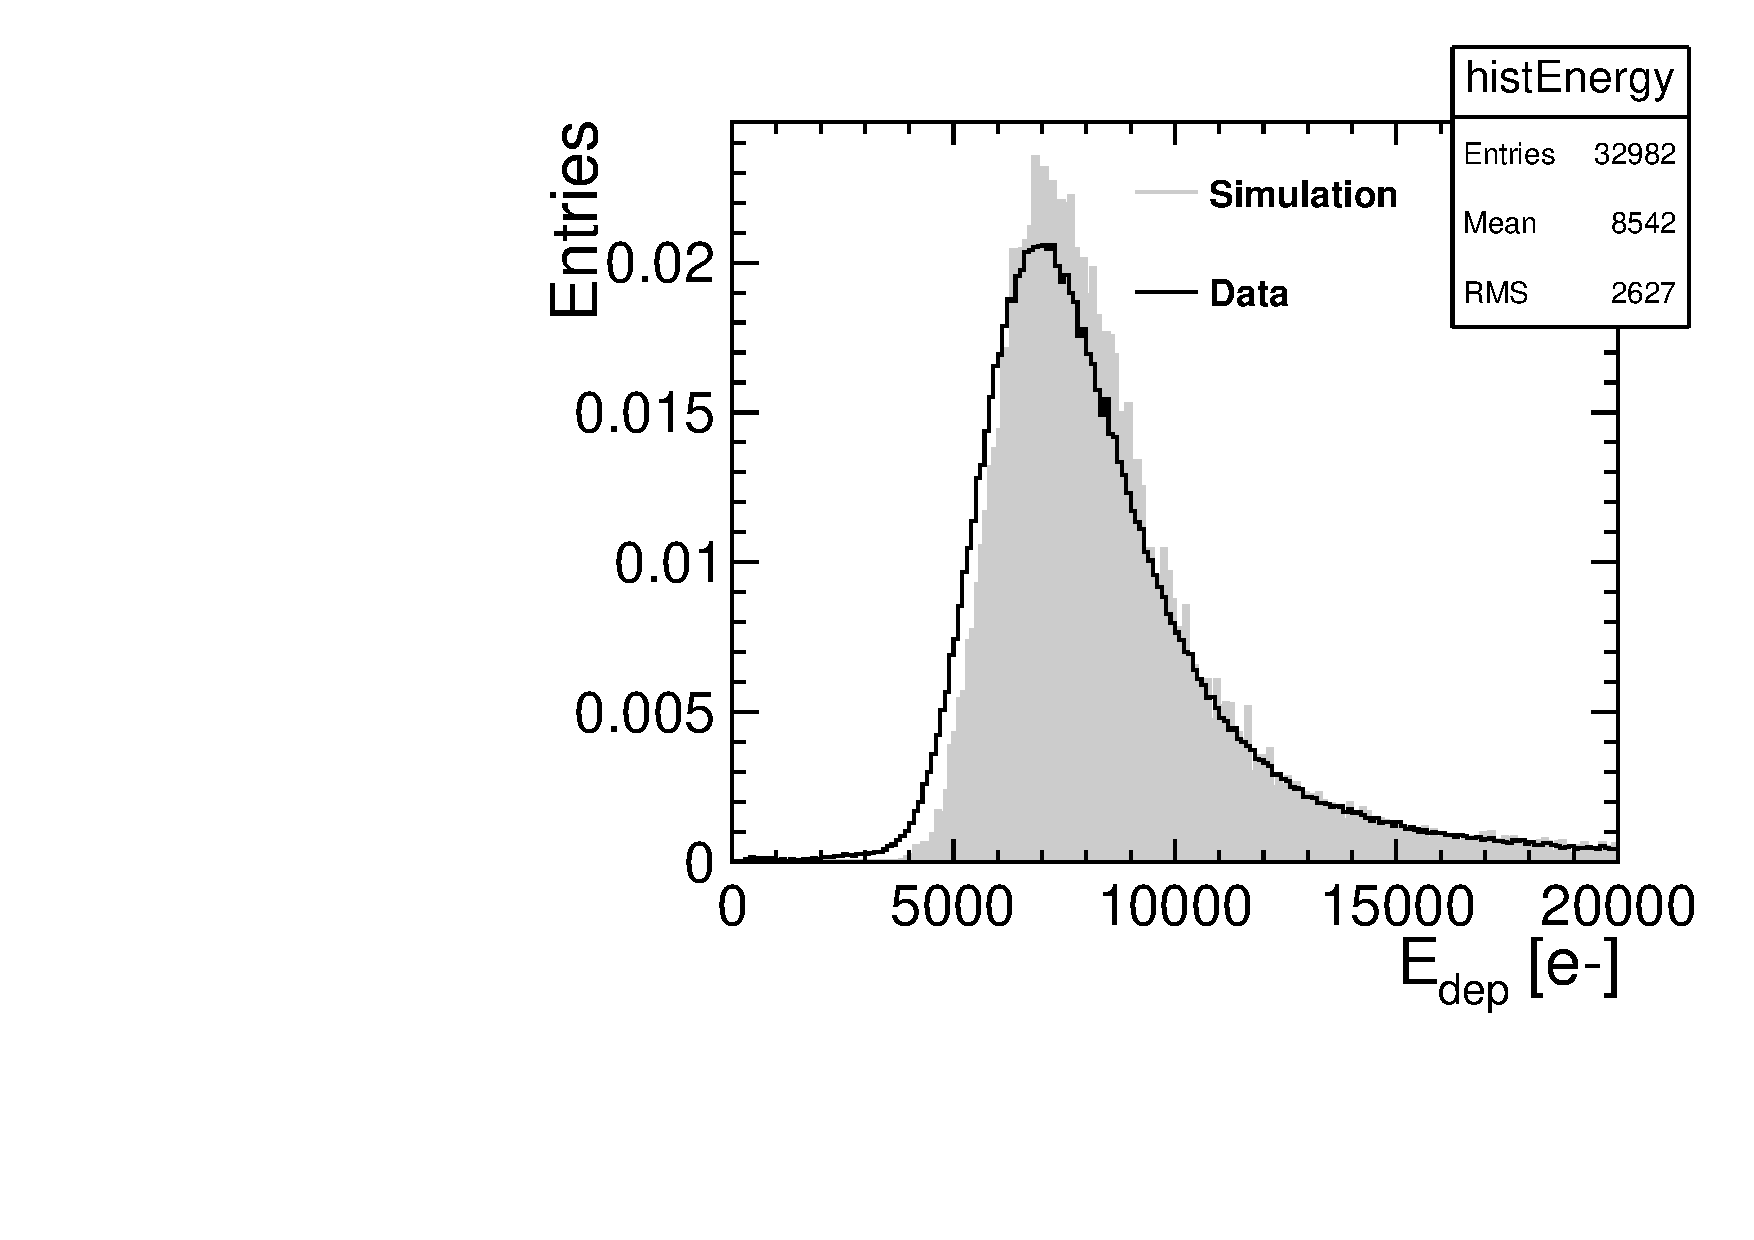
\includegraphics[width=\textwidth]{figures/TestBeam/100micron_Edep.pdf}
    \caption{W5\_E2}
  \end{subfigure} \hfill
  \begin{subfigure}[b]{0.3\textwidth}
    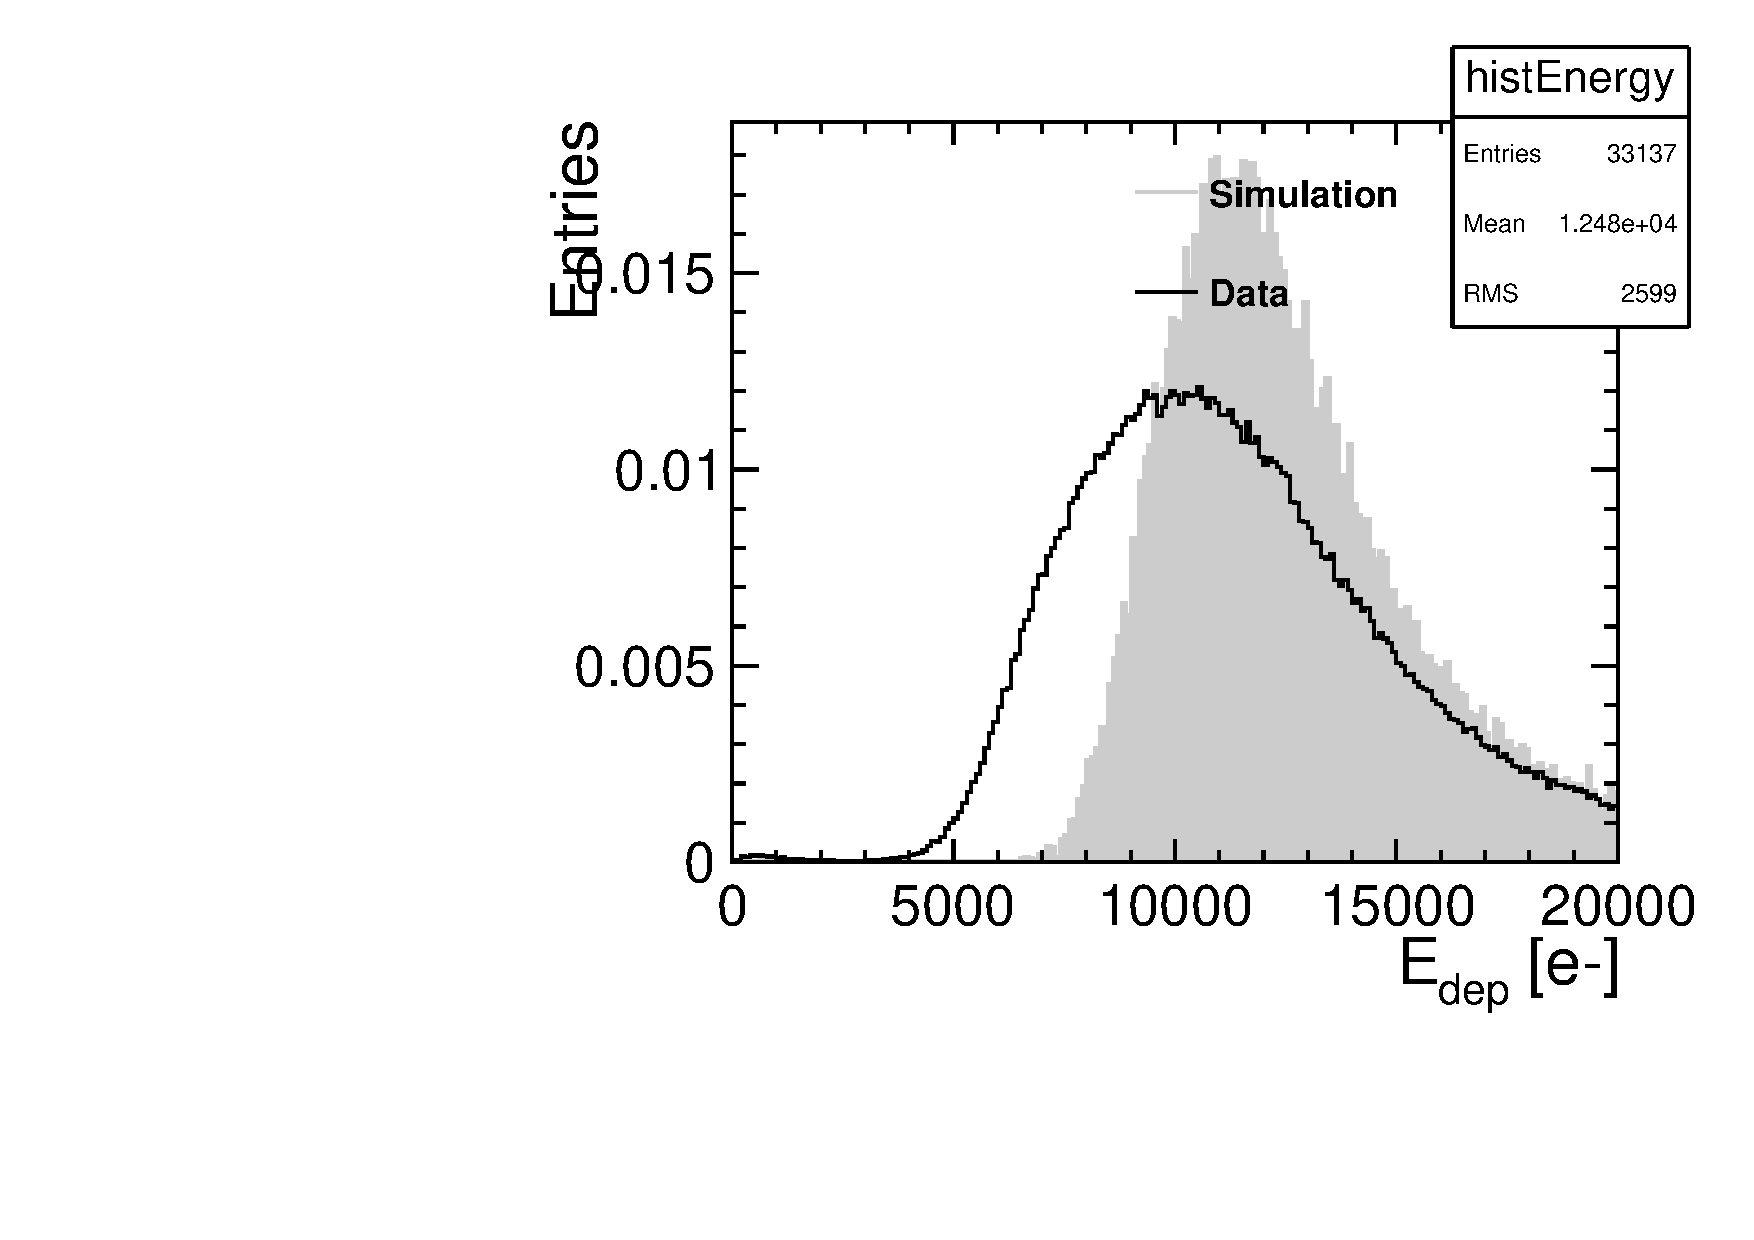
\includegraphics[width=\textwidth]{figures/TestBeam/150micron_Edep.pdf}
    \caption{W5\_F1}
  \end{subfigure} 
  %% \hfill
  %% \begin{subfigure}[b]{0.23\textwidth}

  %%   \caption{$300\,\micron$}
  %% \end{subfigure}
  \caption{The energy deposition for all cluster sizes in simulation
    and data for (a) $50\,\micron$, (b) $100\,\micron$ and (c)
    $150\,\micron$ thick planar sensors. The assemblies are operated
    at nominal conditions.}
  \label{fig:G4_simu_data_Edep}
\end{figure}



%% --------------------------------------------- %%
\subsection{Measurement of the depletion voltage}
\label{sec:ThinSensors_depletionVoltage}

The depletion voltage corresponds to the voltage at which the sensor
is fully depleted and the charge is collected over the full thickness
of the sensor. In normal operation, only the charge created in the
depletion region can be detected. The sensor should be fully depleted
to collect the maximal signal charge possible. The depletion voltage
can be measured in test beams by scanning the bias voltage. The
depletion voltage and the sensor thickness are related by
\cref{eq:depletionVoltage}. For lower bias voltages the sensor is
under depleted, therefore the collected charge is reduced and is
proportional to the square root of the bias voltage. After reaching
the depletion voltage, the collected charge displays a plateau.

To obtain the depletion voltage, first, the distribution of the
deposited energy in the sensor is fitted with a landau function
convoluted with a Gaussian. The fit is done using
RooFit~\cite{Cranmer:2012sba} and an example is given in
\cref{fig:W5_F1_DepletionVoltage_TOTdistr}.
\cref{fig:W2_J5_DepletionVoltage_chargeVSbiasVoltage} shows the
most-probable-value (MPV) of the measured energy deposition as a
function of the square root of the bias voltage. In this figure, two
distinct regions can be seen: a sloped region and a plateau
region. The depletion voltage of the assembly is obtained by
calculating the intersection of a linear fit performed on both regions
(defined by eye). The calculated depletion voltages for all assemblies
are summarised in \cref{tab:depletionVoltage,fig:depletionVoltage}.

% The $50\,\micron$ thick sensor is depleted at a low bias voltage of
% $\sim$2~V. However the measurement was done with a voltage step size
% of $1$~V and the fits give a higher depletion voltage of $\sim7$~V.

From the depletion voltage, the concentration of the dopants in the
bulk is calculated to be around
$N_{bulk}\approx1.3\,\inversemetercubic$ and corresponds to a
resistivity of $\rho\approx10\,\text{k}\Omega\,\text{cm}$ for all
assemblies. The assemblies are confirmed to have high-resistivity
silicon sensors. They are optimal for tracking detectors since it is
possible to fully deplete them and high electric fields provide fast
and efficient charge collection. The depletion voltage and the doping
concentration are used as input for the simulation of these
assemblies.

\begin{figure}[htbp]\centering
  \begin{subfigure}[b]{0.45\textwidth}
  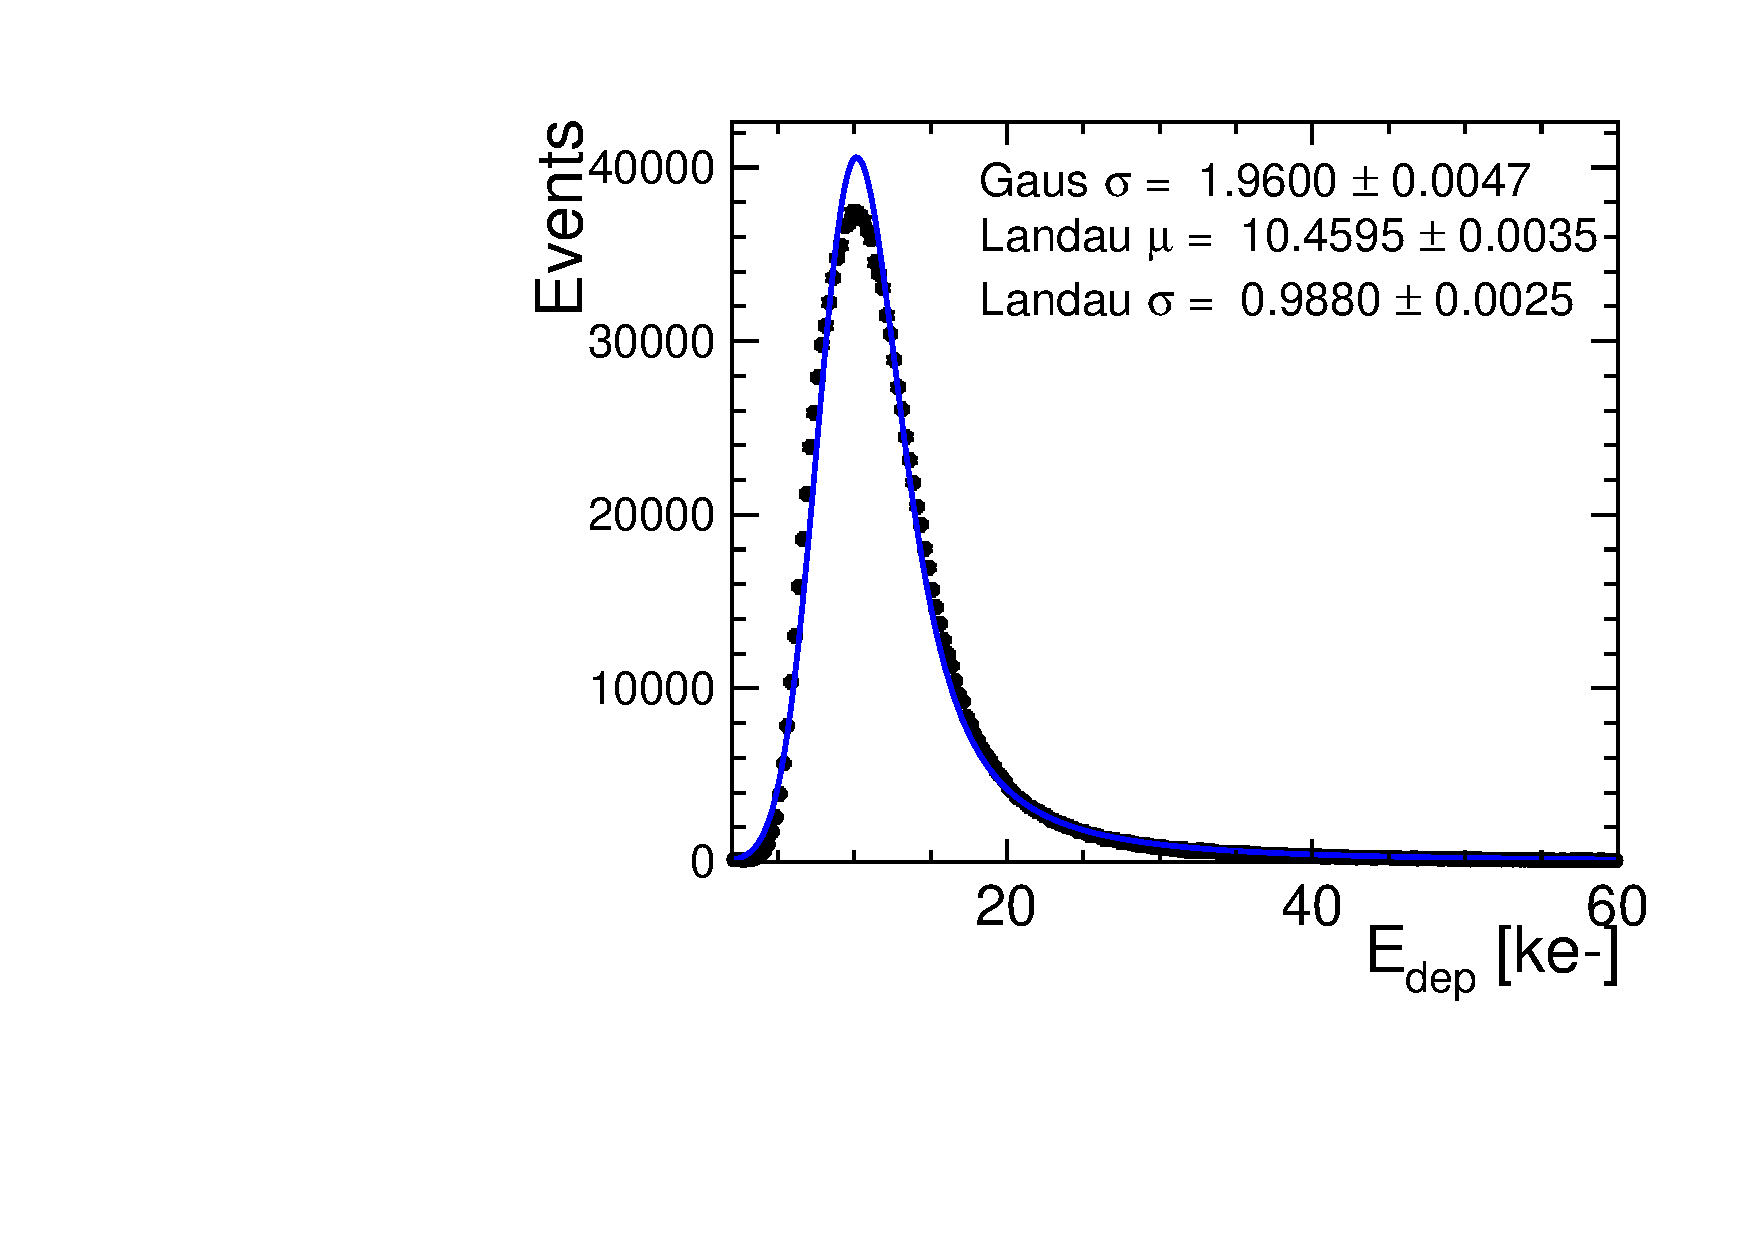
\includegraphics[width=\textwidth]{./figures/TestBeam/W5_F1_totalTOT_Langau_run761.pdf}
  % W2_J5_totalTOT_Langau_run1998.pdf}
  \caption{}\label{fig:W5_F1_DepletionVoltage_TOTdistr}
  \end{subfigure} \hfill
  \begin{subfigure}[b]{0.45\textwidth}
    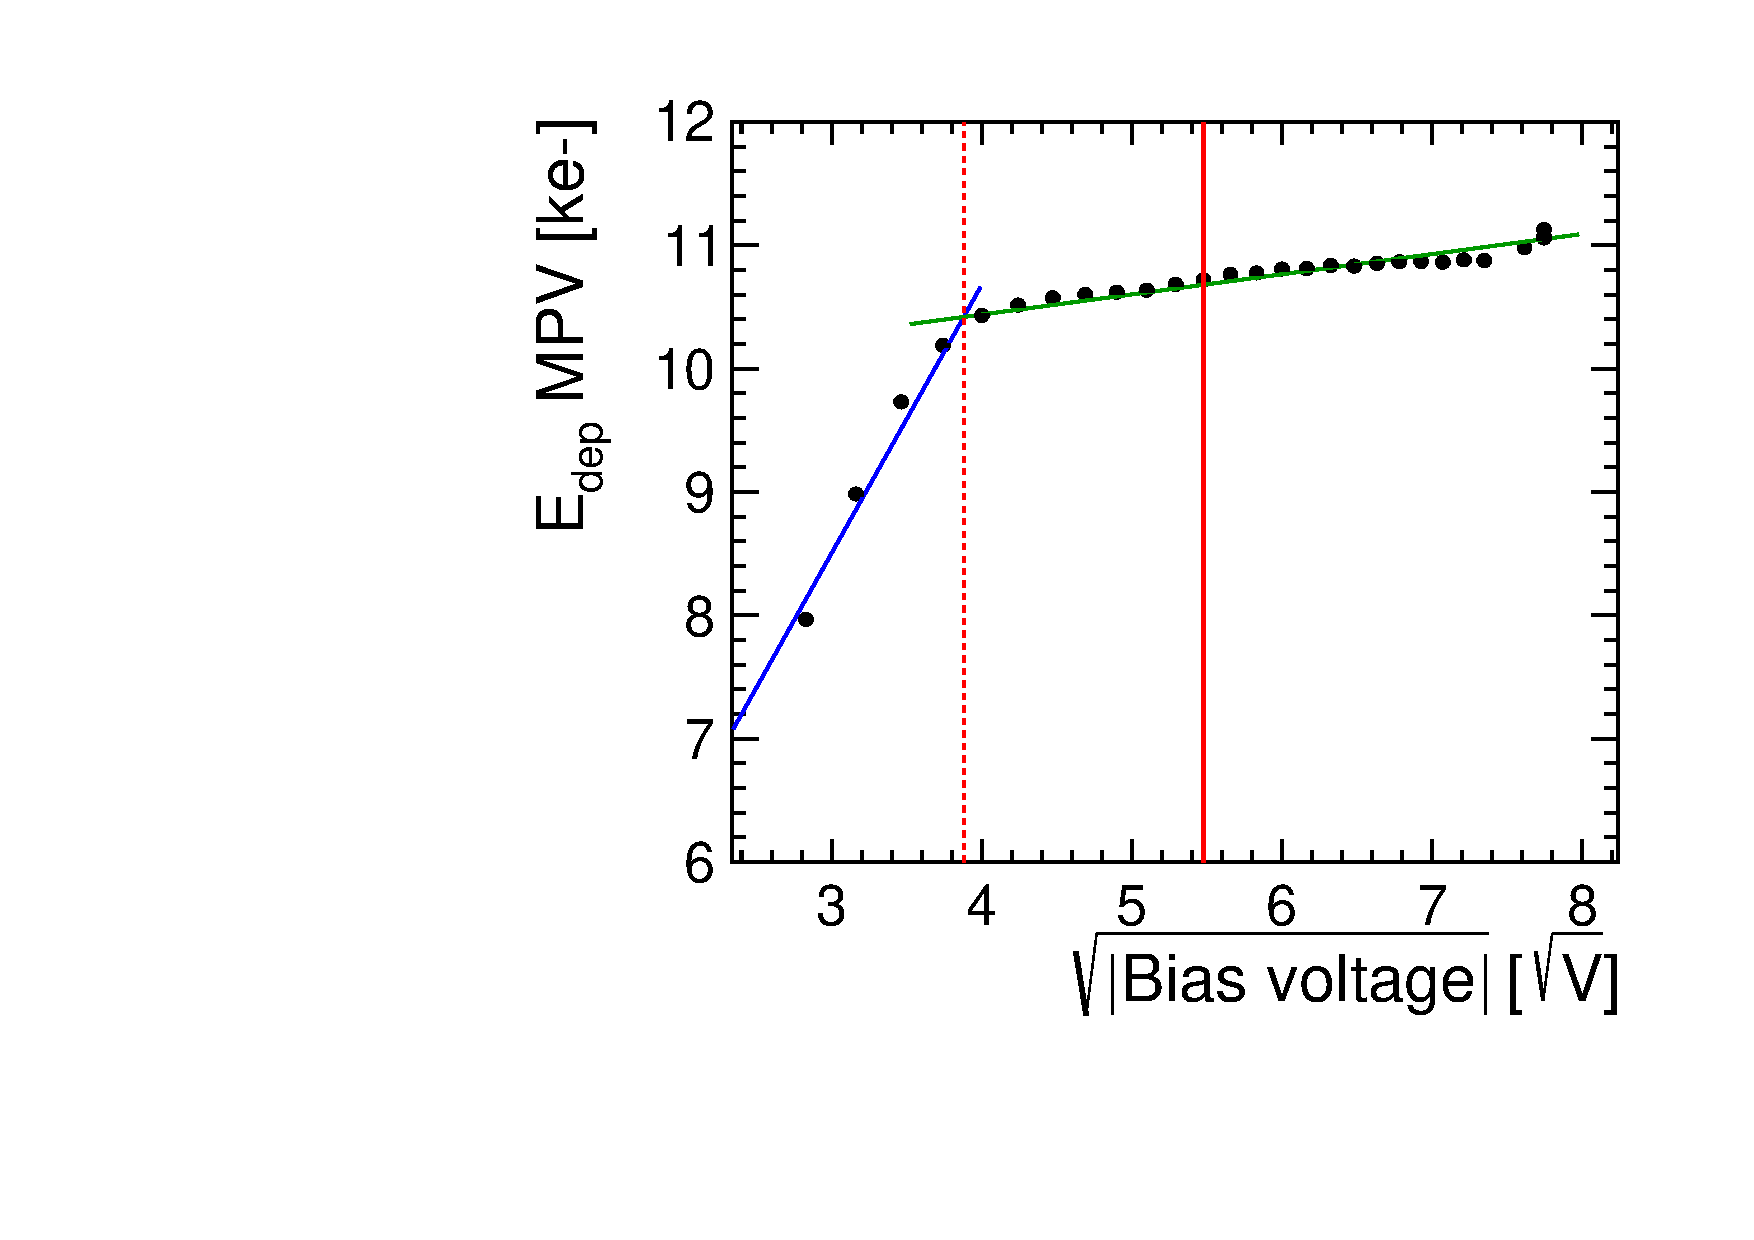
\includegraphics[width=\textwidth]{./figures/TestBeam/depletionVoltage_W0005_F01_Edep.pdf}
    \caption{}\label{fig:W2_J5_DepletionVoltage_chargeVSbiasVoltage}
  \end{subfigure}
  \caption{(a) The measured energy deposition distribution in a
    $150\,\micron$ thick silicon sensor (W5\_F1) with a bias voltage
    of -30~V fitted with a Landau function convoluted with a Gaussian
    function. (b) The most probable value of the measured energy
    deposition as a function of the bias voltage for W5\_F1. Straight
    lines are used to fit the slope and the plateau regions. The
    depletion voltage corresponds to the intersection of these two
    regions and shown in a red dashed line. The continuous red line
    shows the nominal operating bias voltage.}
  \label{fig:W5_F1_DepletionVoltage}
\end{figure}

\begin{table}[htbp]
  \centering
  \caption{Measured depletion voltage for the assemblies described in
    \cref{tab:Timepix3Assemblies} and calculated by fitting the
    plateau and slope regions of TOT as a function of the bias
    voltage.}
  \label{tab:depletionVoltage}
  \begin{tabular}{lc}
    \toprule
    Assembly & Depletion voltage [V] \\
    \midrule
    W19\_G7 & -7 \\
    W19\_F7 & -7\\
    W19\_L8 & -7\\
    W19\_C7 & -7\\ \hline
    W5\_E2 & -12 \\ \hline
    W5\_F1 & -15 \\ %\hline
%    W2\_J5 & 63.23 \\ 
    \bottomrule
  \end{tabular}
\end{table}

%% --------------------------------------------- %%
\subsection{Cluster size distribution}
The cluster size distribution is an indication for the amount of
charge sharing in a sensor. For thicker sensors, more charge sharing
is expected since the charge drifts over a longer distance and
diffuses across a larger transverse area. The threshold of the readout
electronics has a large impact on the detection of the charge
sharing. The threshold should be as low as possible to avoid
undetected energy deposits.

In this analysis, the hit pixels form a cluster with a distance
criterion of $\sqrt{2}\times$pitch\footnote{The distance between the
  center of pixels sharing the same edges is $1\times$pitch and for
  pixels sharing common corners is $\sqrt{2}\times$pitch.}: pixels
sharing common corners or edges are considered as clusters. For sensor
thicknesses in the range of $50\,\micron$-$150\,\micron$, clusters of
size one to four are expected due to diffusion. Larger clusters are
expected due to other effects such as $\delta$-rays. The most common
cluster shapes are illustrated in \cref{tab:clusizeShapes}.

\begin{table}
  \centering
  \caption{Most common cluster shapes.}
  \label{tab:clusizeShapes}
  \begin{tabular}{ccccc}
    \toprule
    Shape & Cluster size & Size in $x$ & Size in $y$ & Name \\
    \midrule
    \begin{tikzpicture}
      \draw (0,0) rectangle (0.5,-0.5);
    \end{tikzpicture}
    & 1 & 1 & 1 & size 1 ($1\times1$) \\
    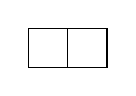
\begin{tikzpicture}
      \draw (0.0,0.0) rectangle (0.5,-0.5);
      \draw (0.5,0.0) rectangle (1.0,-0.5);
    \end{tikzpicture}
    & 2 & 2 & 1 & size 2 ($2\times1$) \\
    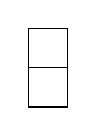
\begin{tikzpicture}
      \draw (0.0,0.0) rectangle (0.5,-0.5);
      \draw (0.0,0.5) rectangle (0.5,0.0);
    \end{tikzpicture}
    & 2 & 1 & 2 & size 2 ($1\times2$) \\
    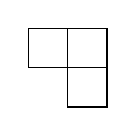
\begin{tikzpicture}
      \draw (0.0,0.0) rectangle (0.5,-0.5);
      \draw (0.5,-0.5) rectangle (1.0,-1.0);
      \draw (0.5,0.0) rectangle (1.0,-0.5);
    \end{tikzpicture}
    & 3 & 2 & 2 & size 3 ($2\times2$)\\
    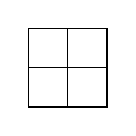
\begin{tikzpicture}
      \draw (0.0,0.0) rectangle (0.5,-0.5);
      \draw (0.5,-0.5) rectangle (1.0,-1.0);
      \draw (0.5,0.0) rectangle (1.0,-0.5);
      \draw (0.0,-0.5) rectangle (0.5,-1.0);
    \end{tikzpicture}
    & 4 & 2 & 2 & size 4 ($2\times2$) \\
    \bottomrule
  \end{tabular}
\end{table}

\cref{fig:G4_simu_data_cluSize} compares the cluster-size distribution
in simulations and data for the assemblies operated at nominal
conditions. There is a good agreement between simulation and data
within $2\%$.

\begin{figure}[htbp] \centering
  \begin{subfigure}[b]{0.3\textwidth}
    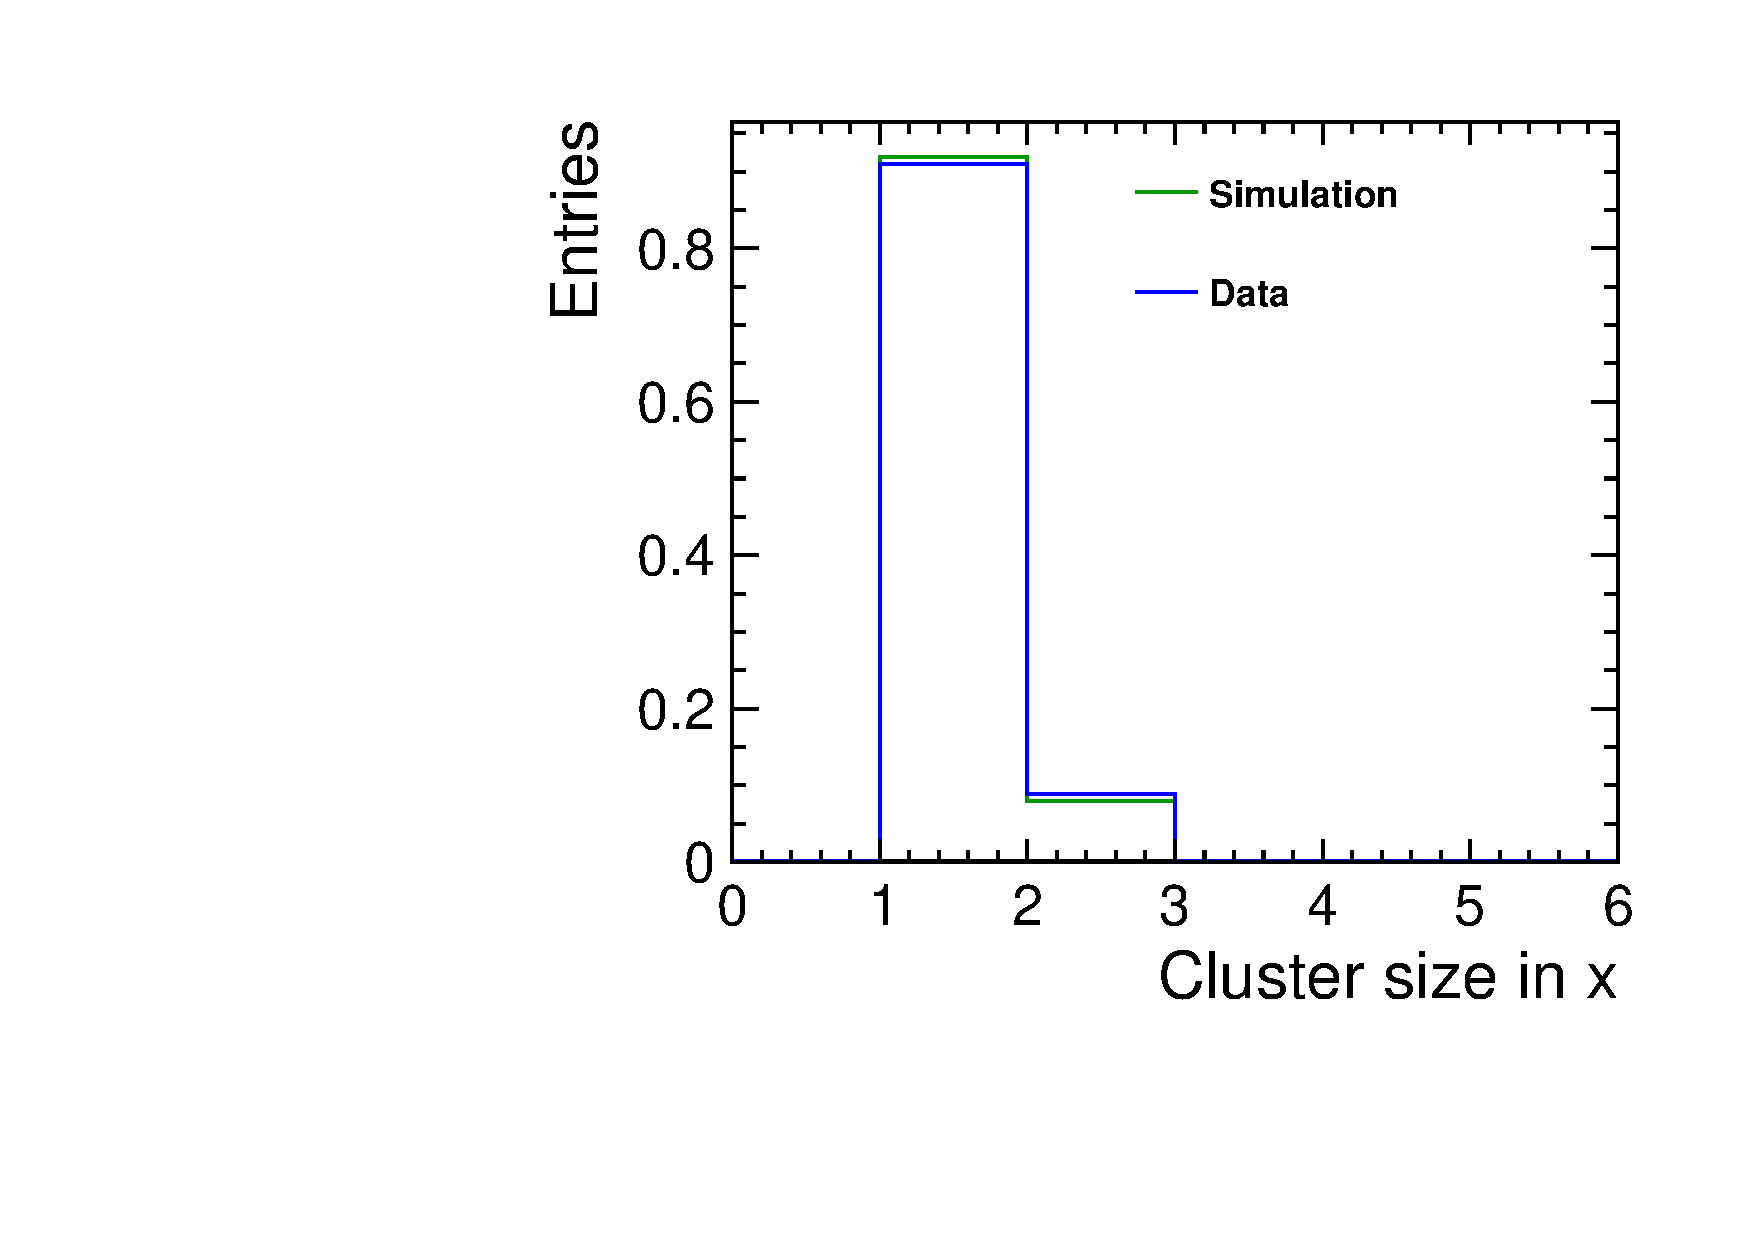
\includegraphics[width=\textwidth]{figures/TestBeam/50micron_sizeX.pdf}
    \caption{$50\,\micron$ (W19\_G7)}
  \end{subfigure} \hfill
  \begin{subfigure}[b]{0.3\textwidth}
    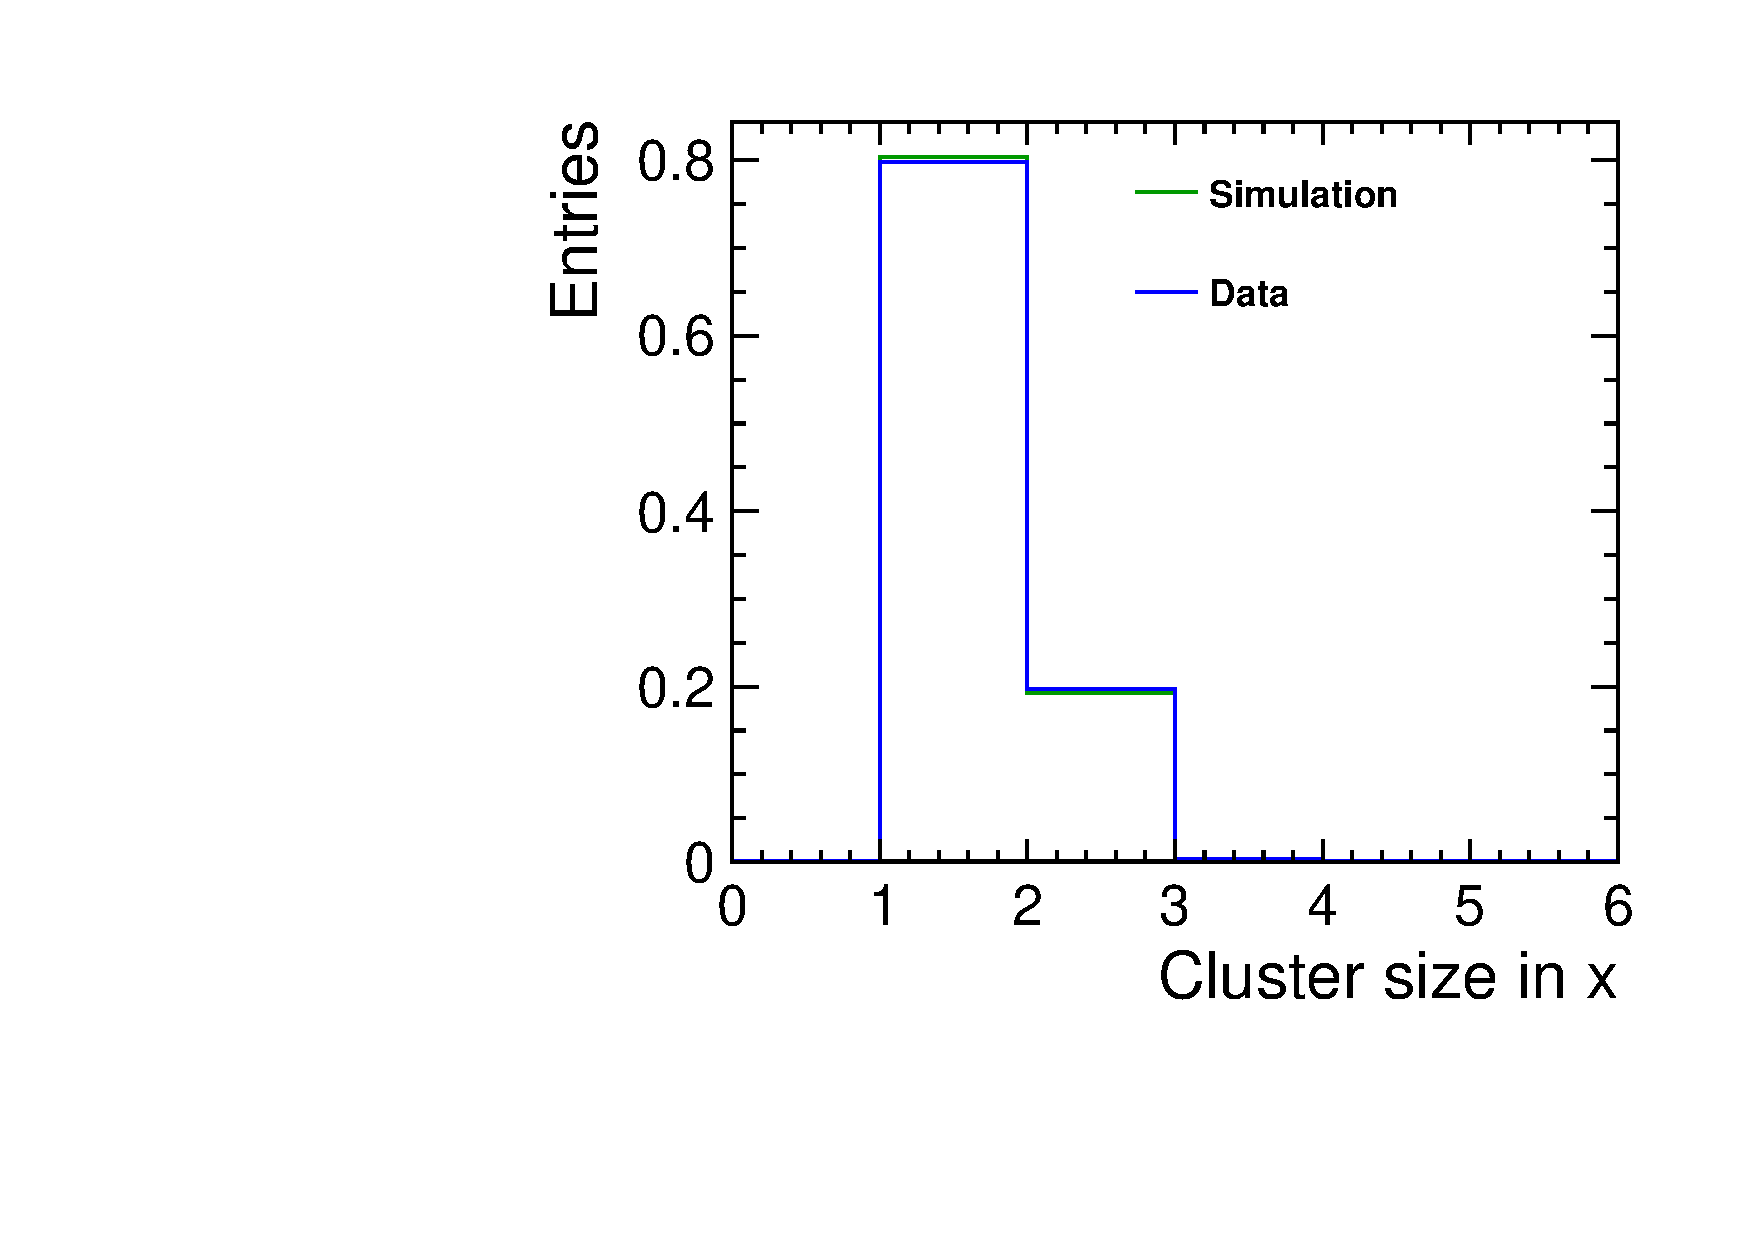
\includegraphics[width=\textwidth]{figures/TestBeam/100micron_sizeX.pdf}
    \caption{$100\,\micron$ (W5\_E2)}
  \end{subfigure} \hfill
  \begin{subfigure}[b]{0.3\textwidth}
    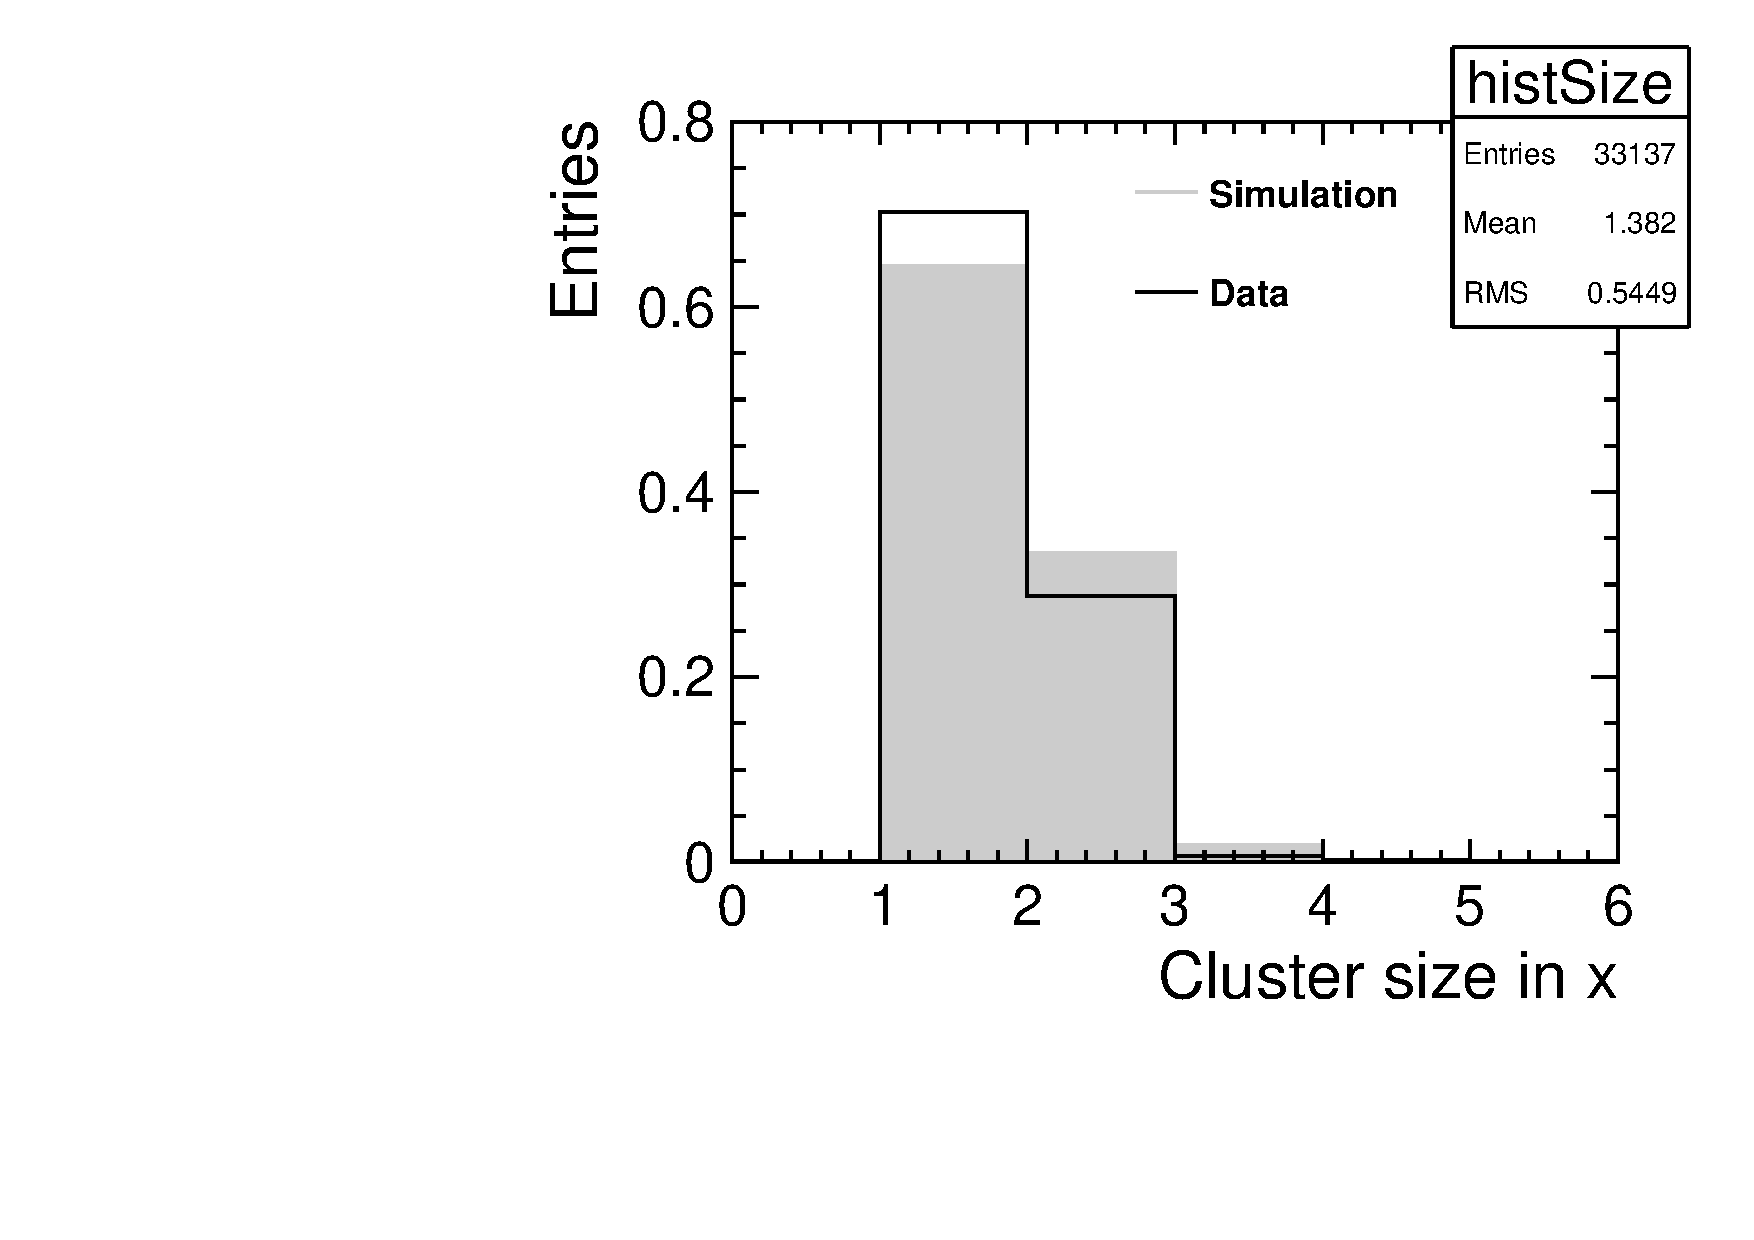
\includegraphics[width=\textwidth]{figures/TestBeam/150micron_sizeX.pdf}
    \caption{$150\,\micron$ (W5\_F1)}
  \end{subfigure} 
  %% \hfill
  %% \begin{subfigure}[b]{0.23\textwidth}

  %%   \caption{$300\,\micron$ p-in-n}
  %% \end{subfigure}
  \caption{The cluster size distribution in simulation and data for
    $50\,\micron$, $100\,\micron$ and $150\,\micron$ thick
    sensors. The assemblies are operated at nominal conditions.}
  \label{fig:G4_simu_data_cluSize}
\end{figure}


The fraction of different cluster sizes depends on the operating
conditions of the assemblies like the bias voltage and the threshold
of the readout ASICs. \cref{fig:cluSize_operatingConditions} shows the
cluster size fraction for a $150\,\micron$ thick sensor (assembly
W5\_F1) operated at different bias voltages and thresholds.  

Higher bias voltages reduce the amount of charge sharing since the
drift time is lowered in a stronger electric field and the charges
diffuse less in the transverse direction. For very low bias voltages,
the sensor is under-depleted. An increase in bias voltage in this
regime increases the charge sharing. The pixel neighbouring a hit
pixel is more likely to be over threshold as more charge is
collected. The results for other assemblies are shown in
\cref{fig:clusterSize_vs_biasVoltage}.

Lowering the threshold leads to an increase in the average cluster
size fraction distribution. Results for all assemblies are shown in
\cref{fig:clusterSize_vs_THLscan}.


\begin{figure}[htbp] \centering
  \begin{subfigure}[b]{0.45\textwidth}
    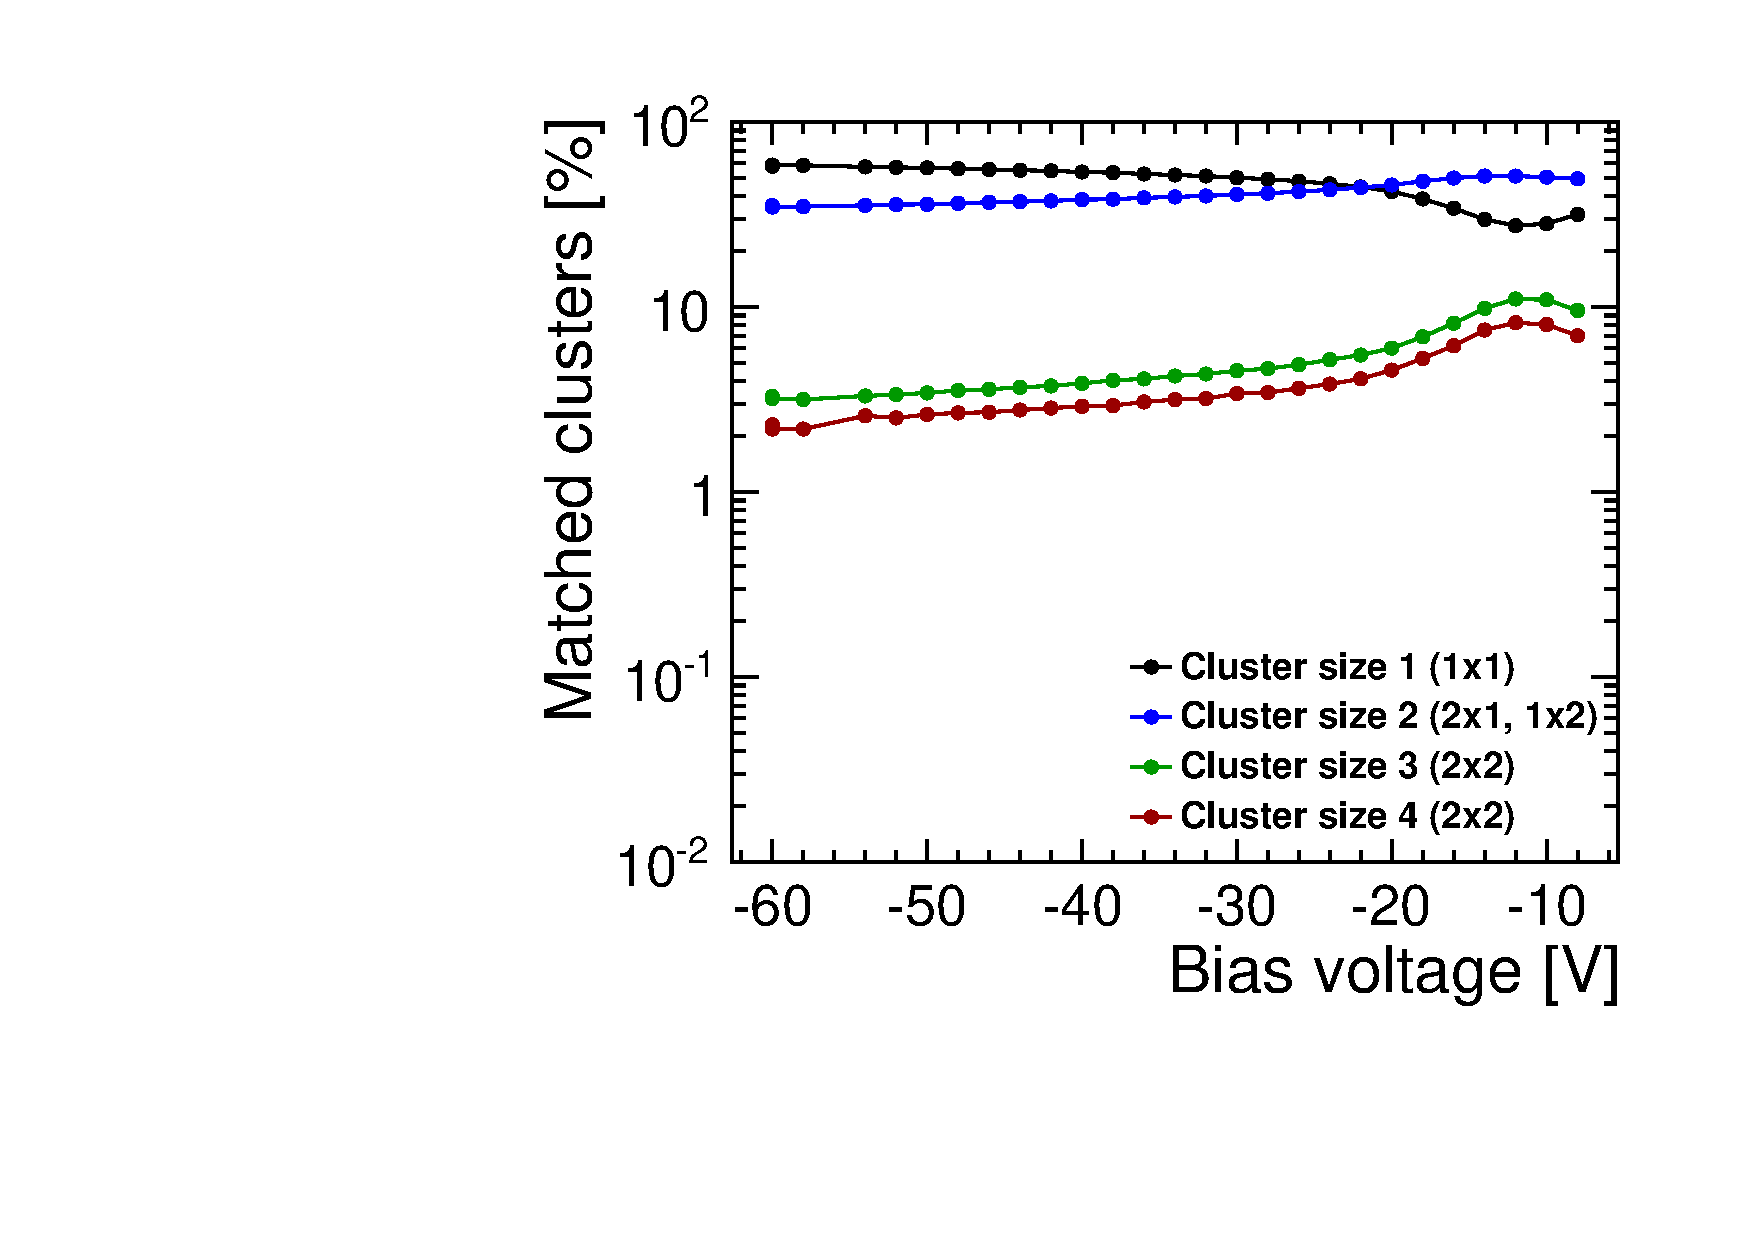
\includegraphics[width=\textwidth]{./figures/TestBeam/cluSize_biasScan_W0005_F01.pdf}
    \caption{}
  \end{subfigure} \hfill
  \begin{subfigure}[b]{0.45\textwidth}
    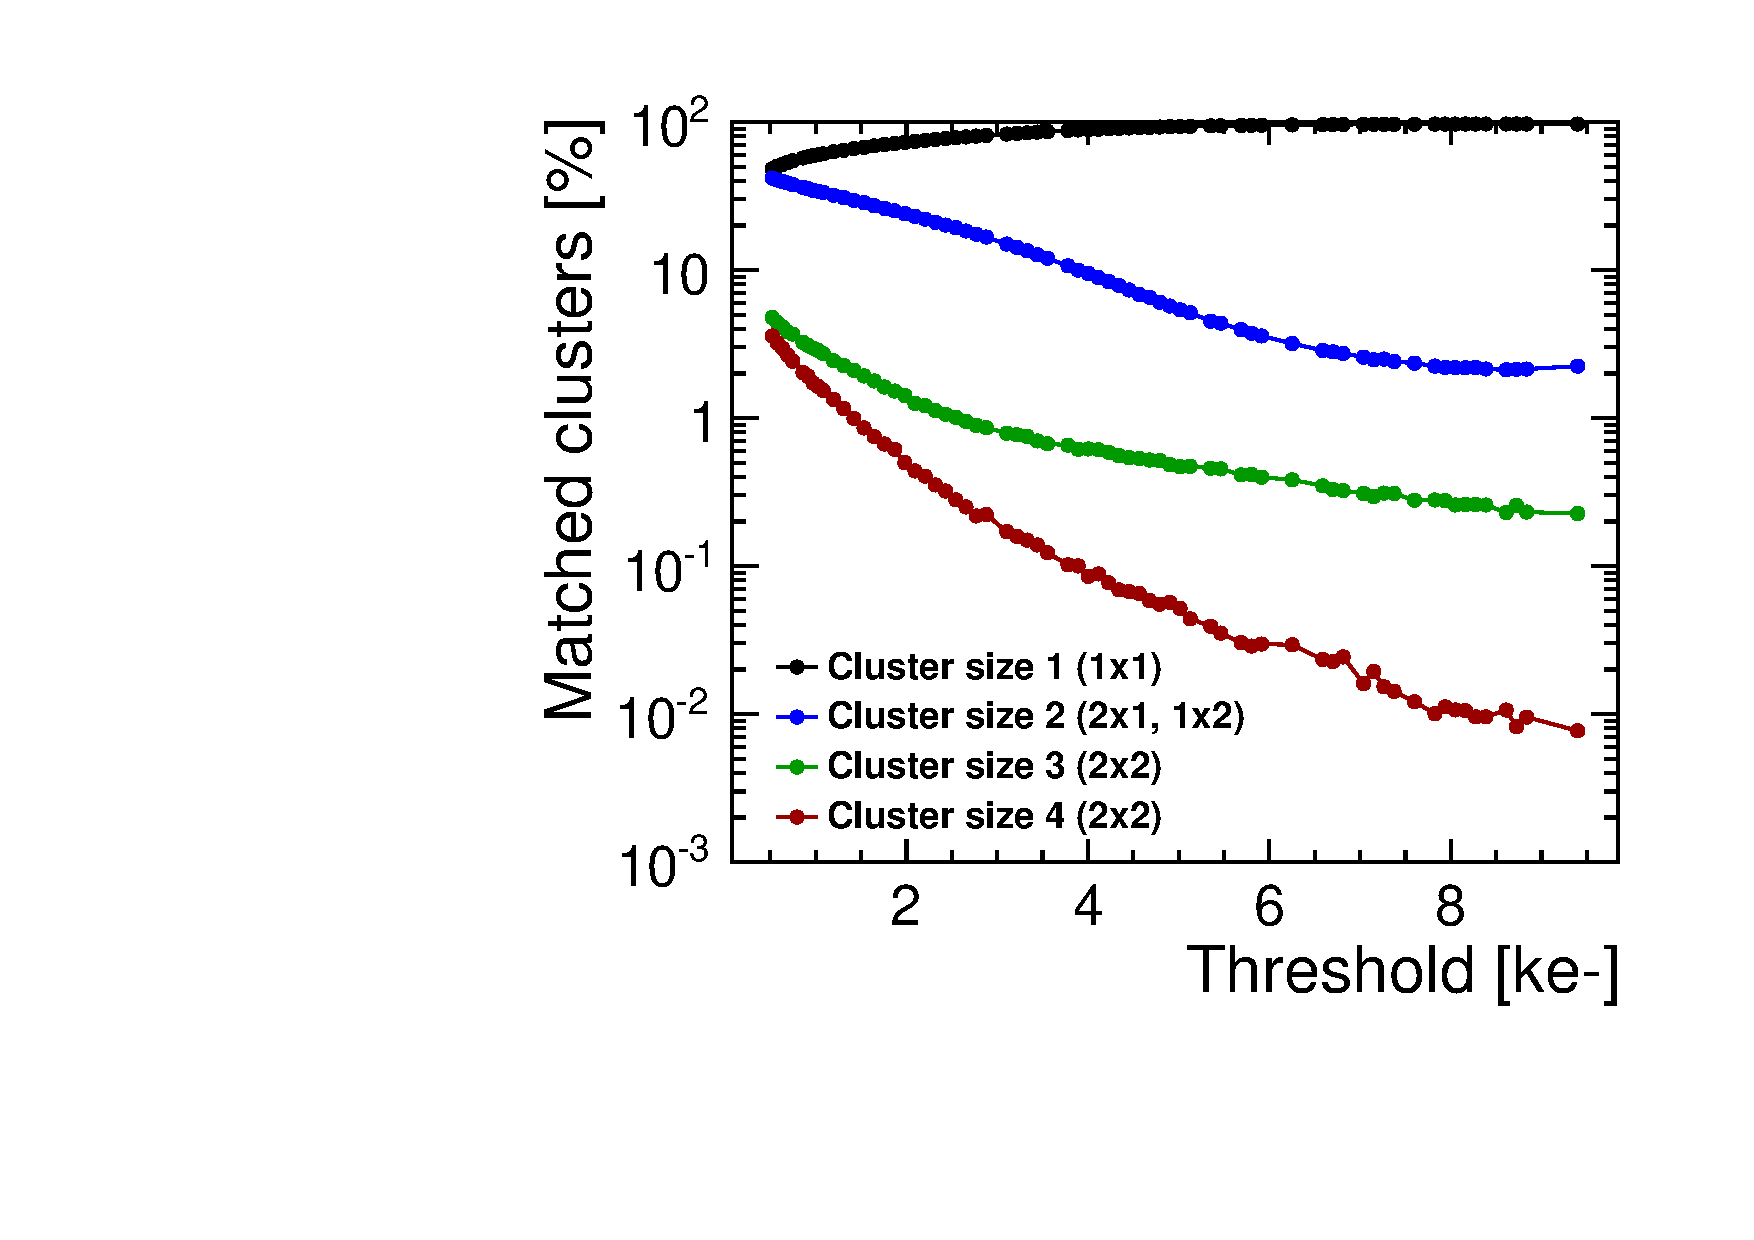
\includegraphics[width=\textwidth]{./figures/TestBeam/cluSize_THLscan_W0005_F01.pdf}
    \caption{}
  \end{subfigure}
  \caption{Cluster-size distribution as a function of (a) bias voltage
    and (b) threshold for the assembly W5\_F1 with a $150\,\micron$
    thick sensor.}
  \label{fig:cluSize_operatingConditions}
\end{figure}


The cluster size fraction as a function of the sensor thickness for
data recorded at the nominal operating conditions is shown in
\cref{fig:cluSize_thickness}. Charge sharing increases with sensor
thickness. The fraction of $1\times2$ and $2\times1$-pixel clusters
are very similar for square pixels and the curve labeled 2-pixel
clusters combine these two cluster geometries. The simulation is in
good agreement with data. Reasonable agreement is observed for high
cluster sizes at $50\,\micron$ sensors which can be explained by the
non-linearity of the calibration curve for low energy deposition and
close to the detection threshold resulting in high uncertainties in
the detected charge measurements. The good agreement between data and
simulation validates the digitiser as described in
\cref{sec:allpix_digitisation}.

\begin{figure}[htbp] 
  \centering
  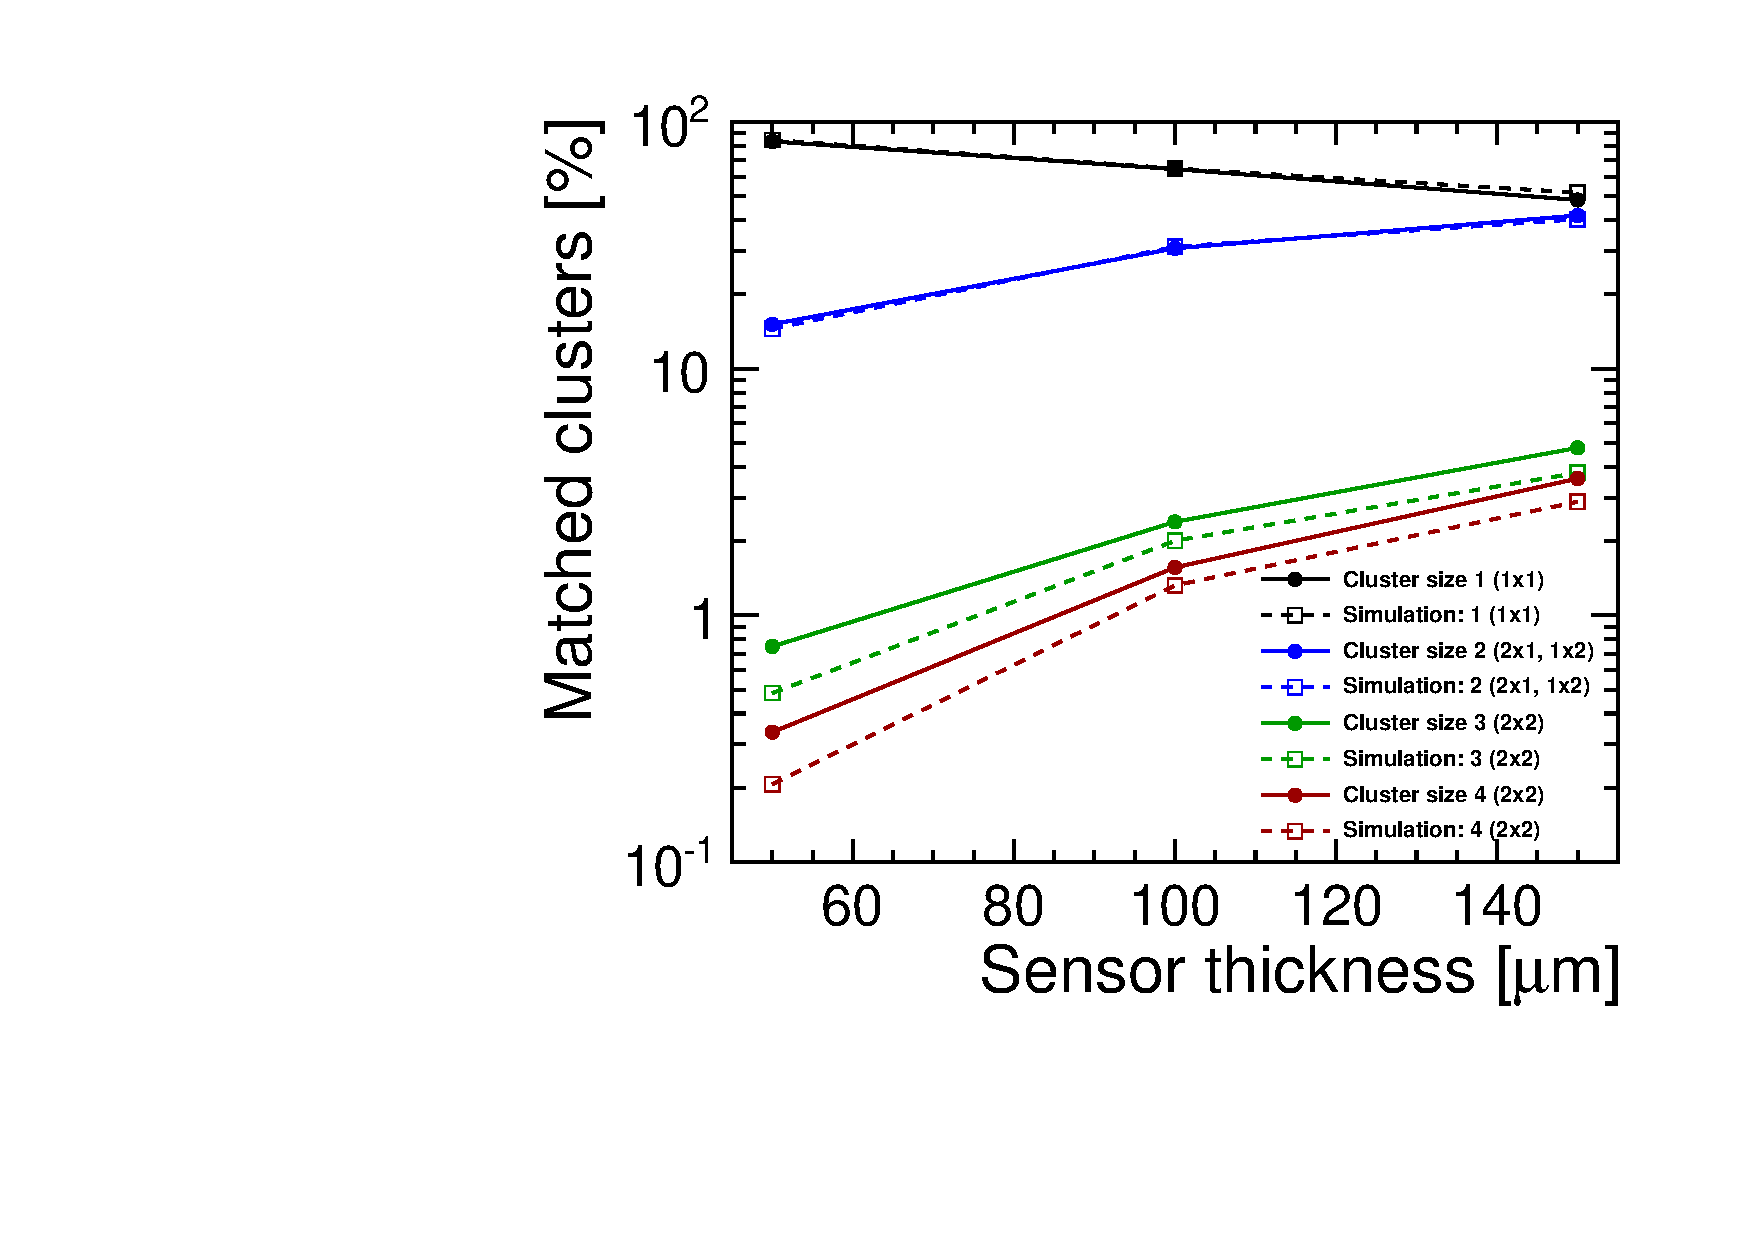
\includegraphics[width=0.5\textwidth]{./figures/TestBeam/cluSize_vs_thickness.pdf}
  \caption{Cluster-size distribution for data and AllPix simulation as
    a function of sensor thickness for runs recorded under nominal
    operating conditions.}
  \label{fig:cluSize_thickness}
\end{figure}

%% --------------------------------------------- %%
\subsection{Charge sharing as a function of the track position}

The charge sharing is studied by extrapolating the track position
obtained from the Timepix3 telescope to the DUT. The size of the
clusters depends on the track position within the pixel. For
perpendicular tracks, multi-pixel clusters are created when the track
hits the edges or the corners of a pixel, leading to sharing of the
charge between the pixel and its neighbouring pixels. The charge
sharing is also affected by the operating threshold of the readout
ASIC. \cref{fig:chargeSharingTrack} illustrates the track position
within the pixel for 1 to 4-pixel cluster sizes for a $50\,\micron$
sensor. For other thicknesses, the track position within the pixel is
shown in
\cref{fig:chargeSharingTrack_W19_G7,fig:chargeSharingTrack_W5_E2,fig:chargeSharingTrack_W5_F1}. For
thinner sensors, the track position has to be closer to the edges of
the pixels to create two-pixel clusters.

\begin{figure}[htbp] \centering
  \begin{subfigure}[b]{0.23\textwidth}
    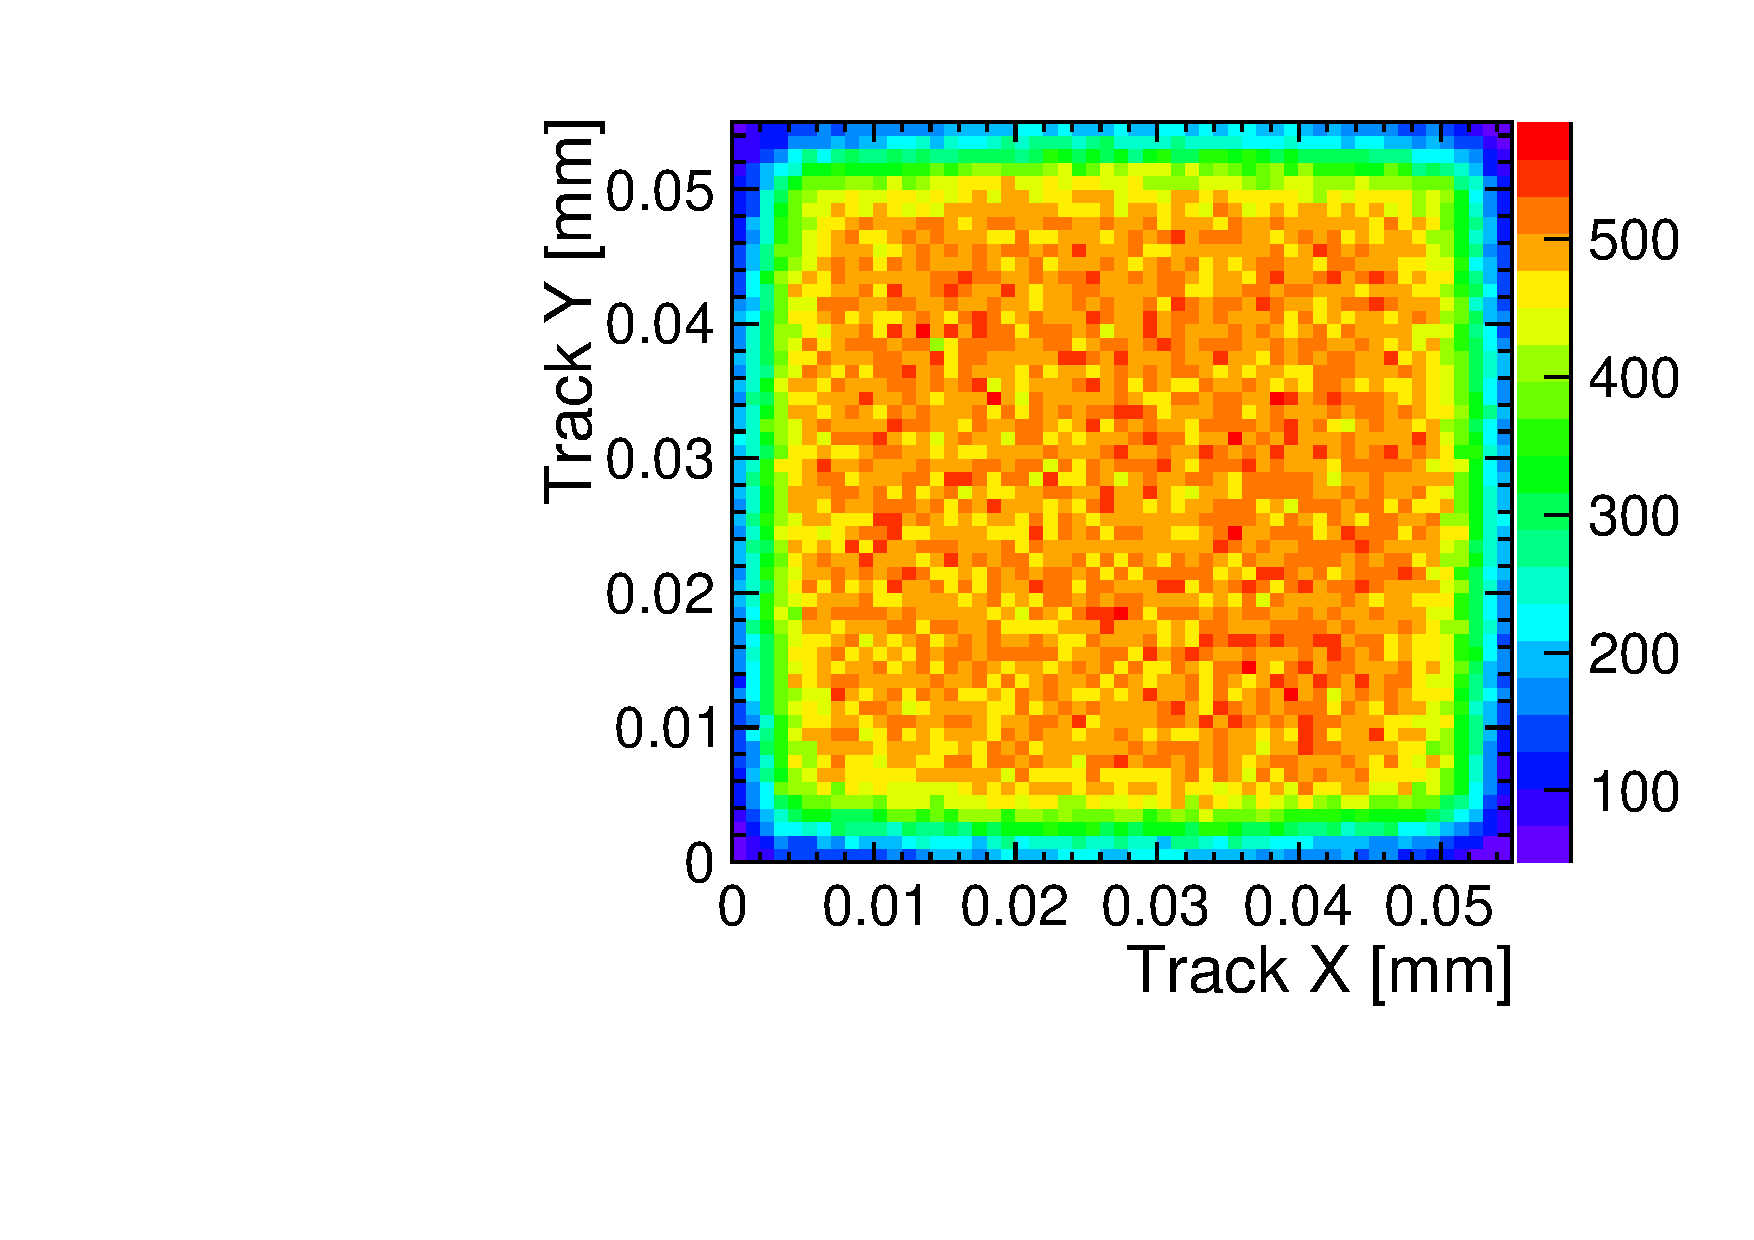
\includegraphics[width=\textwidth]{./figures/TestBeam/TrackPosWPixel_1hit_runW19_G7.pdf}
    \caption{Cluster size 1}
  \end{subfigure} \hfill
  \begin{subfigure}[b]{0.23\textwidth}
    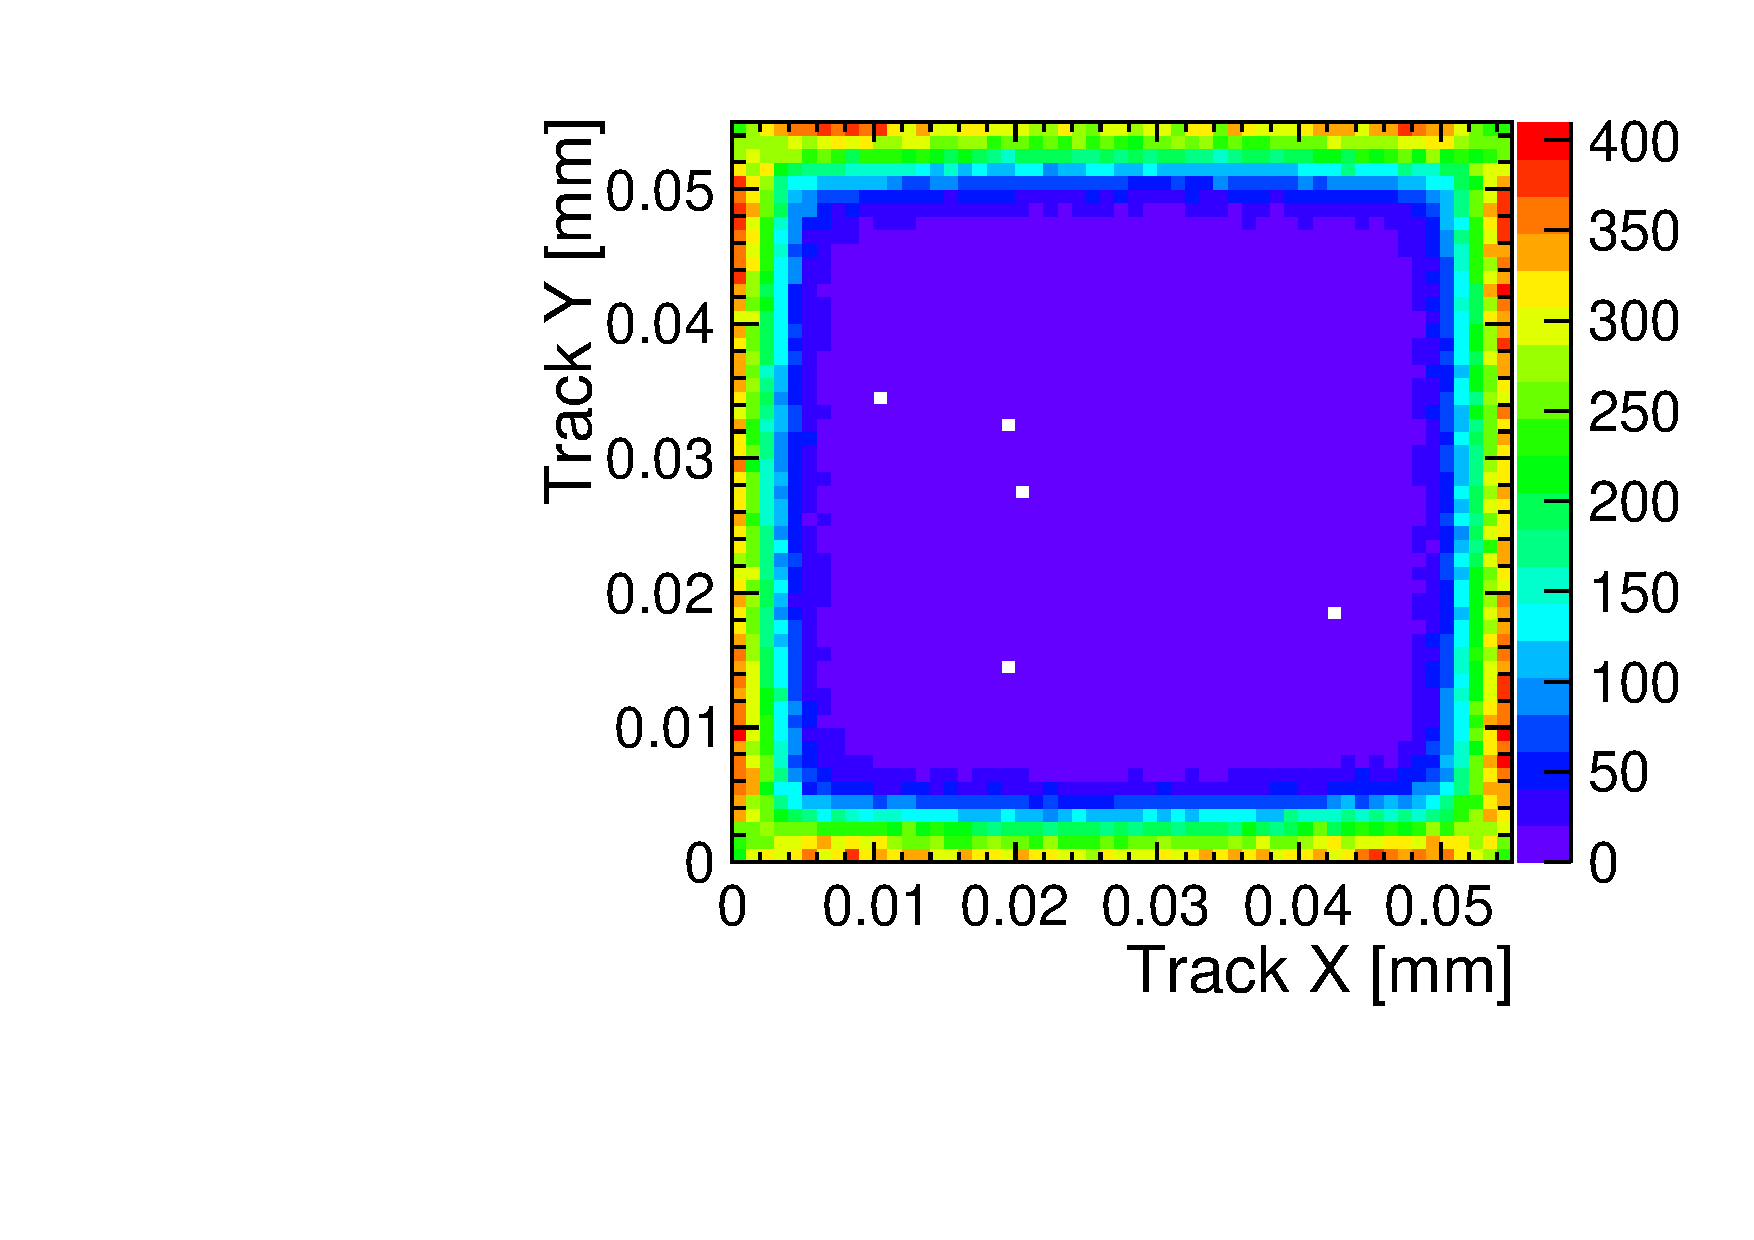
\includegraphics[width=\textwidth]{./figures/TestBeam/TrackPosWPixel_2hit_runW19_G7.pdf}
    \caption{Cluster size 2}
  \end{subfigure} \hfill
  \begin{subfigure}[b]{0.23\textwidth}
    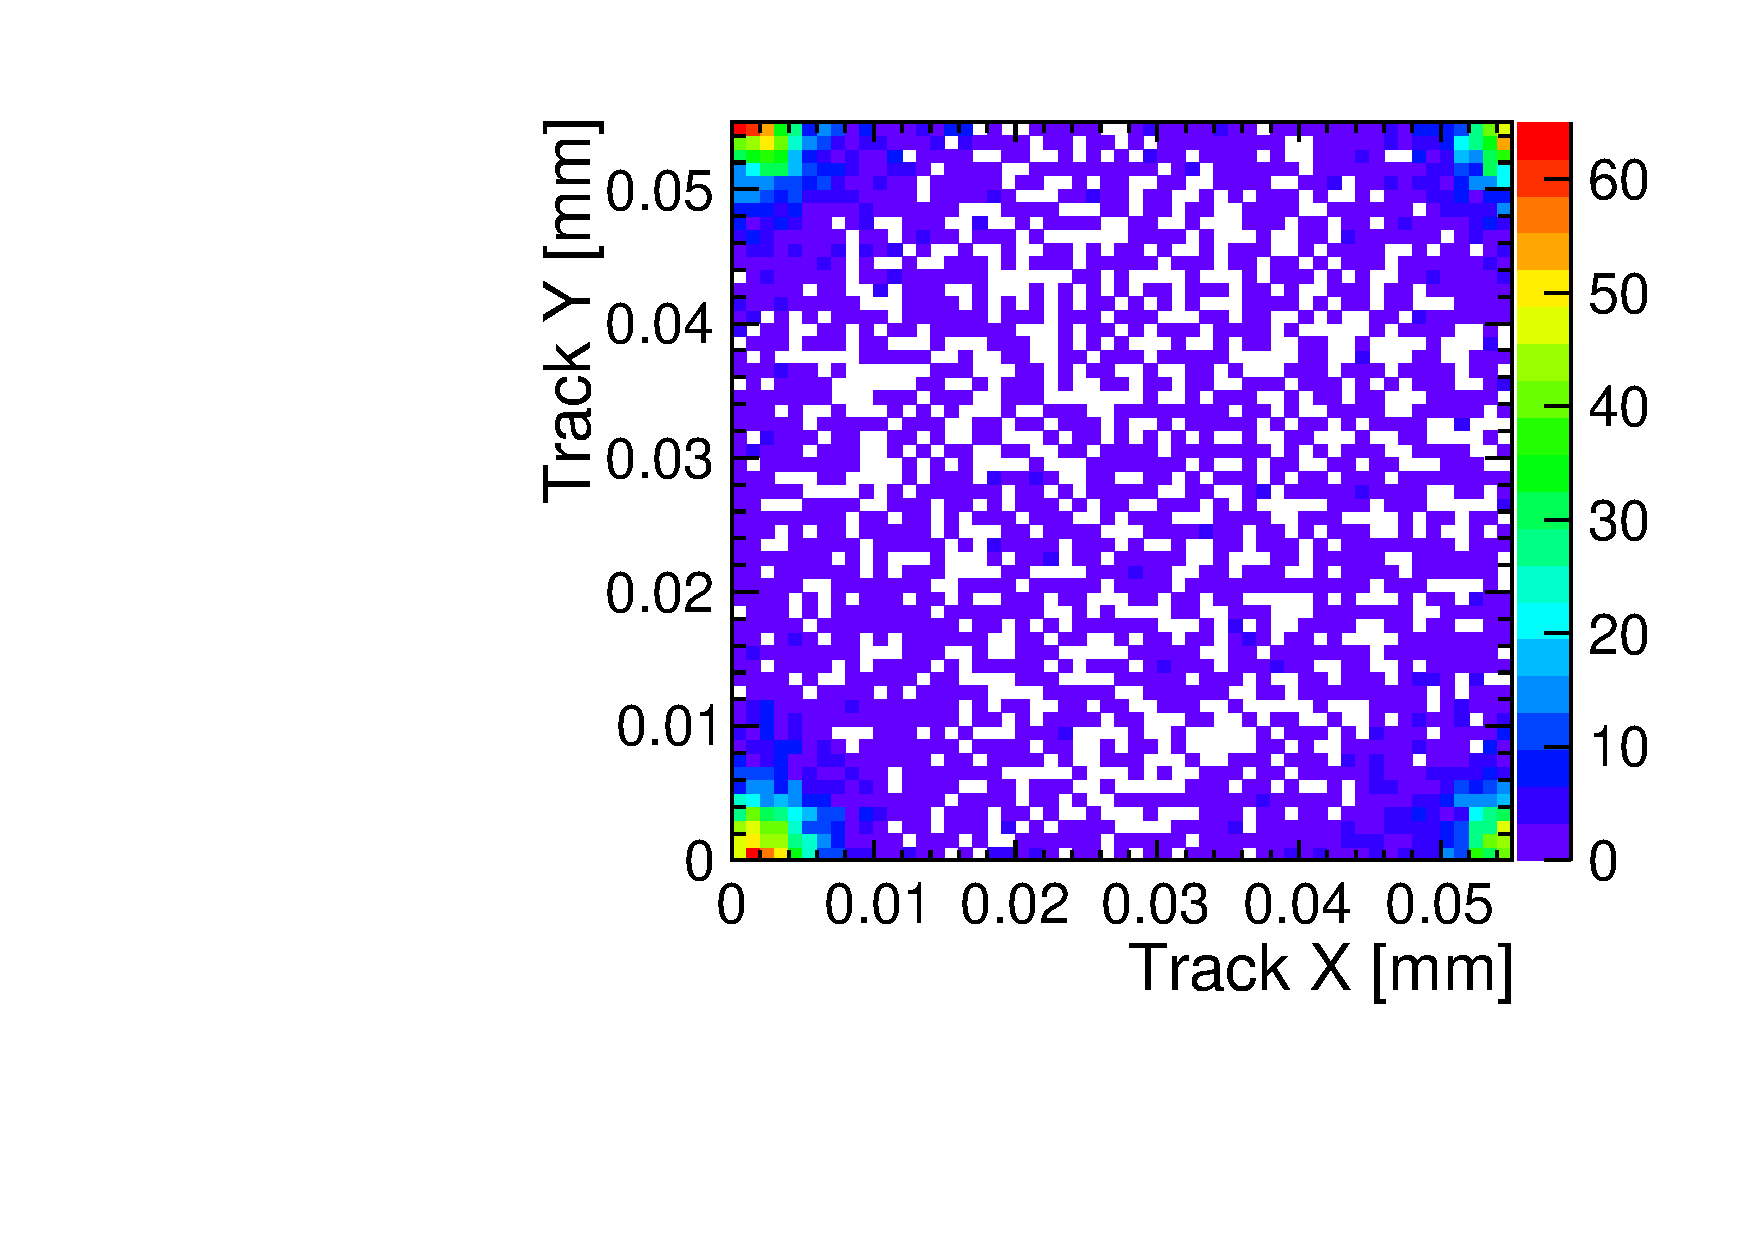
\includegraphics[width=\textwidth]{./figures/TestBeam/TrackPosWPixel_3hit_runW19_G7.pdf}
    \caption{Cluster size 3}
  \end{subfigure} \hfill
  \begin{subfigure}[b]{0.23\textwidth}
    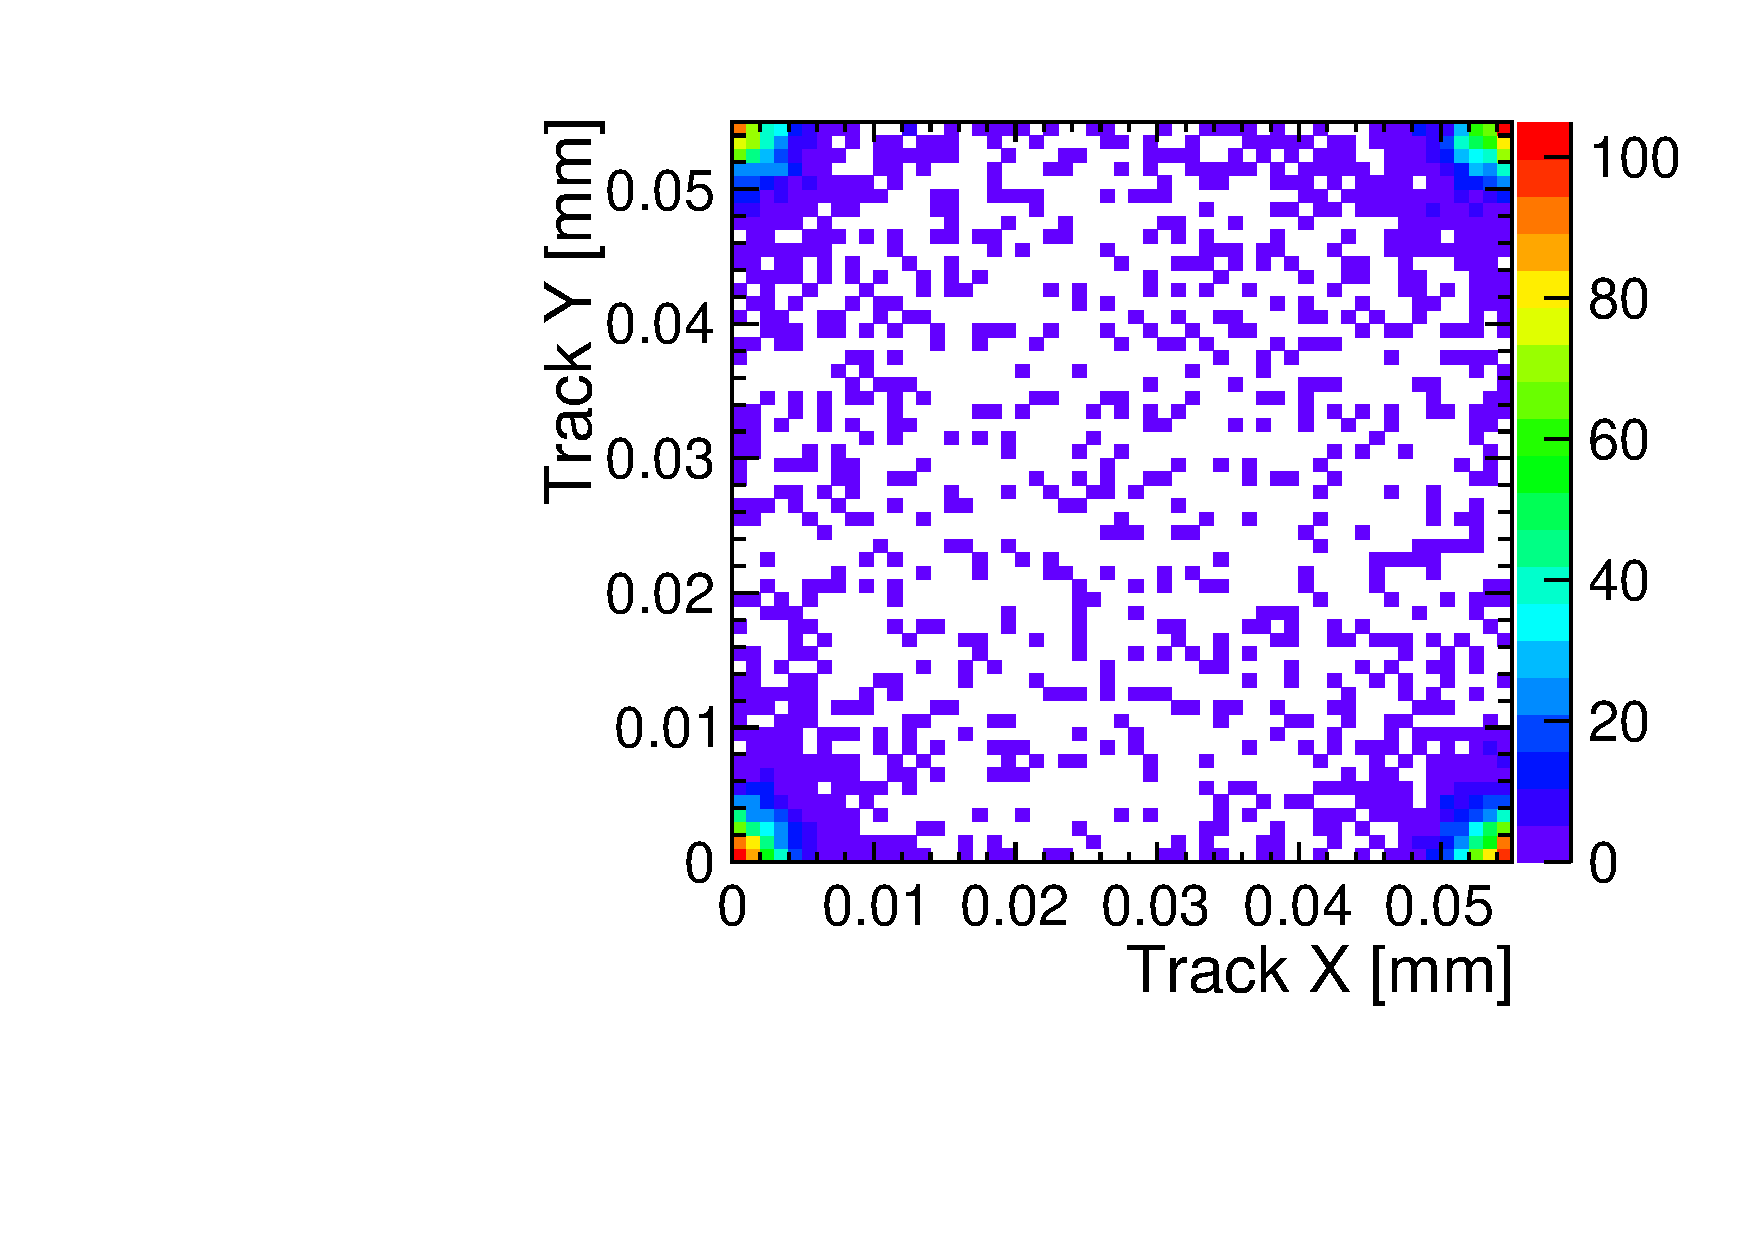
\includegraphics[width=\textwidth]{./figures/TestBeam/TrackPosWPixel_4hit_runW19_G7.pdf}
    \caption{Cluster size 4}
  \end{subfigure}
  \caption{Extrapolated track position within the pixel for 1 to
    4-pixel cluster sizes for a $50\,\micron$ sensor (assembly
    W19\_G7). The assembly is operated at nominal conditions.}
  \label{fig:chargeSharingTrack}
\end{figure}

% \cref{fig:chargeSharing_2PC} compares the track position within the
% pixel for two-pixel clusters in a one-dimensional profile for
% different sensor thicknesses. For thinner sensors, the track position
% should be closer to the edges of the pixels to create two-pixel
% clusters.

% \begin{figure}[htbp] 
%   \centering
%   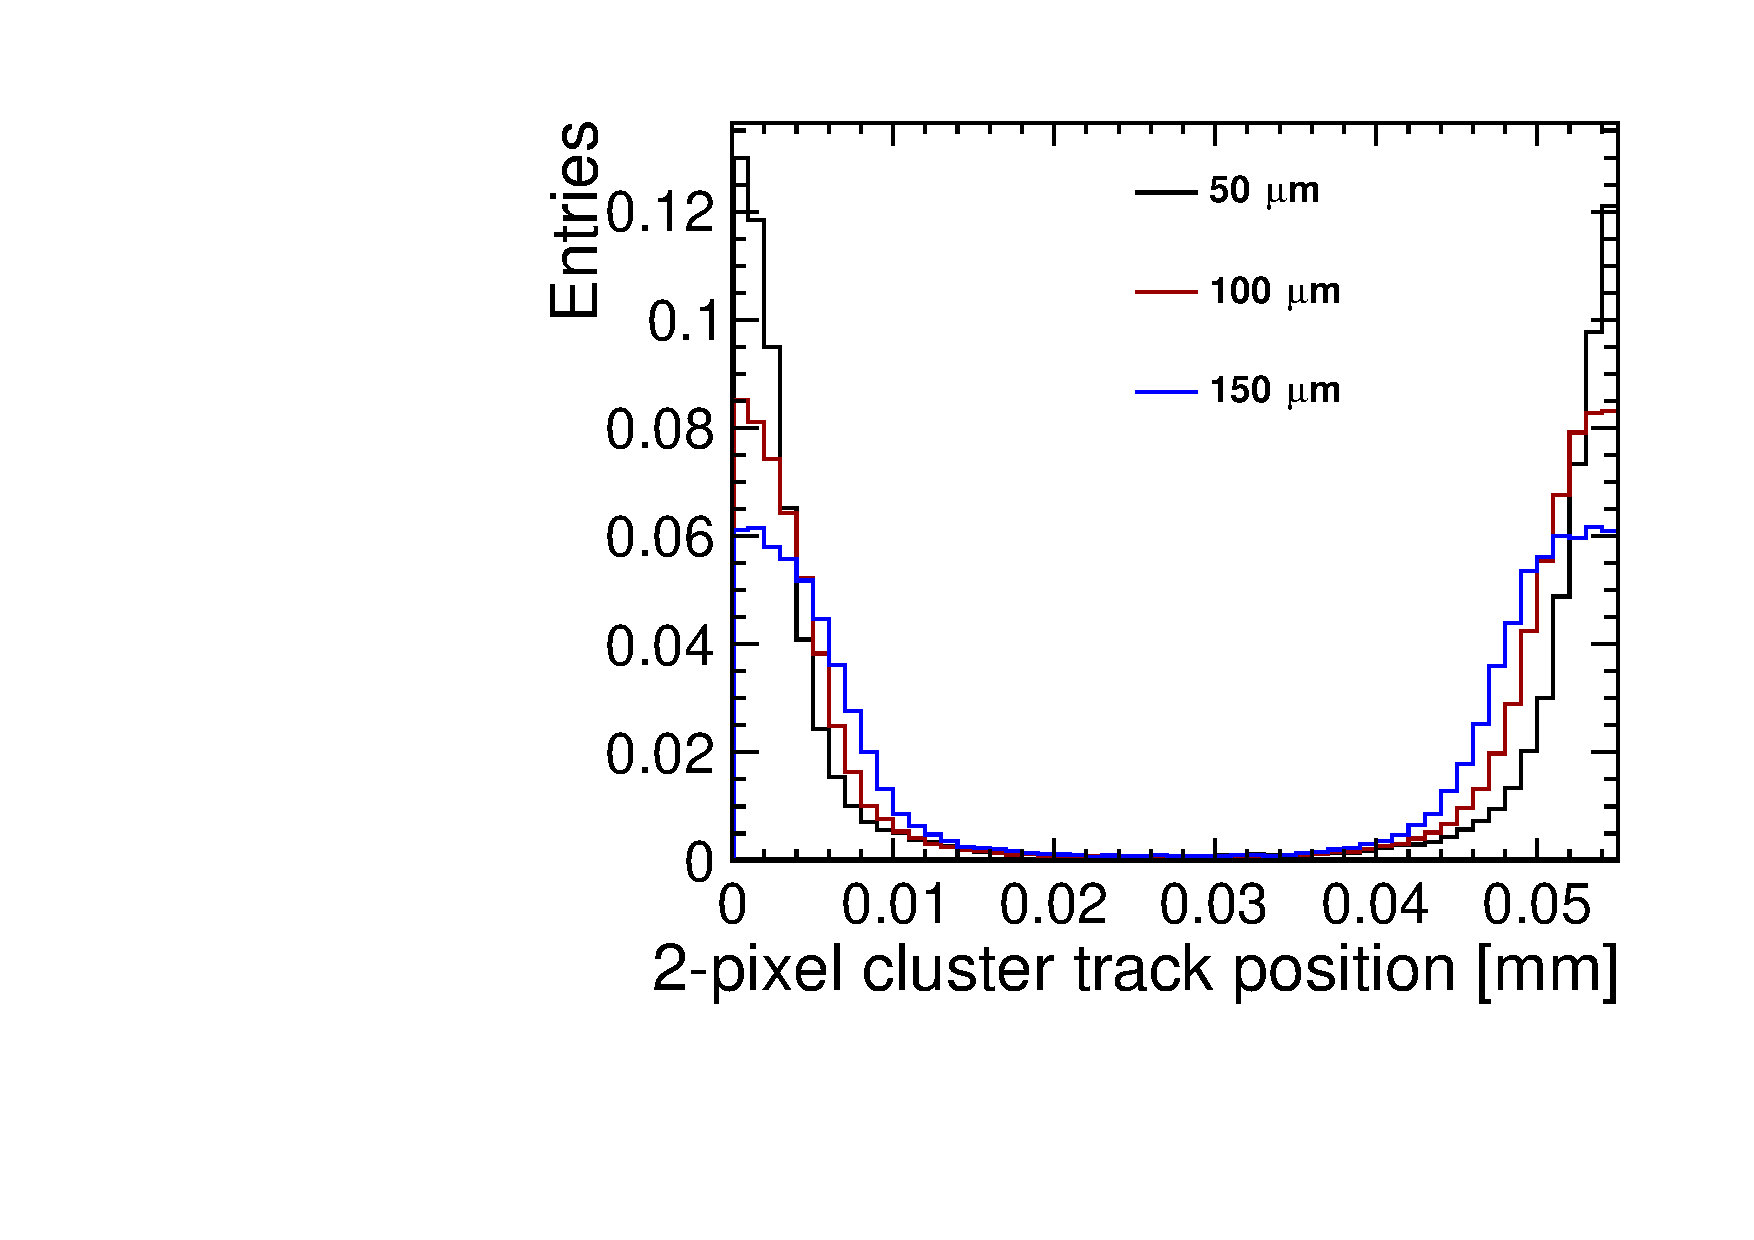
\includegraphics[width=0.5\textwidth]{./figures/TestBeam/chargeSharing_2pixel_clusters.pdf}
%   \caption{Track position within the pixel for tracks leading to
%     two-pixel clusters for different sensor thicknesses (the
%     histograms are scaled to have a unit area).}
%   \label{fig:chargeSharing_2PC}
% \end{figure}


\subsection{Single-point resolution}

From the test-beam data, the residuals are calculated by comparing the
reconstructed hit position with the extrapolated track position
obtained by the telescope. This residual combines in quadrature the
single-point (or hit) and the track resolutions:

\begin{equation}
  \sigma_{\mathrm{residual}}^{2}=\sigma_{\mathrm{hit}}^{2}+\sigma_{\mathrm{track}}^{2} .
  \label{eq:residualEq}
\end{equation}

In the following, the tracking resolution of $\sim2\,\micron$ is not
unfolded from the residual measurements presented (see
\cref{sec:TrackResOnDUT}).
% For the estimation
% of the single-point resolution, the tracking resolution of
% $\sim2\,\micron$ at the SPS test beam should be unfolded
% (c.f.~\cref{ch:Telescope}).

The residuals depend on the cluster sizes since the reconstructed hit
position takes into account the number of the hit pixels in a cluster
and the charge information in each pixel. \cref{fig:residuals_cluSize}
illustrates the residuals for a $50\,\micron$ thick sensor (assembly
W19\_G7) for different cluster sizes. For single-pixel clusters, the
hit position corresponds to the geometric center of the pixel and
therefore the charge information can not improve the resolution. For
multi-pixel clusters, the $\eta$-correction method (see
\cref{sec:EtaCorrection}) provides a more accurate interpolation of
the hit position using the charge deposition (TOT) in the pixels hit
and improves the resolution.


\begin{figure}[htbp] \centering
  \begin{subfigure}[b]{0.23\textwidth}
    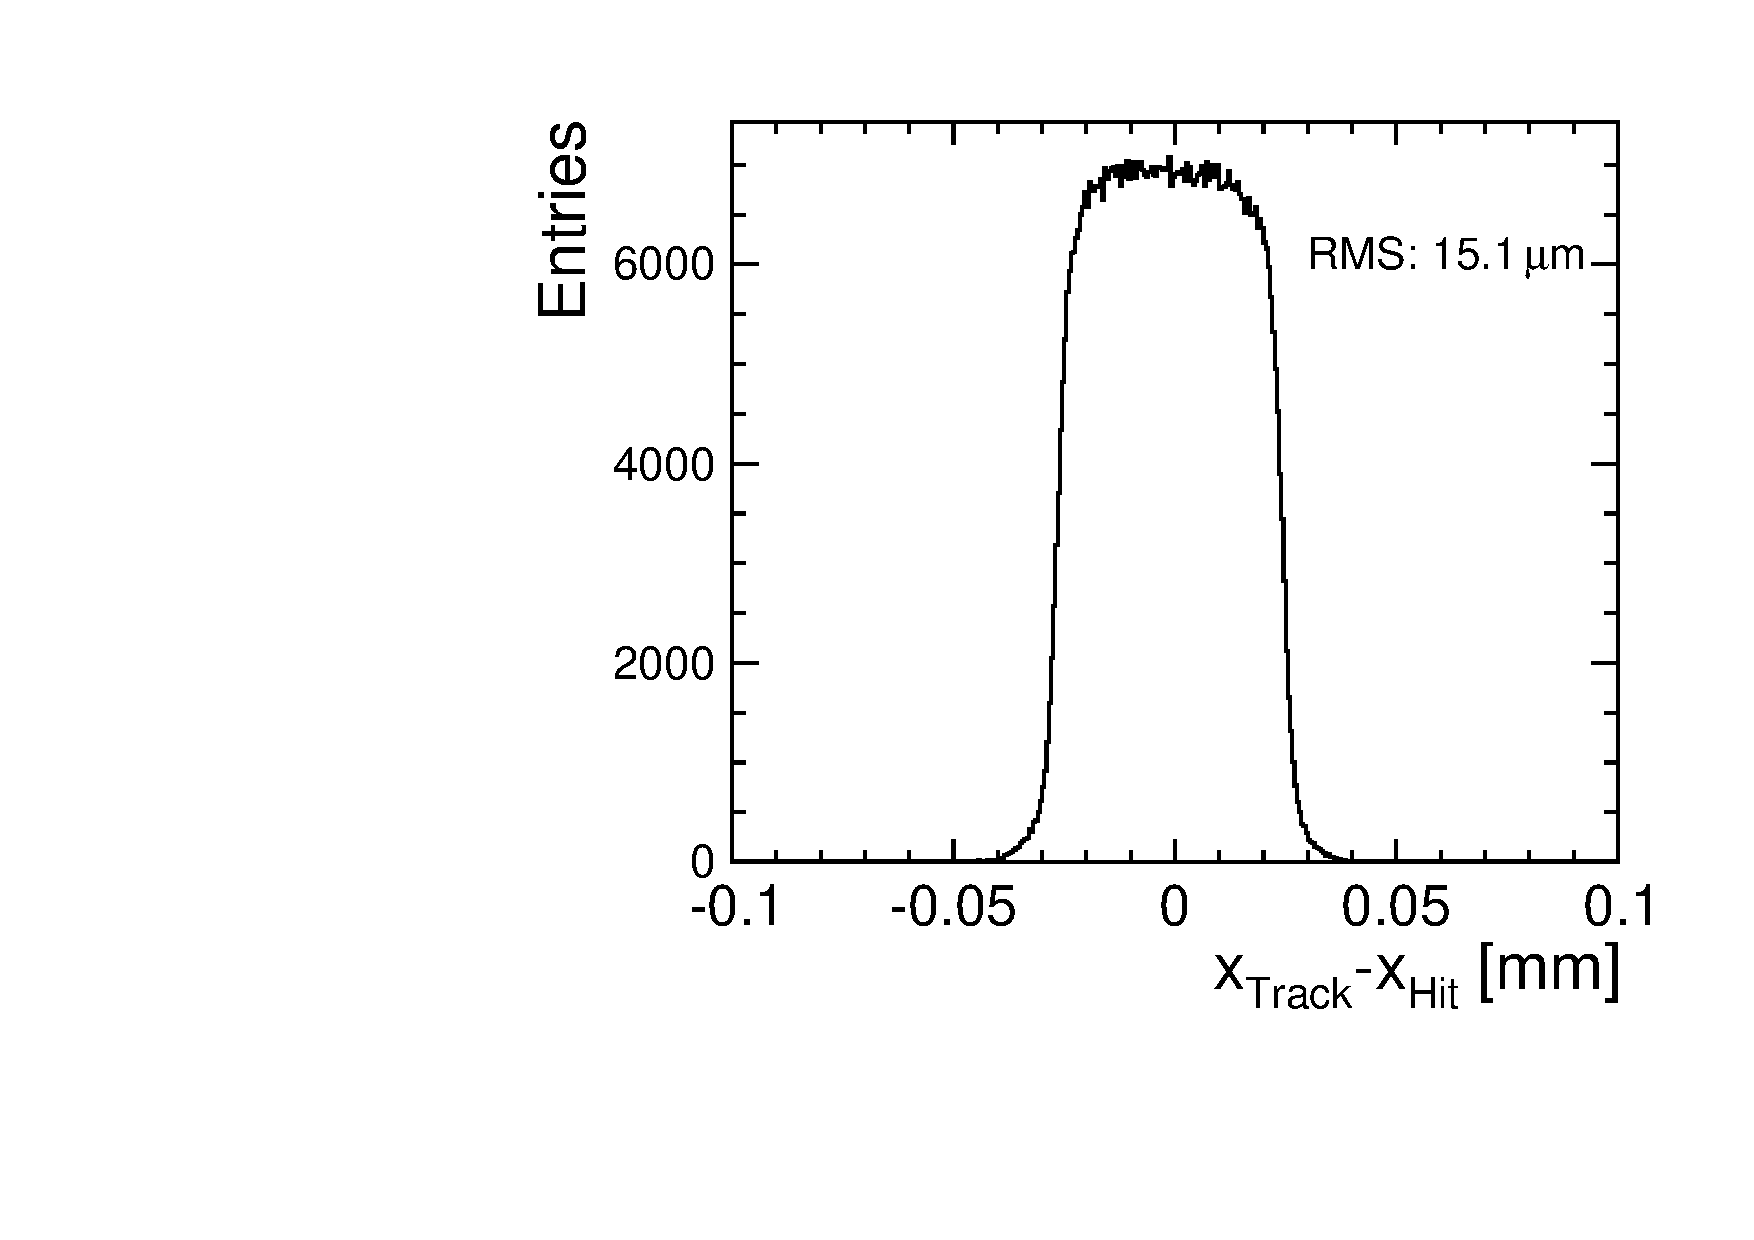
\includegraphics[width=\textwidth]{./figures/TestBeam/residual_1hit_W19_G7.pdf}
    \caption{Cluster size 1}
  \end{subfigure} \hfill
  \begin{subfigure}[b]{0.23\textwidth}
    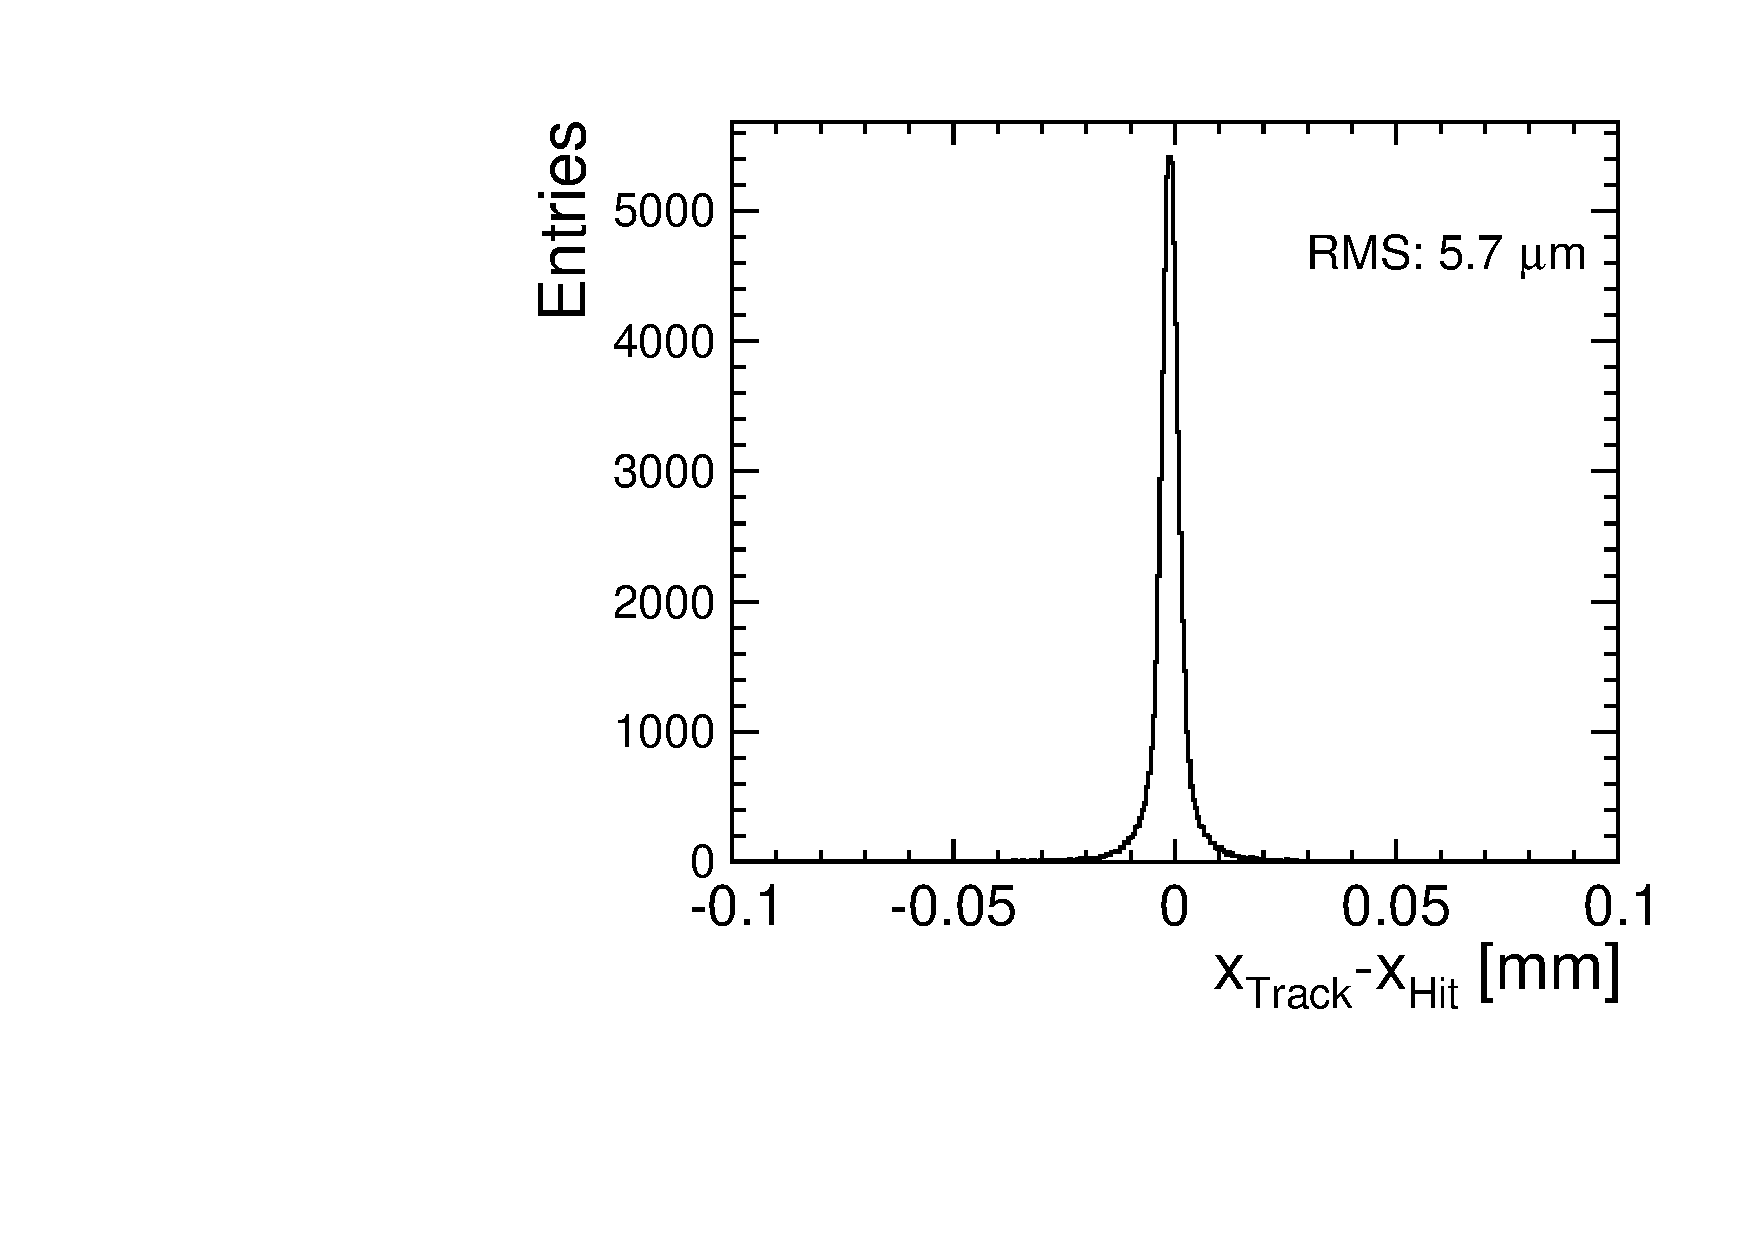
\includegraphics[width=\textwidth]{./figures/TestBeam/residual_2hit_W19_G7.pdf}
    \caption{Cluster size 2}
  \end{subfigure} \hfill
  \begin{subfigure}[b]{0.23\textwidth}
    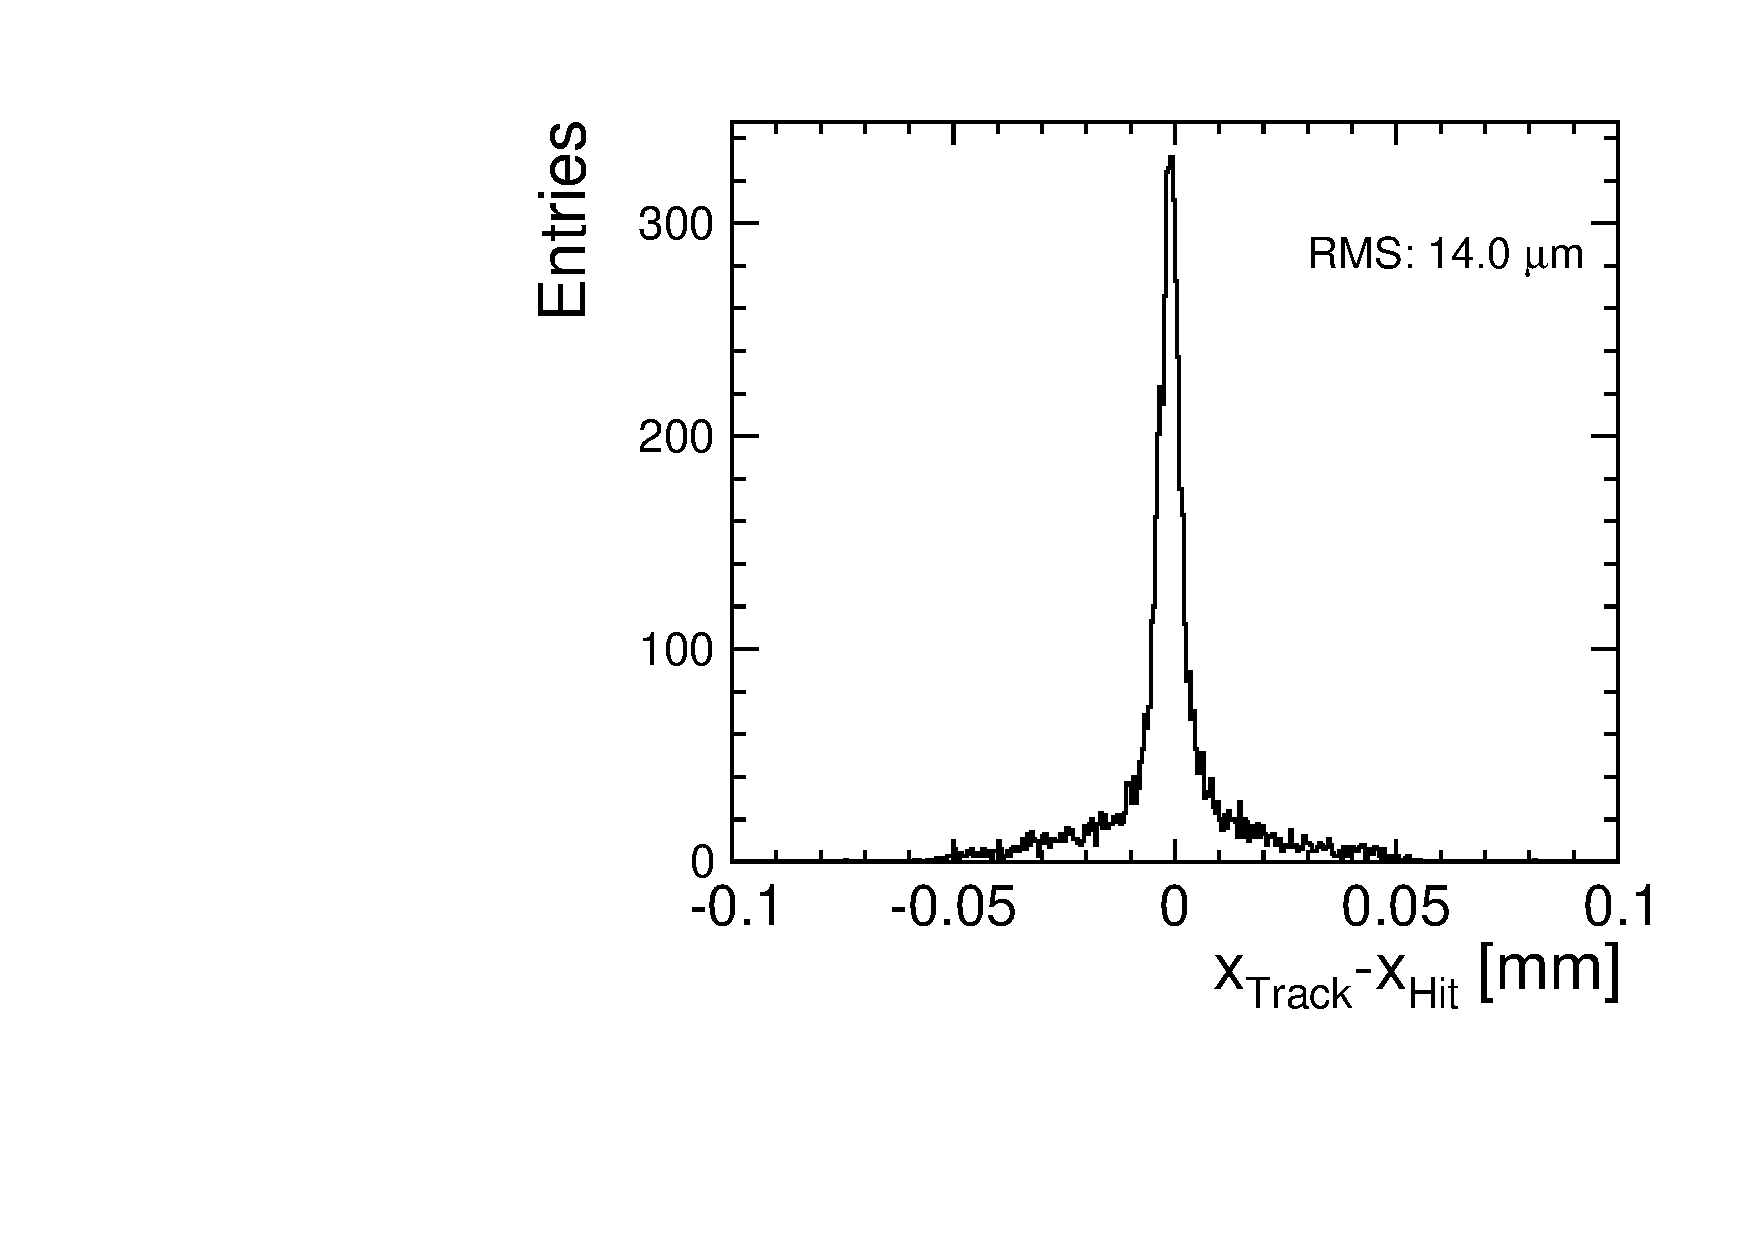
\includegraphics[width=\textwidth]{./figures/TestBeam/residual_3hit_W19_G7.pdf}
    \caption{Cluster size 3}
  \end{subfigure} \hfill
  \begin{subfigure}[b]{0.23\textwidth}
    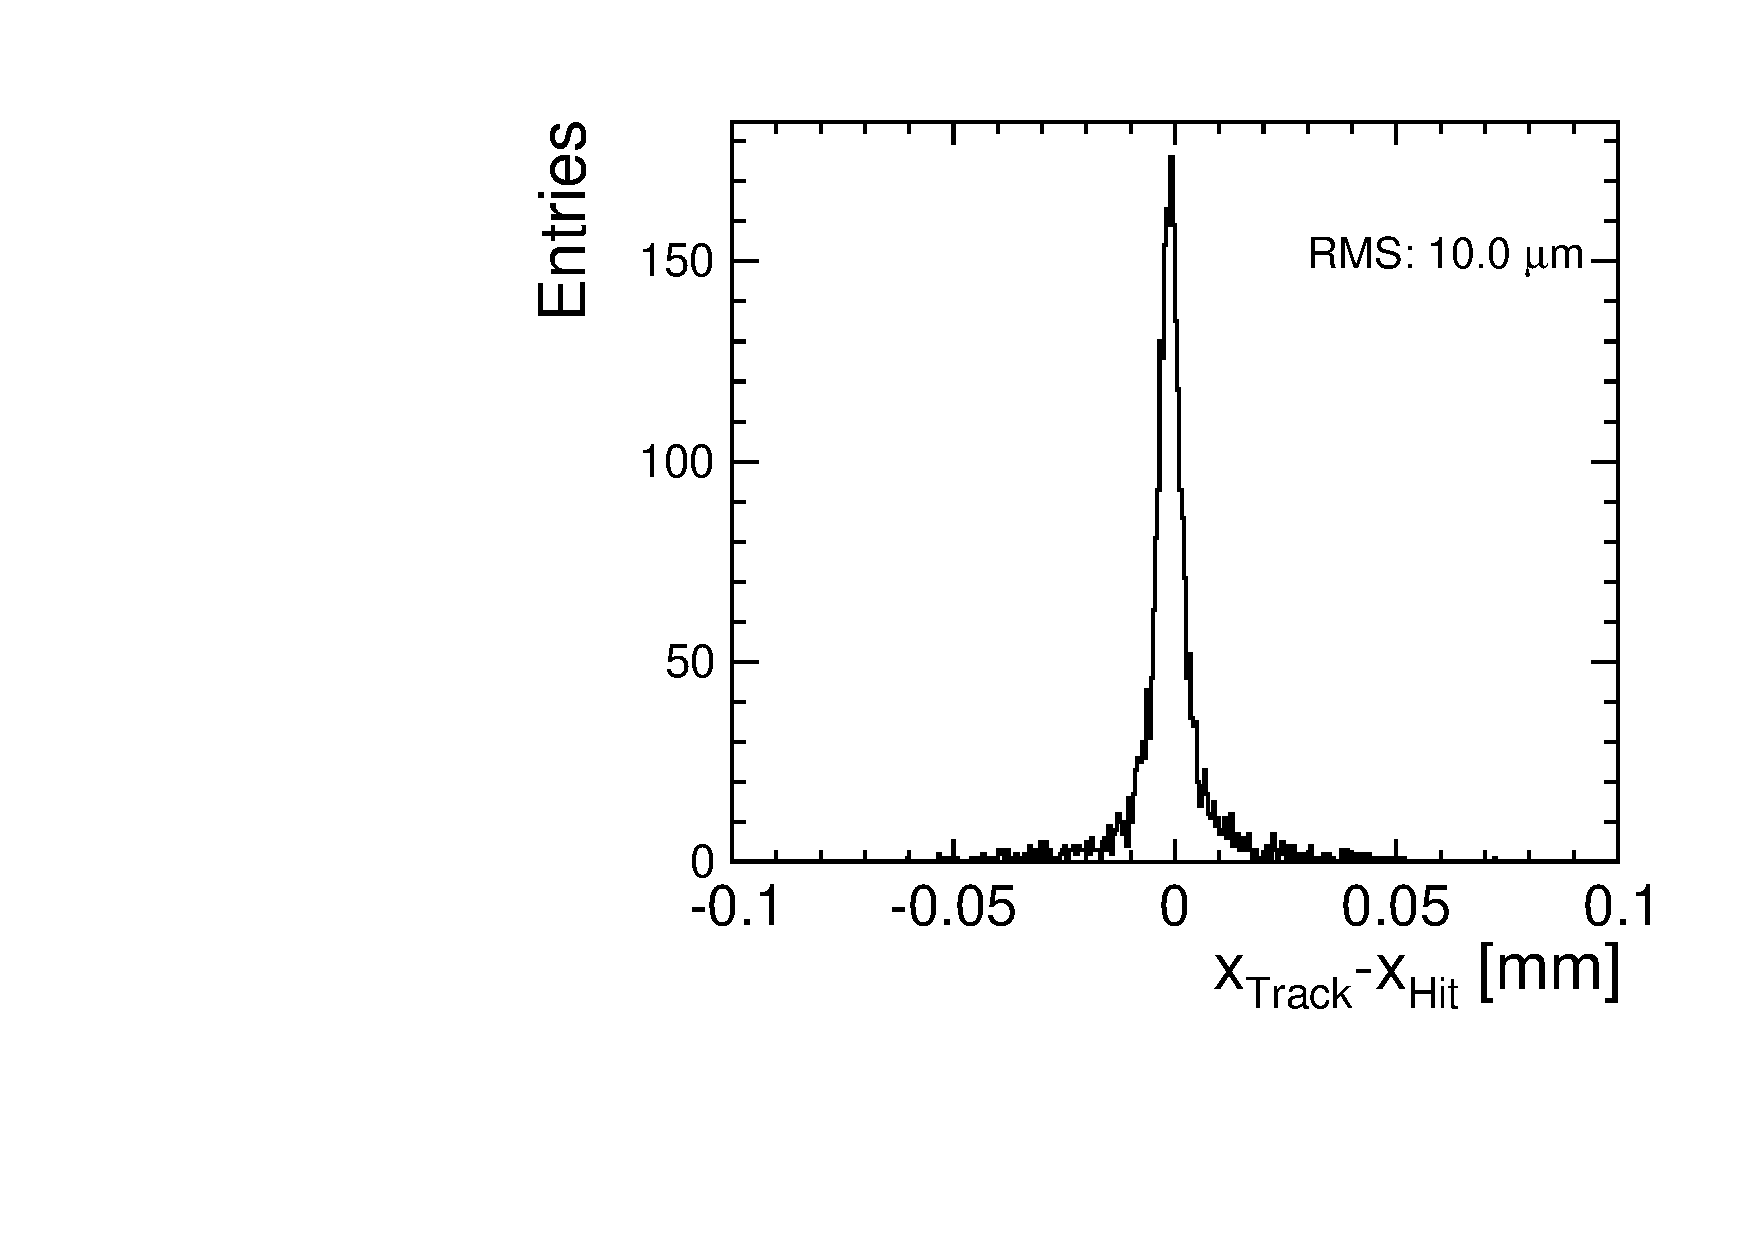
\includegraphics[width=\textwidth]{./figures/TestBeam/residual_4hit_W19_G7.pdf}
    \caption{Cluster size 4}
  \end{subfigure}
  \caption{The residuals for a $50\,\micron$ thick sensor (assembly
    W19\_G7) for different cluster sizes: (a) Cluster size 1
    ($1\times1$), (b) Cluster size 2 ($2\times1$), (c) Cluster size 3
    ($2\times2$) and (d) Cluster size 4 ($2\times2$).}
  \label{fig:residuals_cluSize}
\end{figure}

The overall residual is defined by the RMS of the residual of all
tracks combined. The distribution of the residuals for different
sensor thicknesses operated at nominal conditions in simulation and
data is shown in \cref{fig:G4_simu_data_Residuals}. The wider
component in the residual distributions corresponds to the
single-pixel clusters. For thicker sensors, the fraction of
multi-pixel clusters increases. This leads to a higher fraction of
more precisely reconstructed hits and therefore the residual
distribution gets narrower. There is a good agreement between
simulation and data.

\begin{figure}[htbp] \centering
  \begin{subfigure}[b]{0.3\textwidth}
    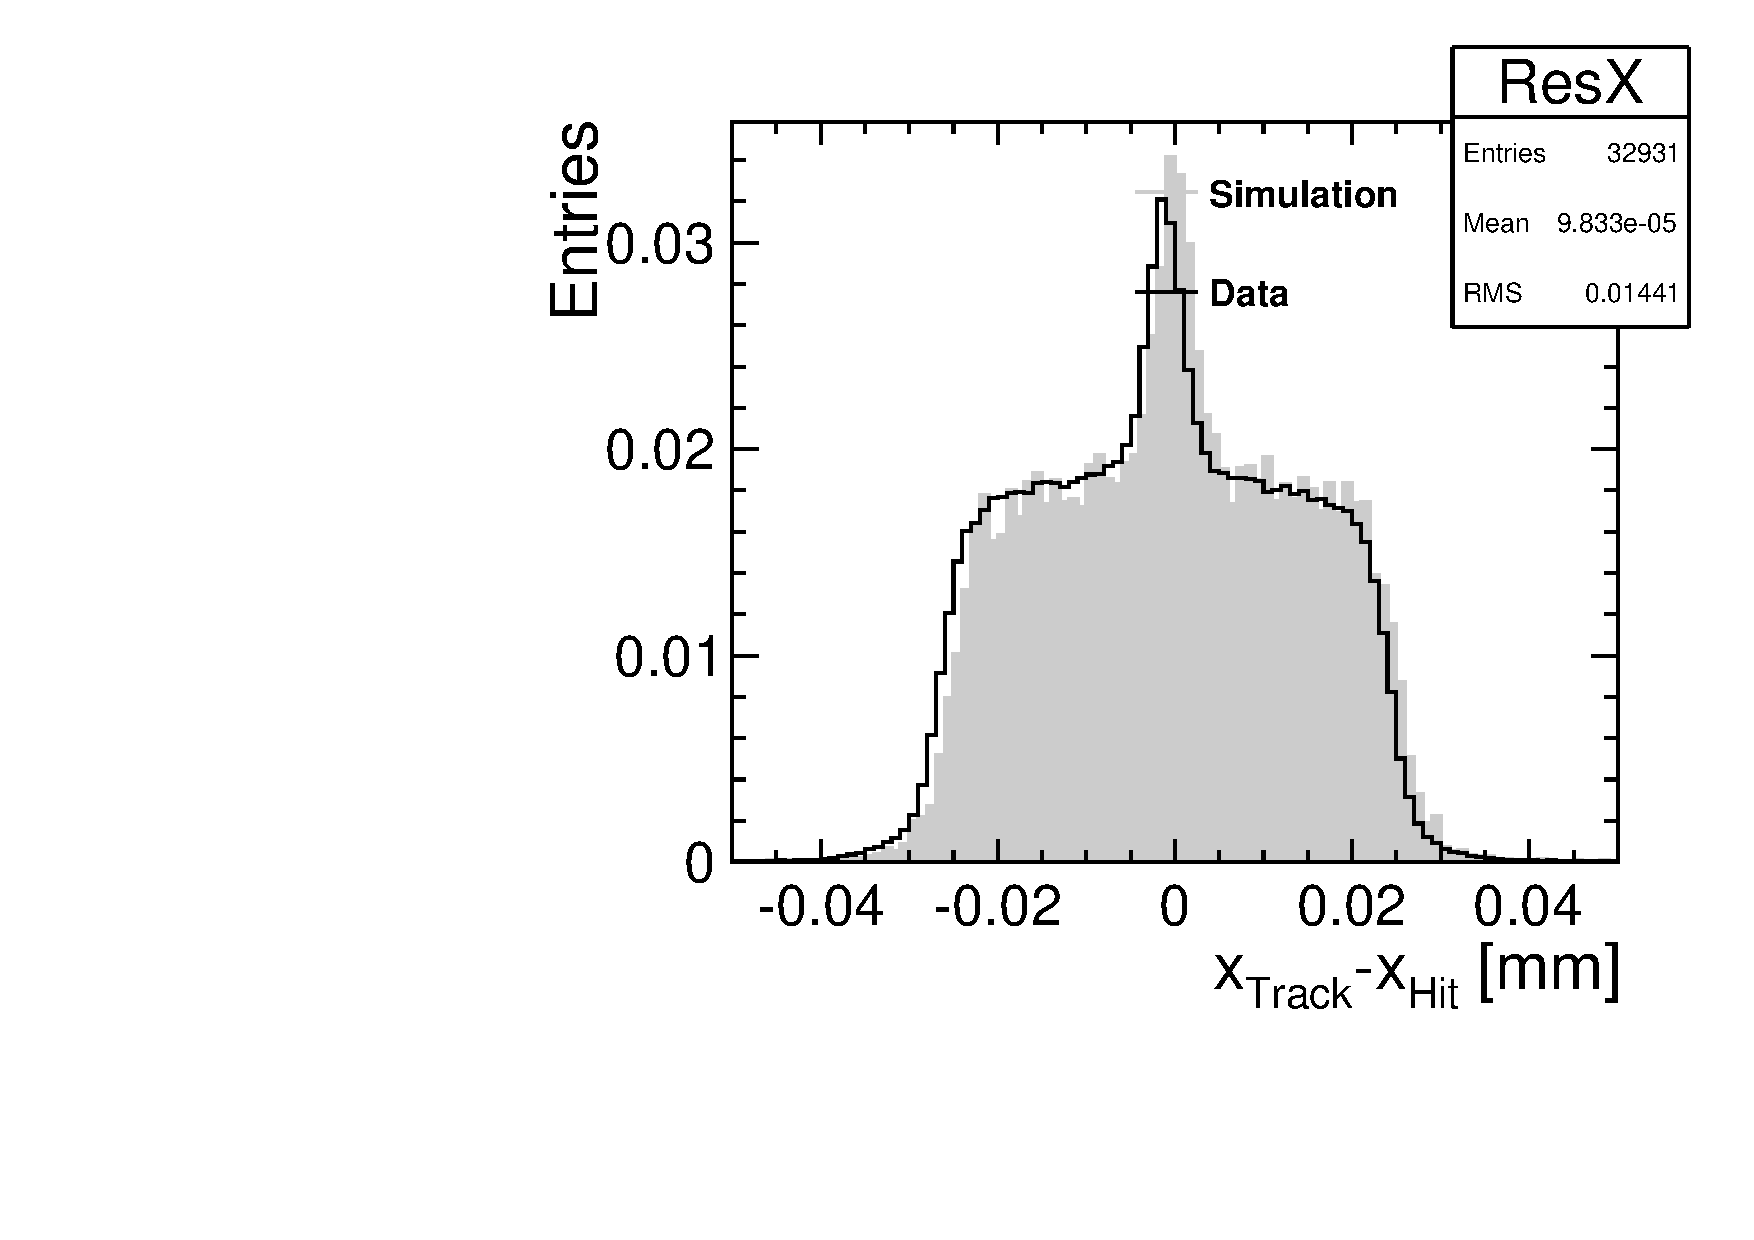
\includegraphics[width=\textwidth]{figures/TestBeam/50micron_resX.pdf}
    \caption{$50\,\micron$}
  \end{subfigure} \hfill
  \begin{subfigure}[b]{0.3\textwidth}
    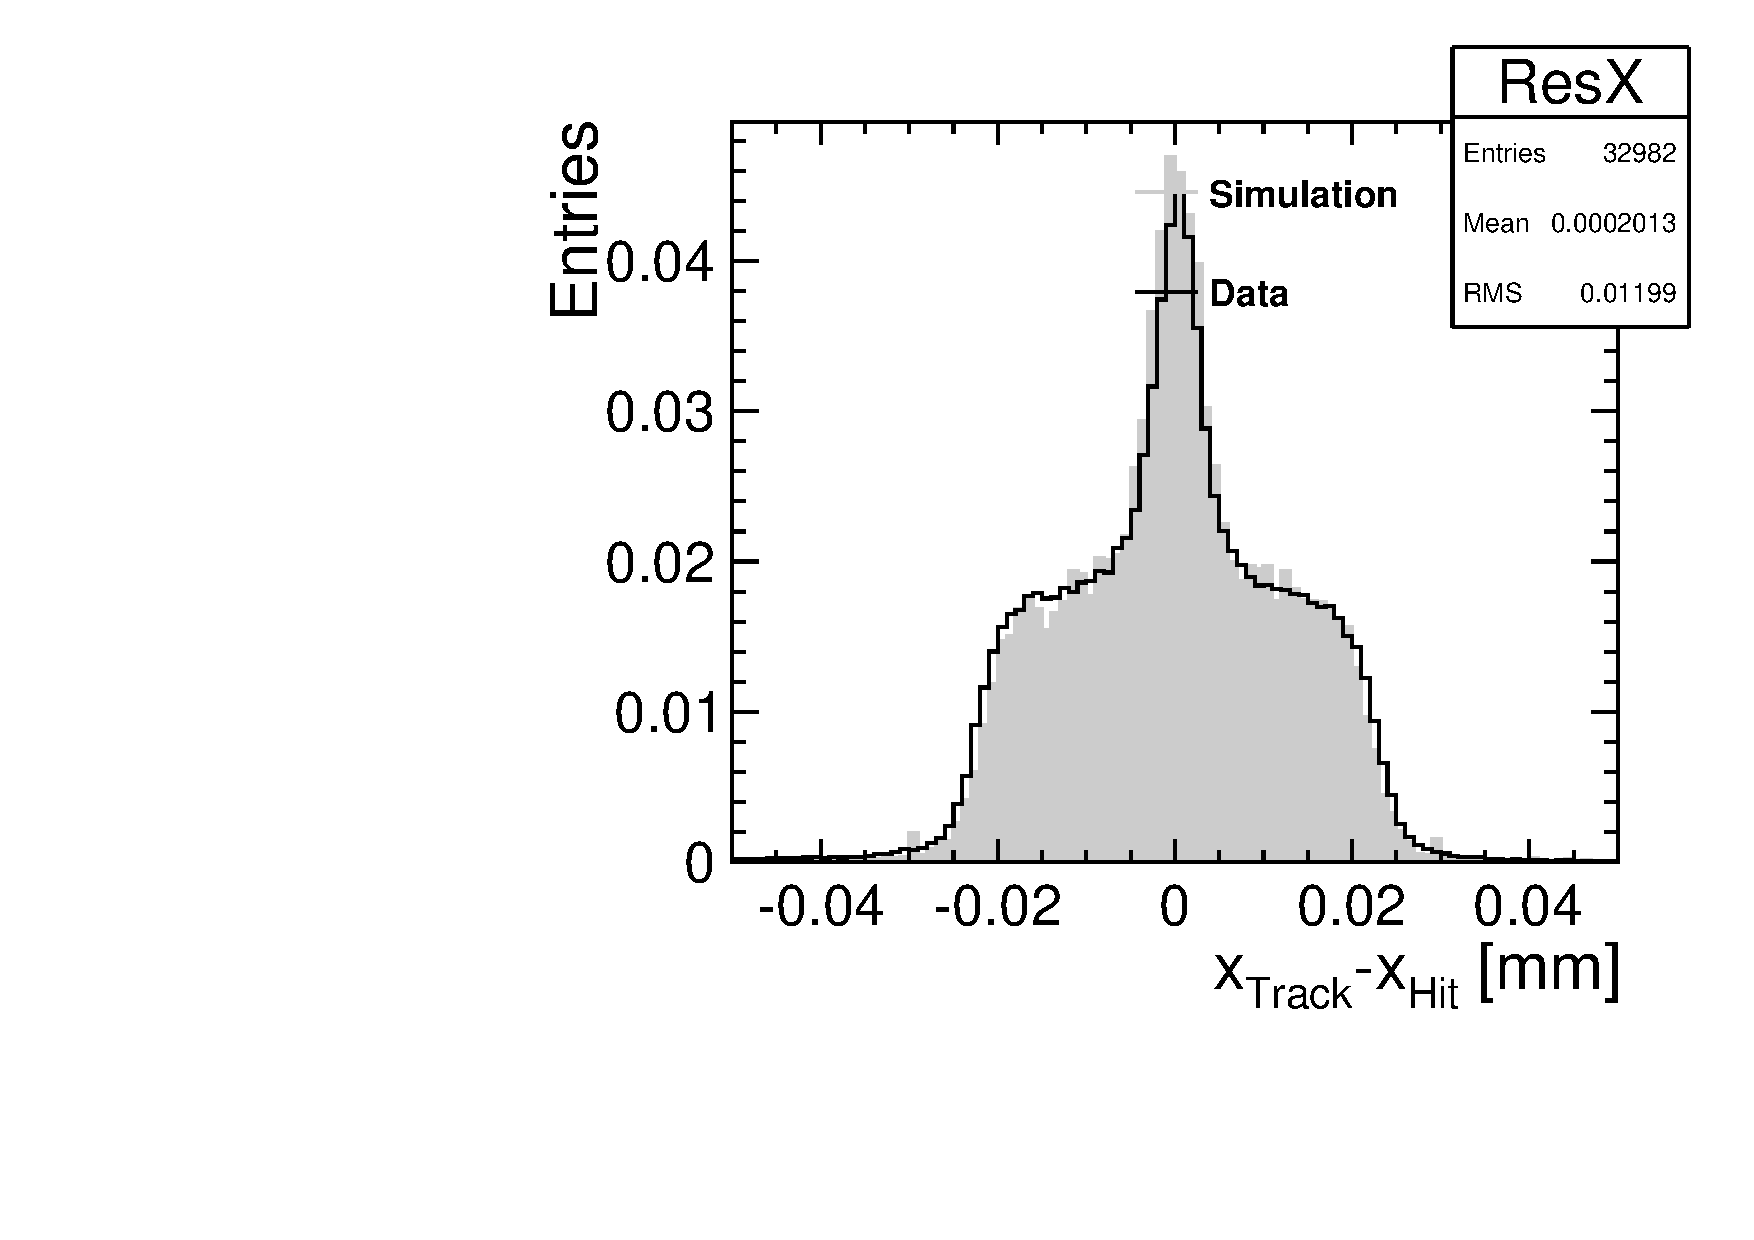
\includegraphics[width=\textwidth]{figures/TestBeam/100micron_resX.pdf}
    \caption{$100\,\micron$}
  \end{subfigure} \hfill
  \begin{subfigure}[b]{0.3\textwidth}
    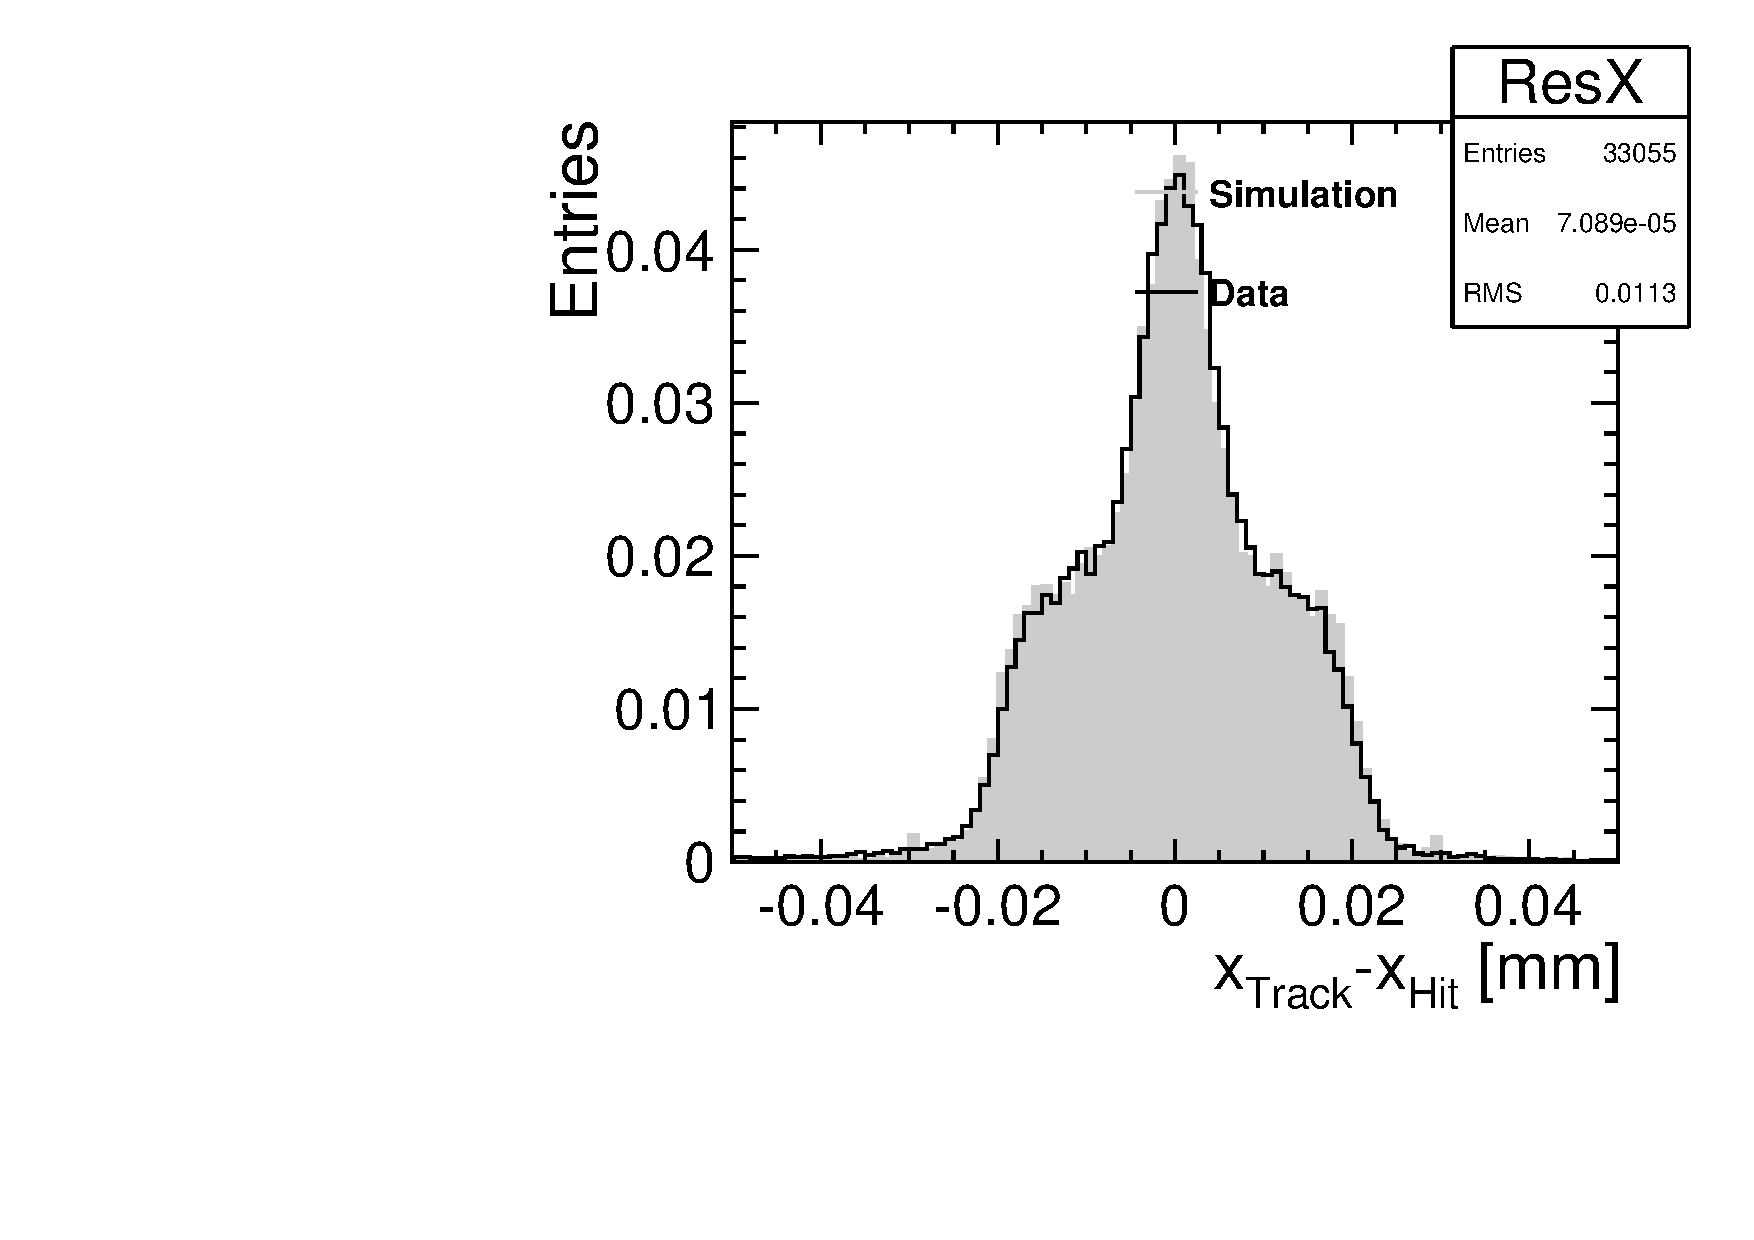
\includegraphics[width=\textwidth]{figures/TestBeam/150micron_resX.pdf}
    \caption{$150\,\micron$}
  \end{subfigure} 
  %% \hfill
  %% \begin{subfigure}[b]{0.23\textwidth}

  %%   \caption{$300\,\micron$ p-in-n}
  %% \end{subfigure}
  \caption{The residual distribution in the x (column) direction in
    simulation and data for the assemblies (a) W19\_G7, (b) W5\_E2 and
    (c) W5\_F1. The assemblies are operated at nominal conditions. The
    histograms are scaled to have unit area.}
  \label{fig:G4_simu_data_Residuals}
\end{figure}

%% \begin{figure}[htbp] \centering
%%   \begin{subfigure}[b]{0.23\textwidth}
%%     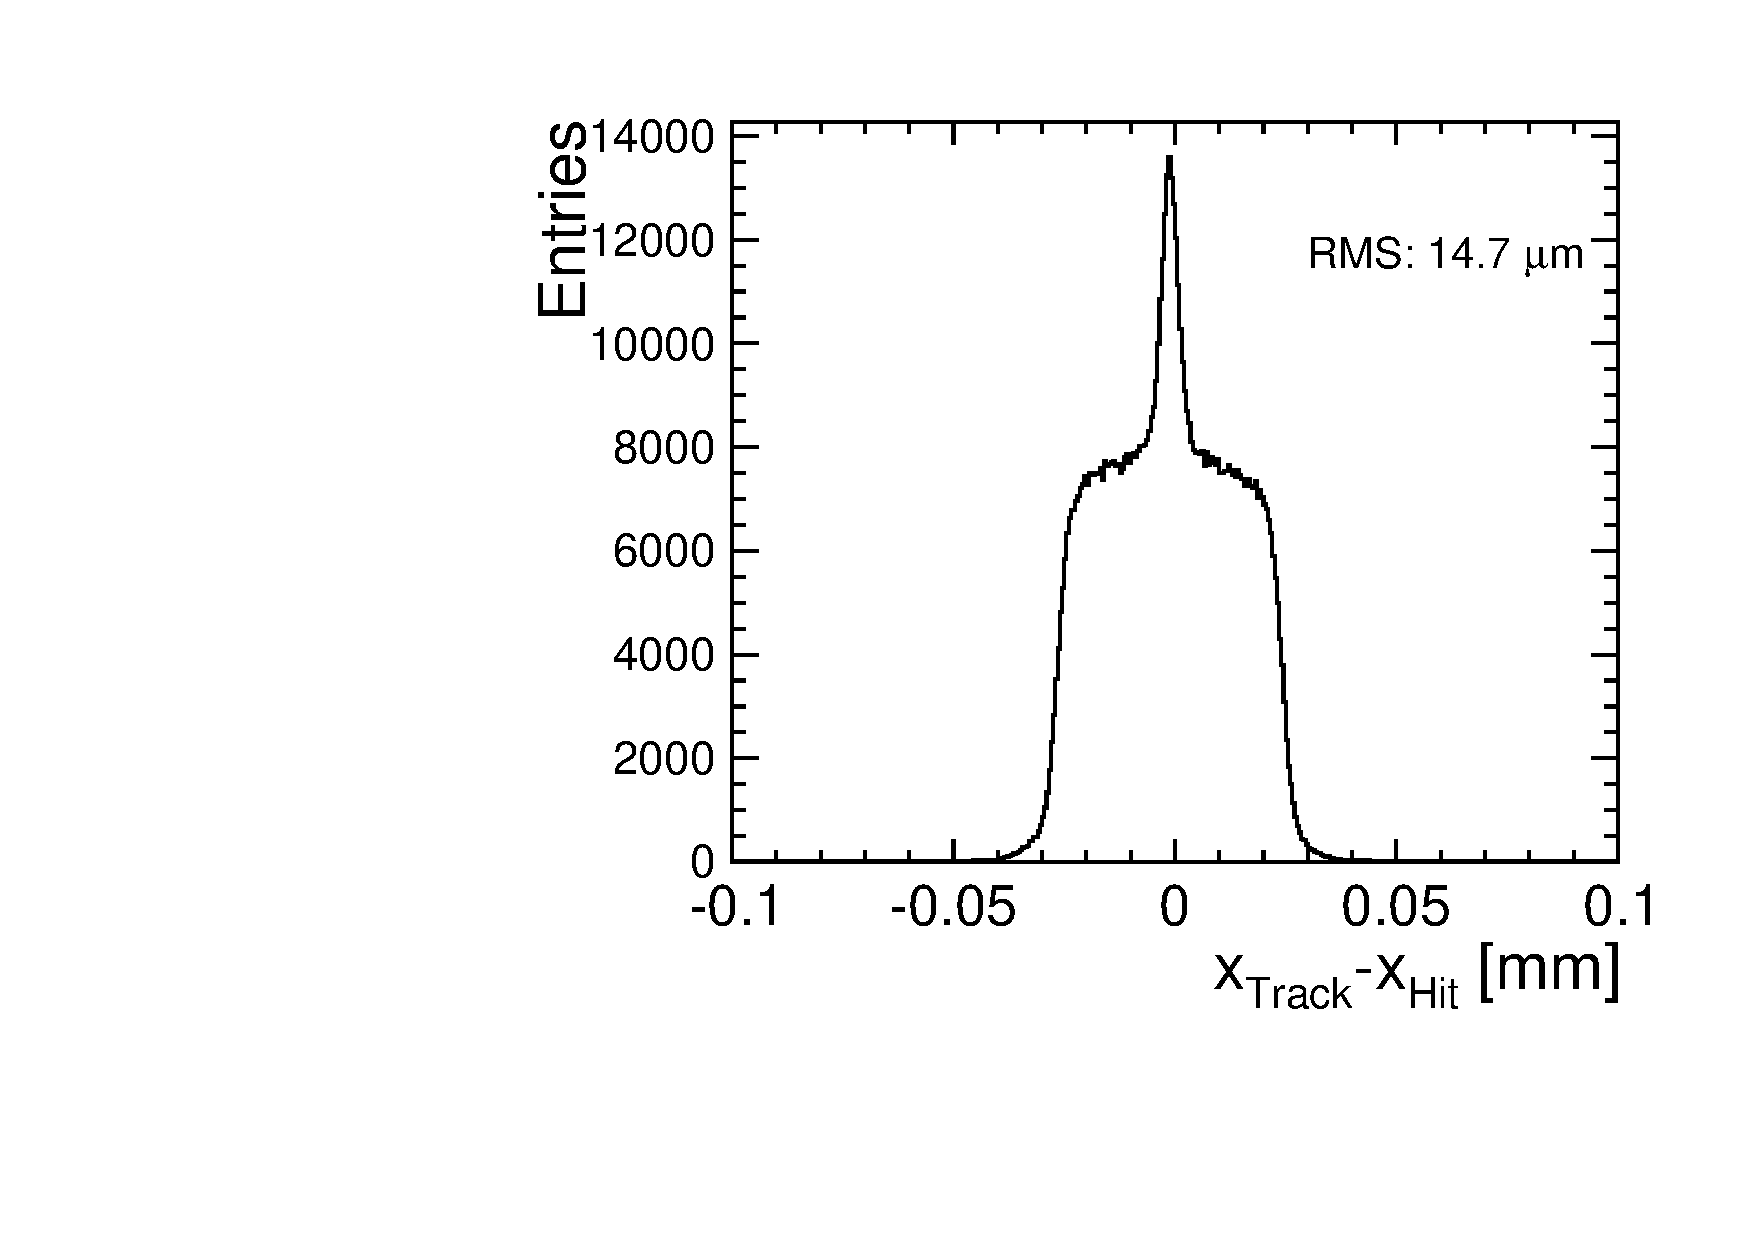
\includegraphics[width=\textwidth]{./figures/TestBeam/residualsHist_W19_C7.pdf}
%%     \caption{$50\,\micron$ sensor}
%%   \end{subfigure} \hfill
%%   \begin{subfigure}[b]{0.23\textwidth}
%%     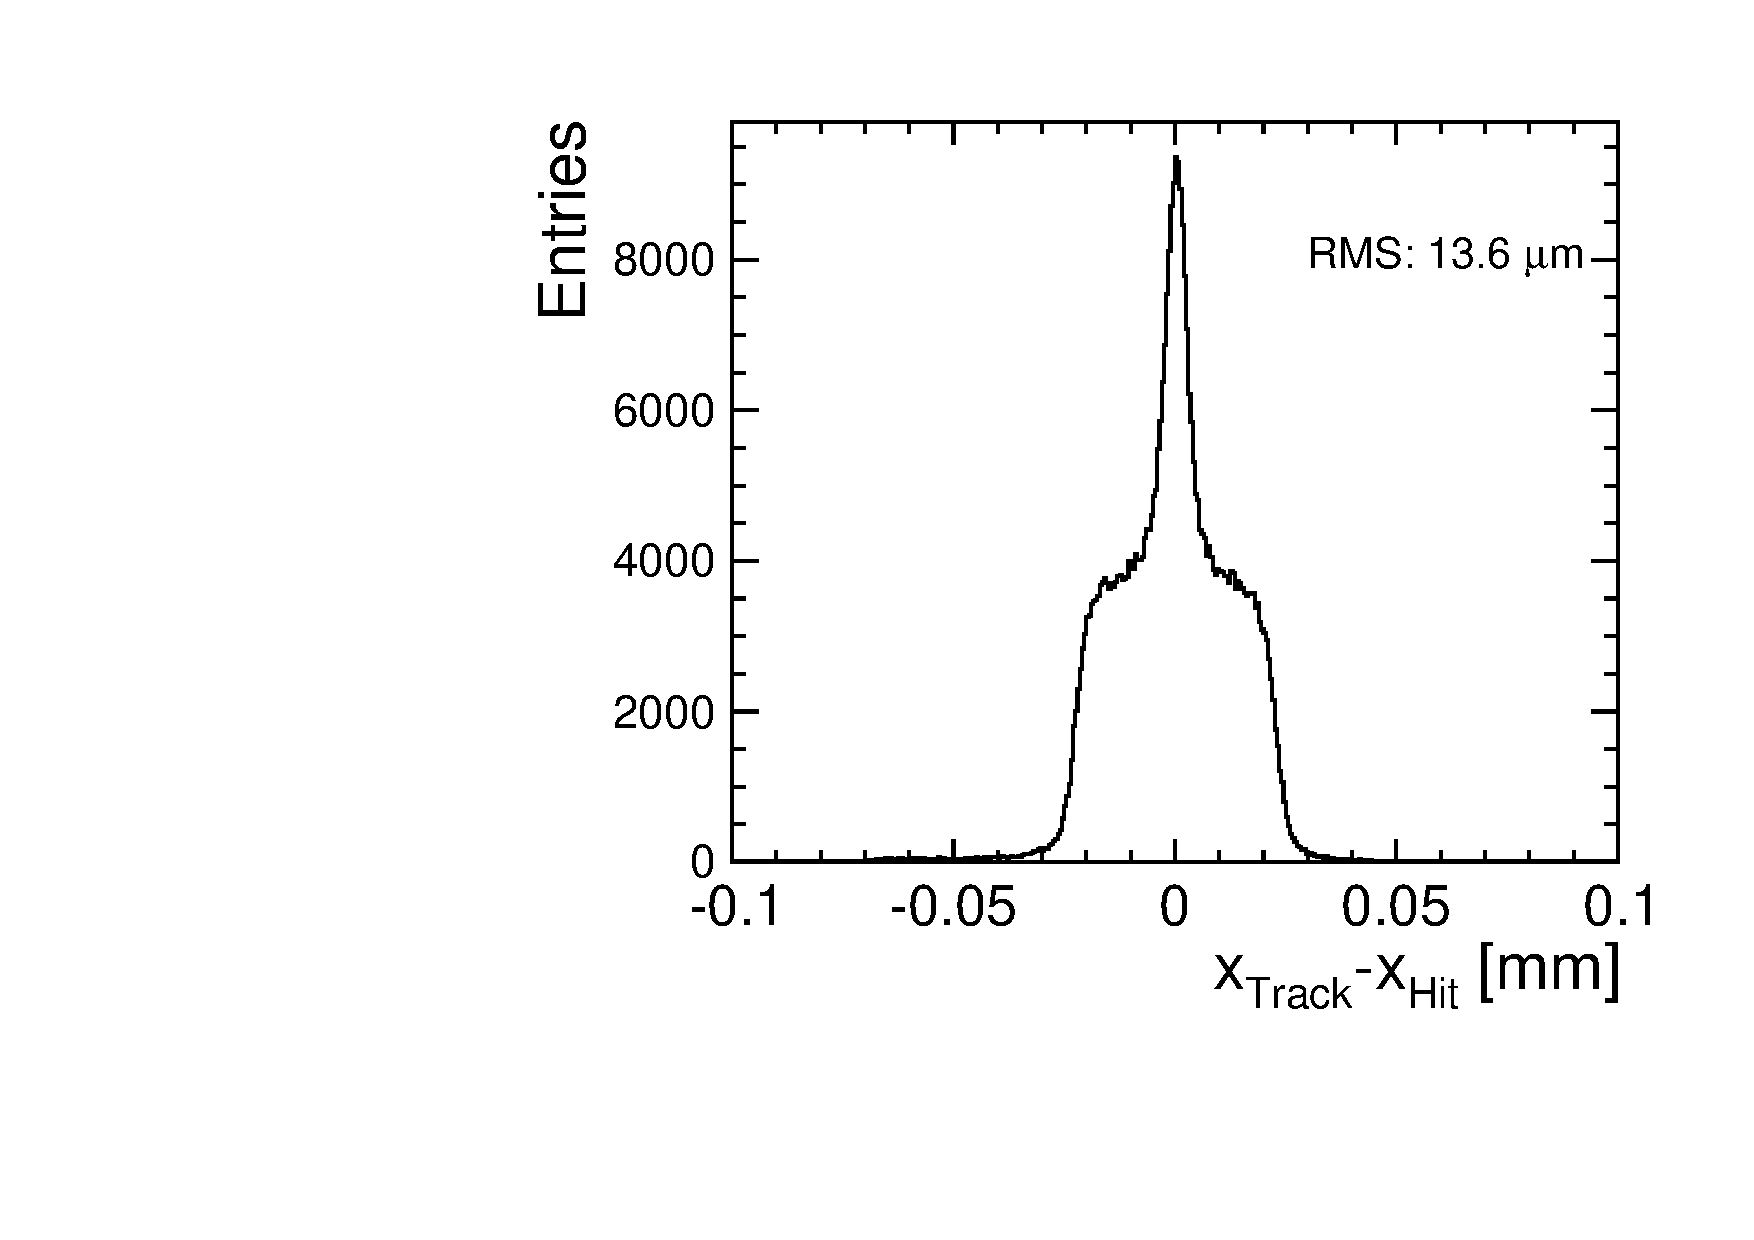
\includegraphics[width=\textwidth]{./figures/TestBeam/residualsHist_W5_E2.pdf}
%%     \caption{$100\,\micron$ sensor}
%%   \end{subfigure} \hfill
%%   \begin{subfigure}[b]{0.23\textwidth}
%%     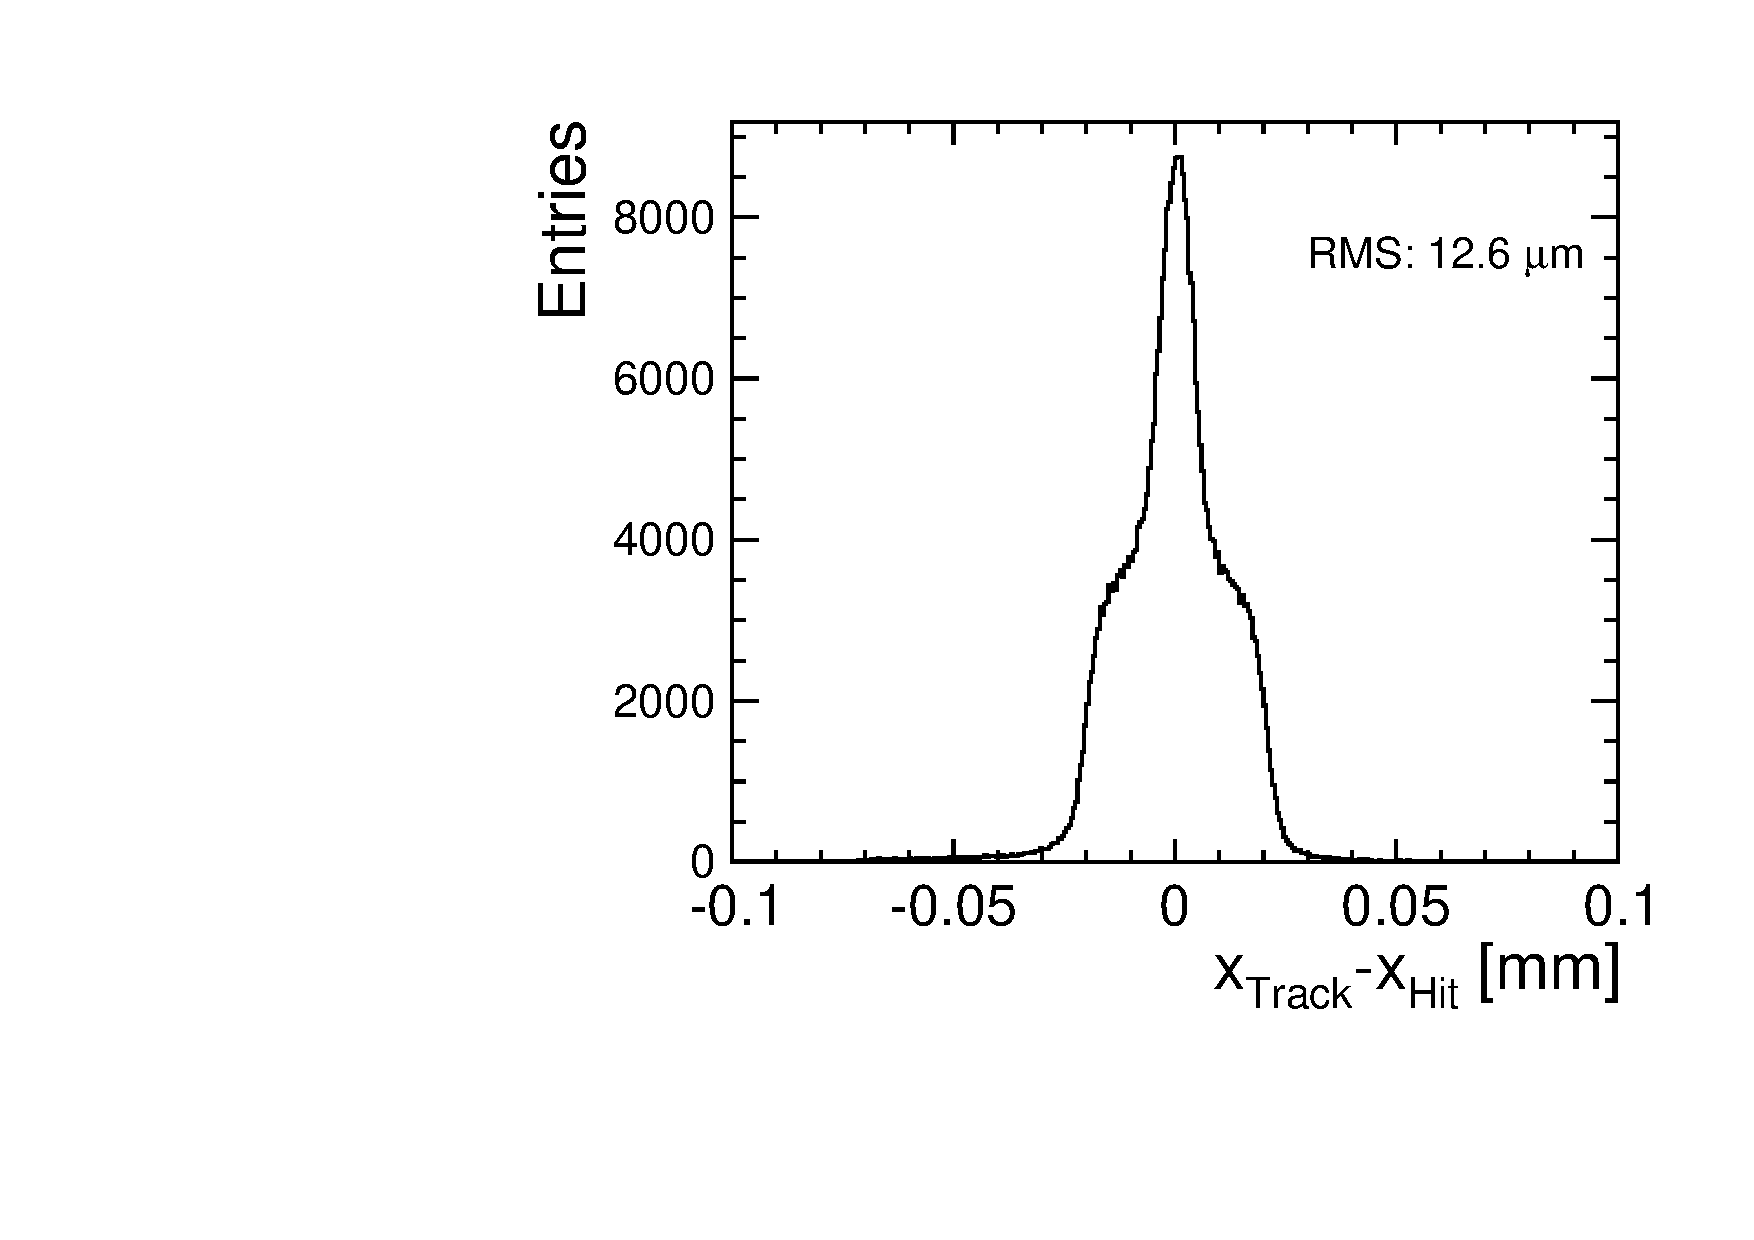
\includegraphics[width=\textwidth]{./figures/TestBeam/residualsHist_W5_F1.pdf}
%%     \caption{$150\,\micron$ sensor}
%%   \end{subfigure} \hfill
%%   \begin{subfigure}[b]{0.23\textwidth}

%%     \caption{$300\,\micron$ sensor}
%%   \end{subfigure}
%%   \caption{Examples of the residuals distributions in the x direction
%%     for the assemblies (a) W19\_C7, (b) W5\_E2 and (c) W5\_F1. The
%%     track resolution is not unfolded.}
%%   \label{fig:residualsHist_thickness}
%% \end{figure}


The factors affecting the fraction of different cluster sizes such as
the sensor thickness and the operating conditions of the assembly
(threshold and bias voltage) affect as well the
residuals. \cref{fig:Residuals_bias_threshold} shows the RMS of the
residuals in the x (column) and y (row) directions for a $50\,\micron$
thick sensor (assembly W19\_G7) as a function of the bias voltage and
the threshold. The residuals follow the same trend as the cluster size
distributions: higher fractions of single-pixel clusters result in
larger residuals.

% For other assemblies, these plots are shown in
% \cref{fig:Residuals_vs_biasVoltage,fig:Residuals_vs_Threshold}. 

\begin{figure}[htbp] \centering
  \begin{subfigure}[b]{0.45\textwidth}
    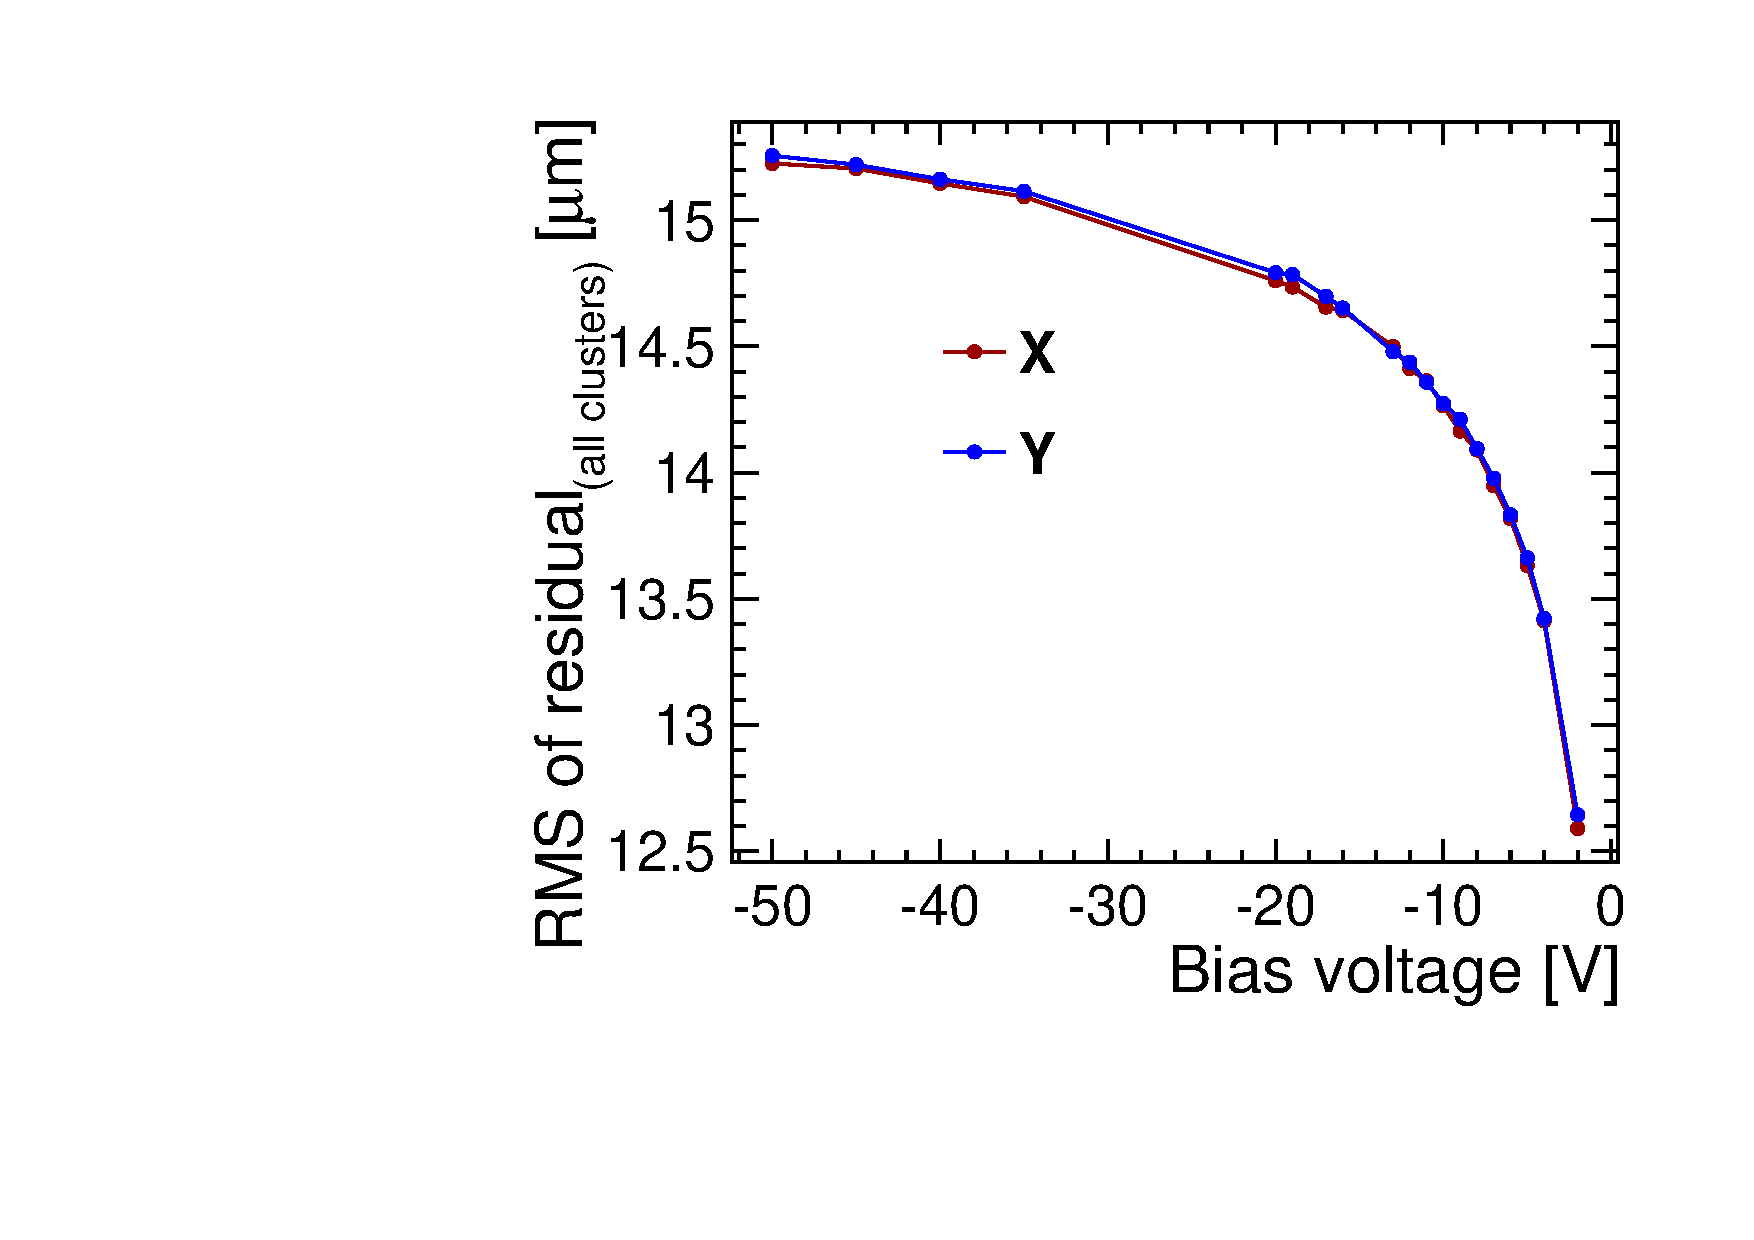
\includegraphics[width=\textwidth]{./figures/TestBeam/W19_G7_Residual_vs_bias.pdf}
    \caption{}
  \end{subfigure} \hfill
  \begin{subfigure}[b]{0.45\textwidth}
    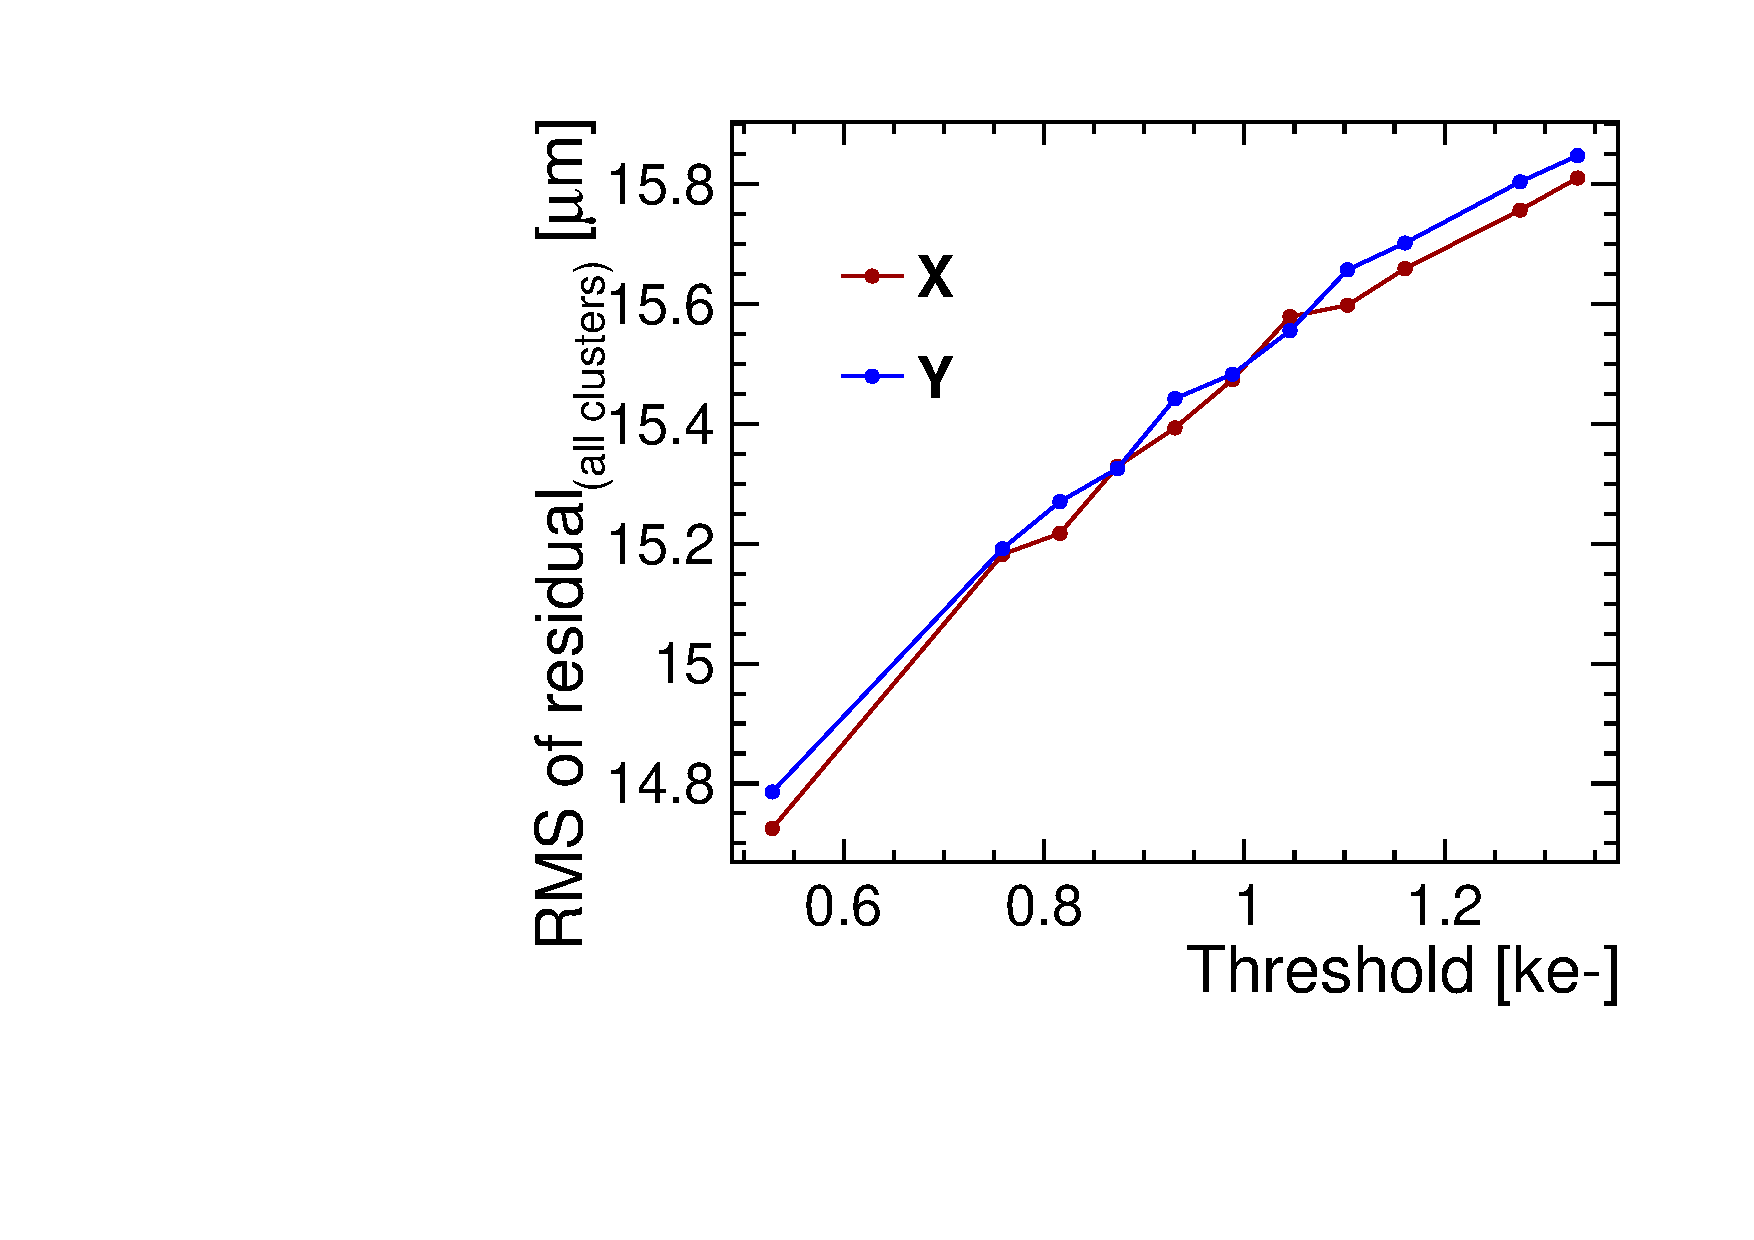
\includegraphics[width=\textwidth]{./figures/TestBeam/residuals_W0019_G07_THLscan.pdf}
    \caption{}
  \end{subfigure}
  \caption{The RMS of the residuals in x (column) and y (row)
    directions as a function of (a) bias voltage and (b) threshold for
    a $50\,\micron$ thick sensor (assembly W19\_G7).}
  \label{fig:Residuals_bias_threshold}
\end{figure}


For the assemblies operated at the nominal operating conditions, the
RMS of the residuals in the x and y directions as a function of the
sensor thickness are shown in \cref{fig:residuals_thickness}. For
thicker sensors the fraction of multi-pixel clusters is higher and
results in lower residuals. Again, a good agreement between data and
simulation is observed (less than $4\%$ deviation).

\begin{figure}[htbp] 
  \centering
  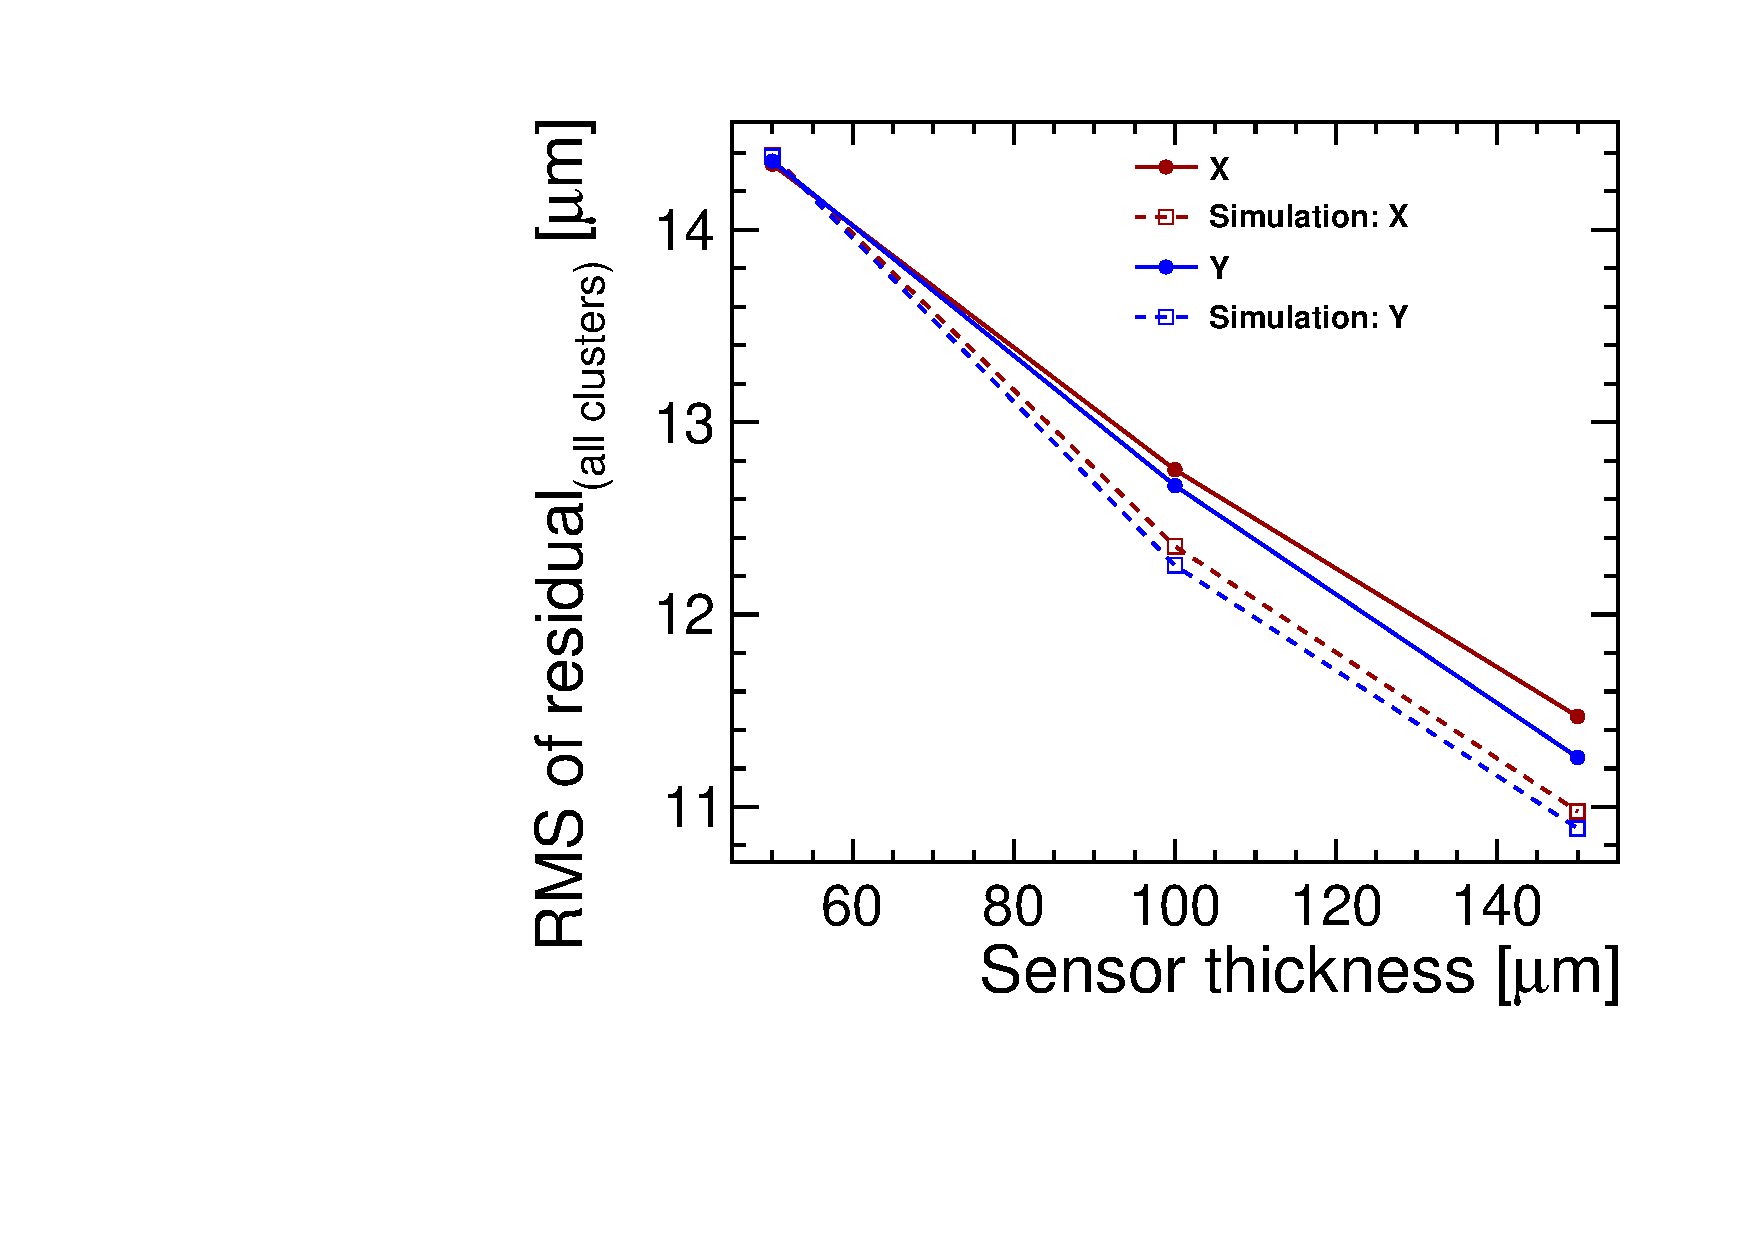
\includegraphics[width=0.5\textwidth]{./figures/TestBeam/residuals_vs_thickness.pdf}
  \caption{The RMS of the residuals in x and y directions as a
    function of the sensor thickness for assemblies operated at the
    nominal condition. The y-axis is zero-suppressed and the deviation
    between data and simulation is less than $4\%$.}
  \label{fig:residuals_thickness}
\end{figure}



%% --------------------------------------------- %%
\subsection{Detection efficiency}

The detection efficiency of the assemblies is defined as the fraction
of total number of hits matched to tracks (within a circle of radius
0.1~mm around the predicted track position) and the total number of
tracks projected to pass through the assembly. The efficiency is
calculated within the matrix of $256\times256$ pixels of the main
sensor area. The calculation of the efficiency does not exclude the
track hitting the masked or hot pixels, therefore the efficiency is
slightly lower than $100\%$ (see \cref{tab:numberOfMaskedPixels} for
the number of masked pixels during the data taking).

The detection efficiency is strongly related to the operating
threshold of the readout ASIC. With a lower threshold, smaller energy
depositions can be measured and it is more likely to detect a
particle. \cref{fig:efficiency_VS_Threshold} shows the detection
efficiency for different sensor thicknesses. For thinner sensors, the
energy deposition is lower and the efficiency drops more quickly by
increasing the threshold than for thick sensors.

\begin{figure}[htbp] 
  \centering
  \begin{subfigure}[b]{0.45\textwidth}
    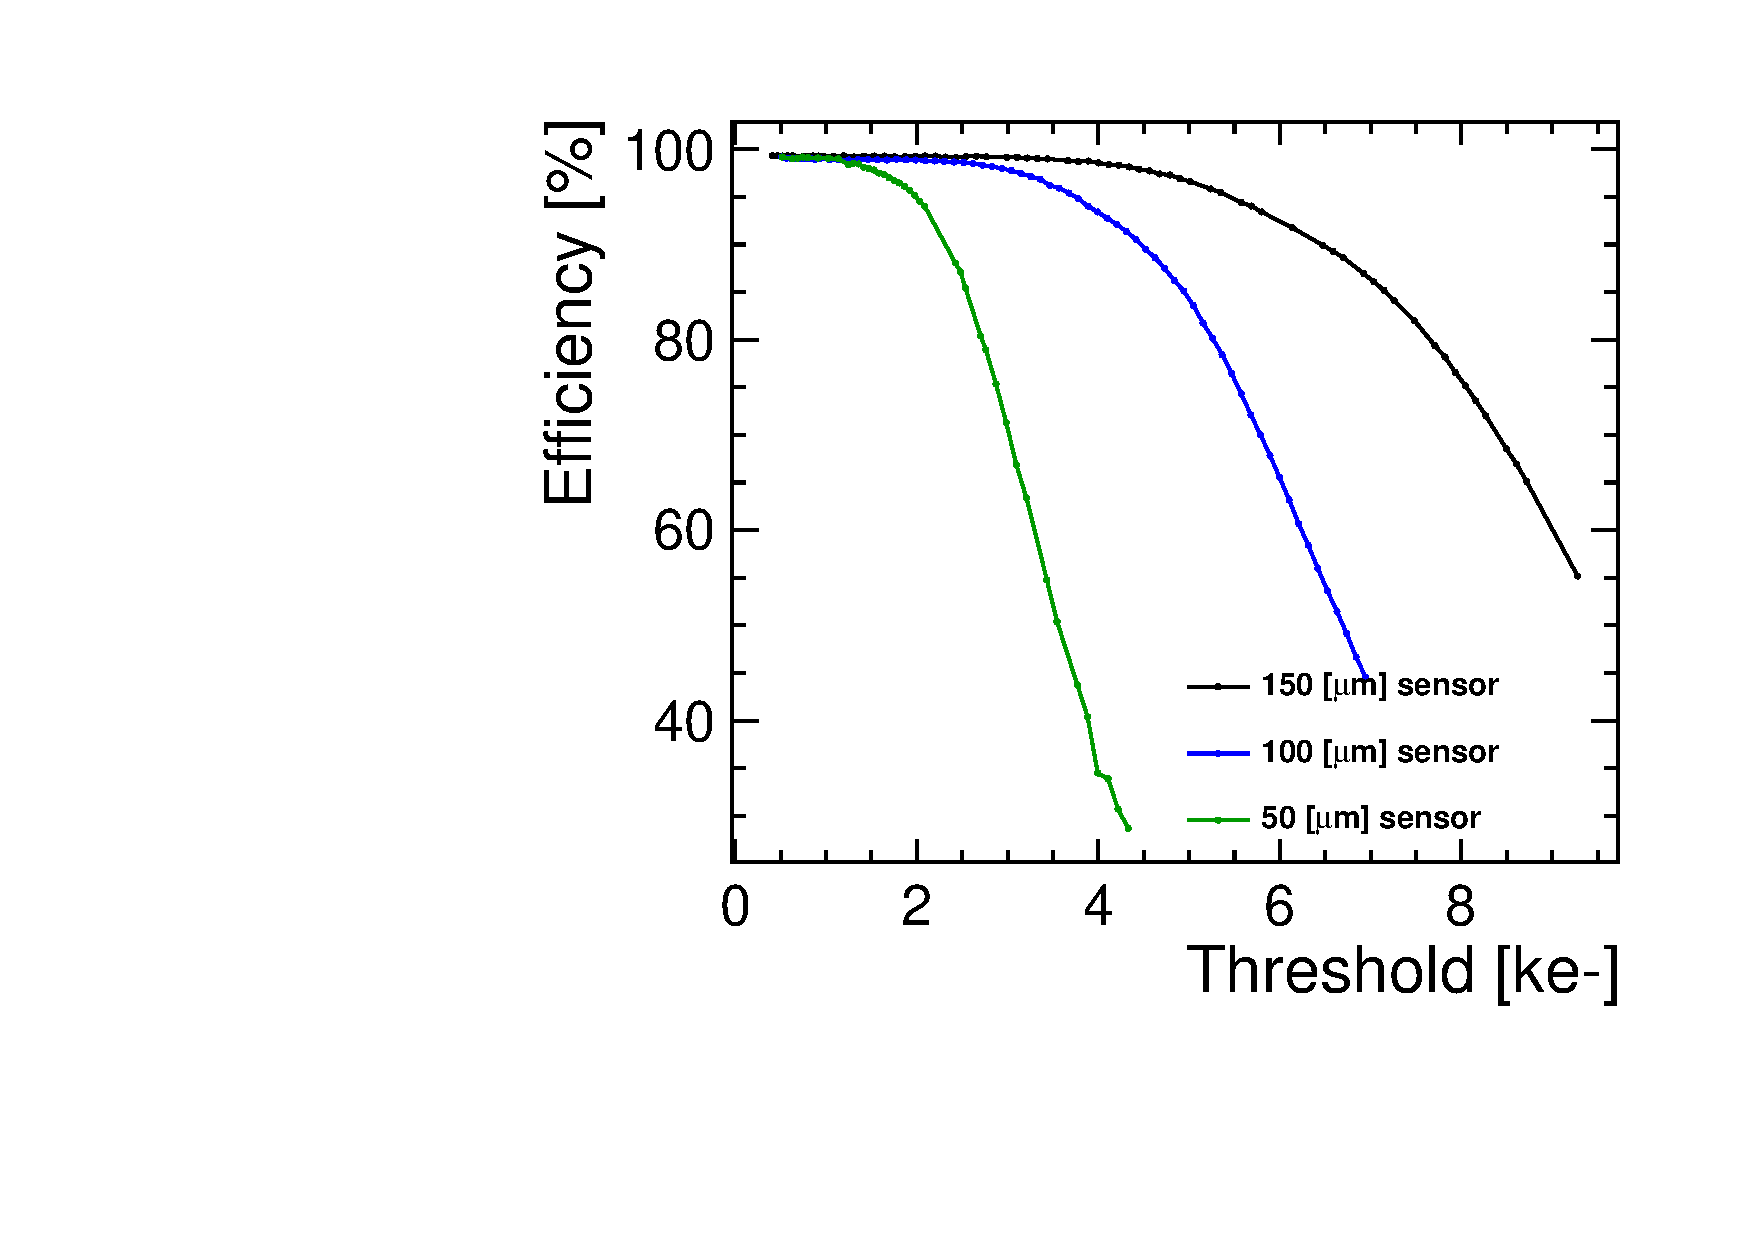
\includegraphics[width=\textwidth]{./figures/TestBeam/Efficiency_vs_THL.pdf}
    \caption{}
  \end{subfigure}\hfill
  \begin{subfigure}[b]{0.45\textwidth}
    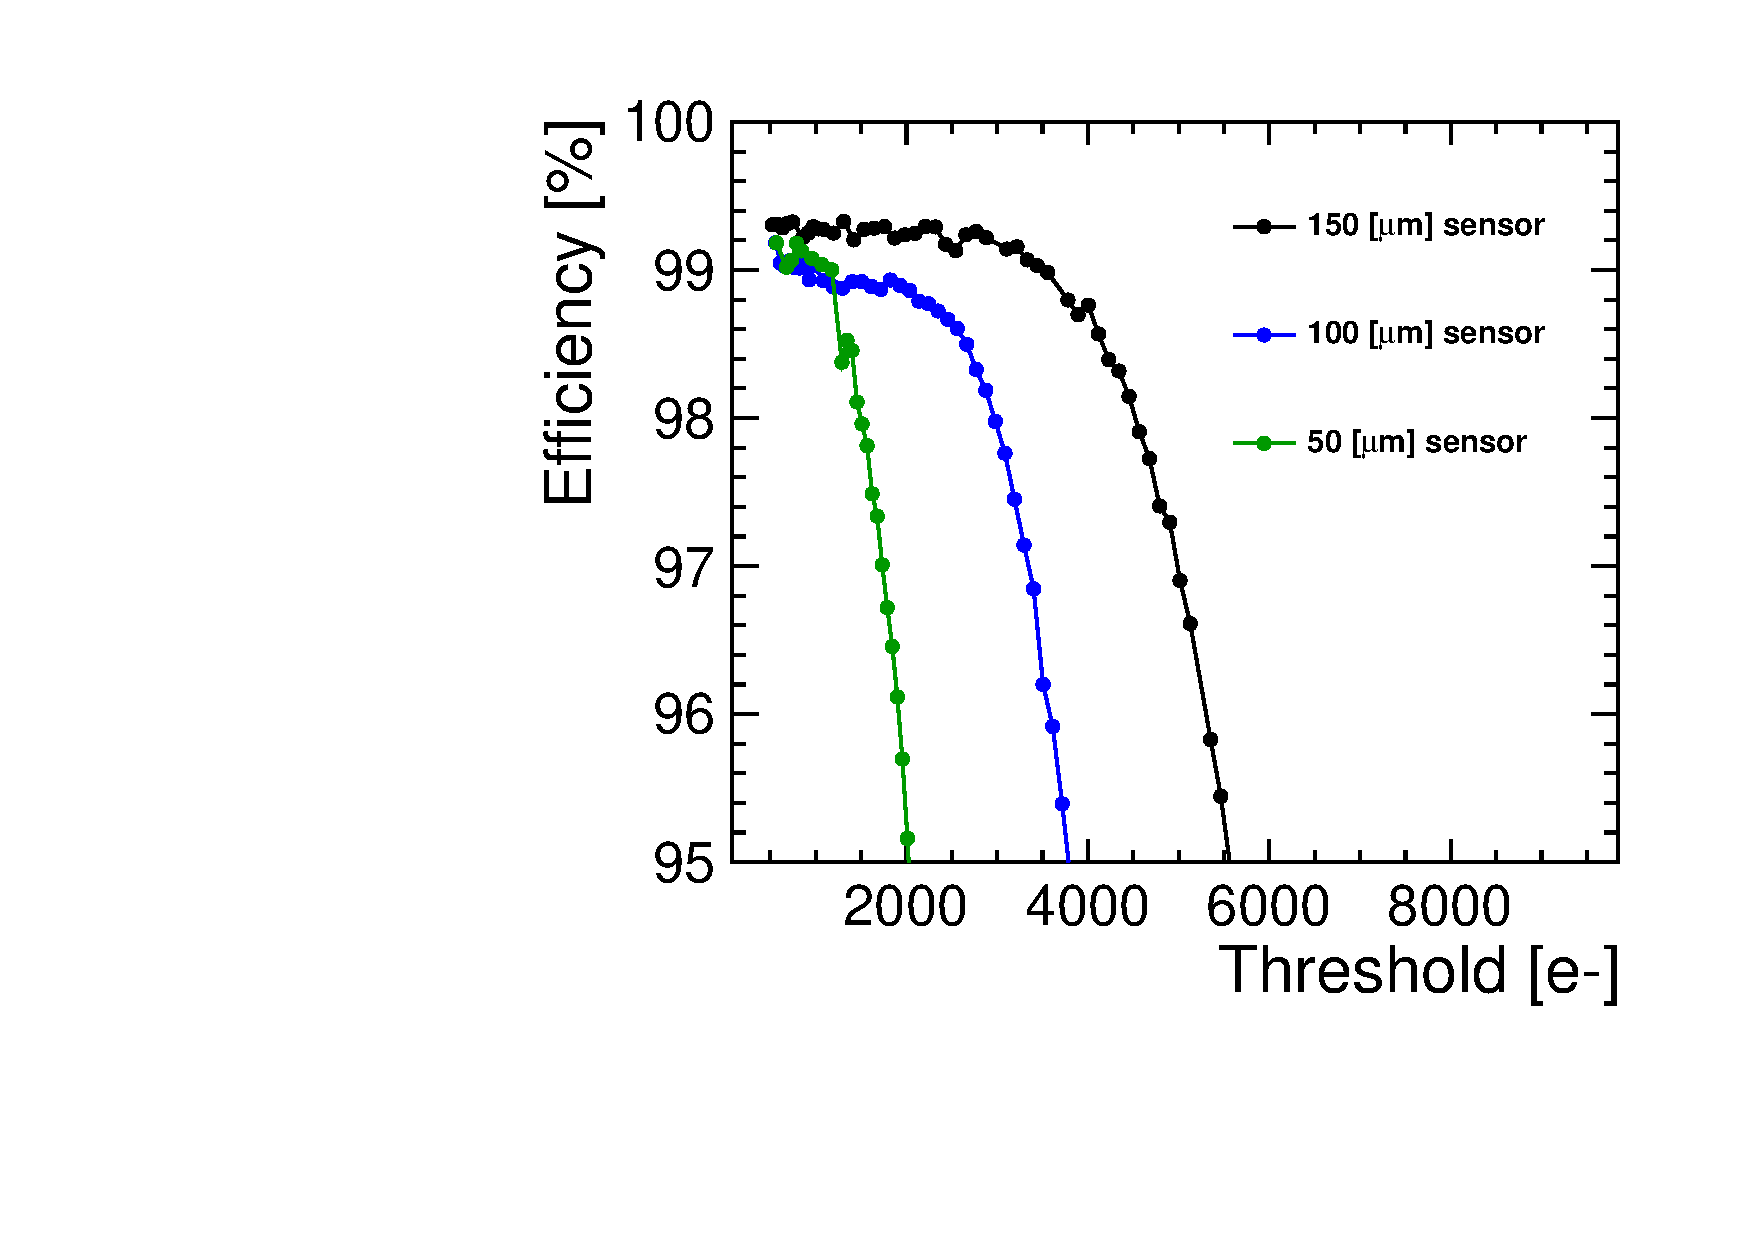
\includegraphics[width=\textwidth]{./figures/TestBeam/Efficiency_vs_THL_zoom.pdf}
    \caption{}
  \end{subfigure}
  \caption{(a) Global detection efficiency as a function of the
    threshold of the readout ASIC for different sensor thicknesses
    (for the assemblies W19\_L8, W5\_E2 and W5\_F1). (b) focuses on
    the efficiencies between $95\%$ and $100\%$.}
  \label{fig:efficiency_VS_Threshold}
\end{figure}

%% %% --------------------------------------------- %%
%% \section{Validation of the simulation}
%% \label{sec:ThinSensorSimuValidation}

%% The assemblies are simulated at the nominal operating conditions. The
%% cluster size, the residuals and the energy deposition distributions
%% are shown in
%% \cref{fig:G4_simu_data_cluSize,fig:G4_simu_data_Residuals,fig:G4_simu_data_Edep}
%% comparing data and simulations. The track resolution of
%% $\sim2\,\micron$ is not unfolded in the residuals distribution. The
%% simulation is in good agreement with the data and is used to predict
%% the performance of smaller pixel pitches.

%% --------------------------------------------- %%
\section{Extrapolation to smaller pixels}

The Timepix3 readout ASIC has been used as a test vehicle for the
characterisation of thin sensors. The test-beam measurements and the
AllPix simulations show a good agreement. However, the Timepix3 ASIC
has a pixel pitch of $55\,\micron$ and the goal for the CLIC vertex
detector is to achieve pixels of pitch $25\,\micron$. The CLICpix
readout ASIC~\cite{clicpix} implemented in 65~nm CMOS technology with
a pitch of $25\,\micron$ is under development. A single-chip indium
bump bonding process for $25\,\micron$ pitch is under development at
SLAC~\cite{SLACBumpBonding} and a few assemblies with $50\,\micron$
and $200\,\micron$ thick planar sensors are successfully bump-bonded
to CLICpix ASICs. These assemblies are currently under
study~\cite{AlipourTehrani2016}.

Previously, we have seen a good agreement between the AllPix
simulations and the data taken in the test beams for thin silicon
sensors. The simulation can be used to predict the performance of thin
sensors and small pitches in terms of charge sharing.

Figure~\ref{fig:cluSize25Pitch} shows the cluster-size distribution
and the hit residuals (comparing the hit and the MC truth positions)
for an extrapolation of the simulation to small pixels of size
$10\,\micron$ to $55\,\micron$ with $50\,\micron$ thick sensors with a
Timepix3-type readout ASIC operated at 500 electrons threshold with
10-bit TOT measurement and an electronic noise of $\sim80$
electrons. The same digitiser as the one used to validate the
simulation is used for the extrapolation. Even with a small pitch of
$25\,\micron$ as foreseen for the CLIC vertex detector, in such thin
sensors, $\sim~70\%$ of clusters originating from minimum ionising
particles contain one pixel (the fraction of single-pixel clusters
with a $55\,\micron$ pitch is $\sim~83\%$). The residual distribution
is therefore dominated by the broad peak from single-pixel clusters
and the resulting resolution of $\sim~6\,\micron$ is still
significantly worse than the required $3\,\micron$. Based on
simulations, it can be concluded that the required resolution can not
be achieved with planar sensors of $50\,\micron$ thickness and
$25\,\micron$ pitch. A pixel pitch of $10\,\micron$ allows for
achieving a resolution of $\sim~3\,\micron$ as required by CLIC. New
sensor concepts with enhanced charge sharing~\cite{Jansen2016242} or
integrated technologies with even smaller pixel
pitch~\cite{Arai:2011ara} are therefore required.


% the $25\,\micron$ pitch. Smaller pixels can show
% other limiting factors. The CLIC pixel detector R\&D is considering
% new solution where planar sensors are not used.

\begin{figure}[htbp]\centering
  \begin{subfigure}[b]{0.45\textwidth}
    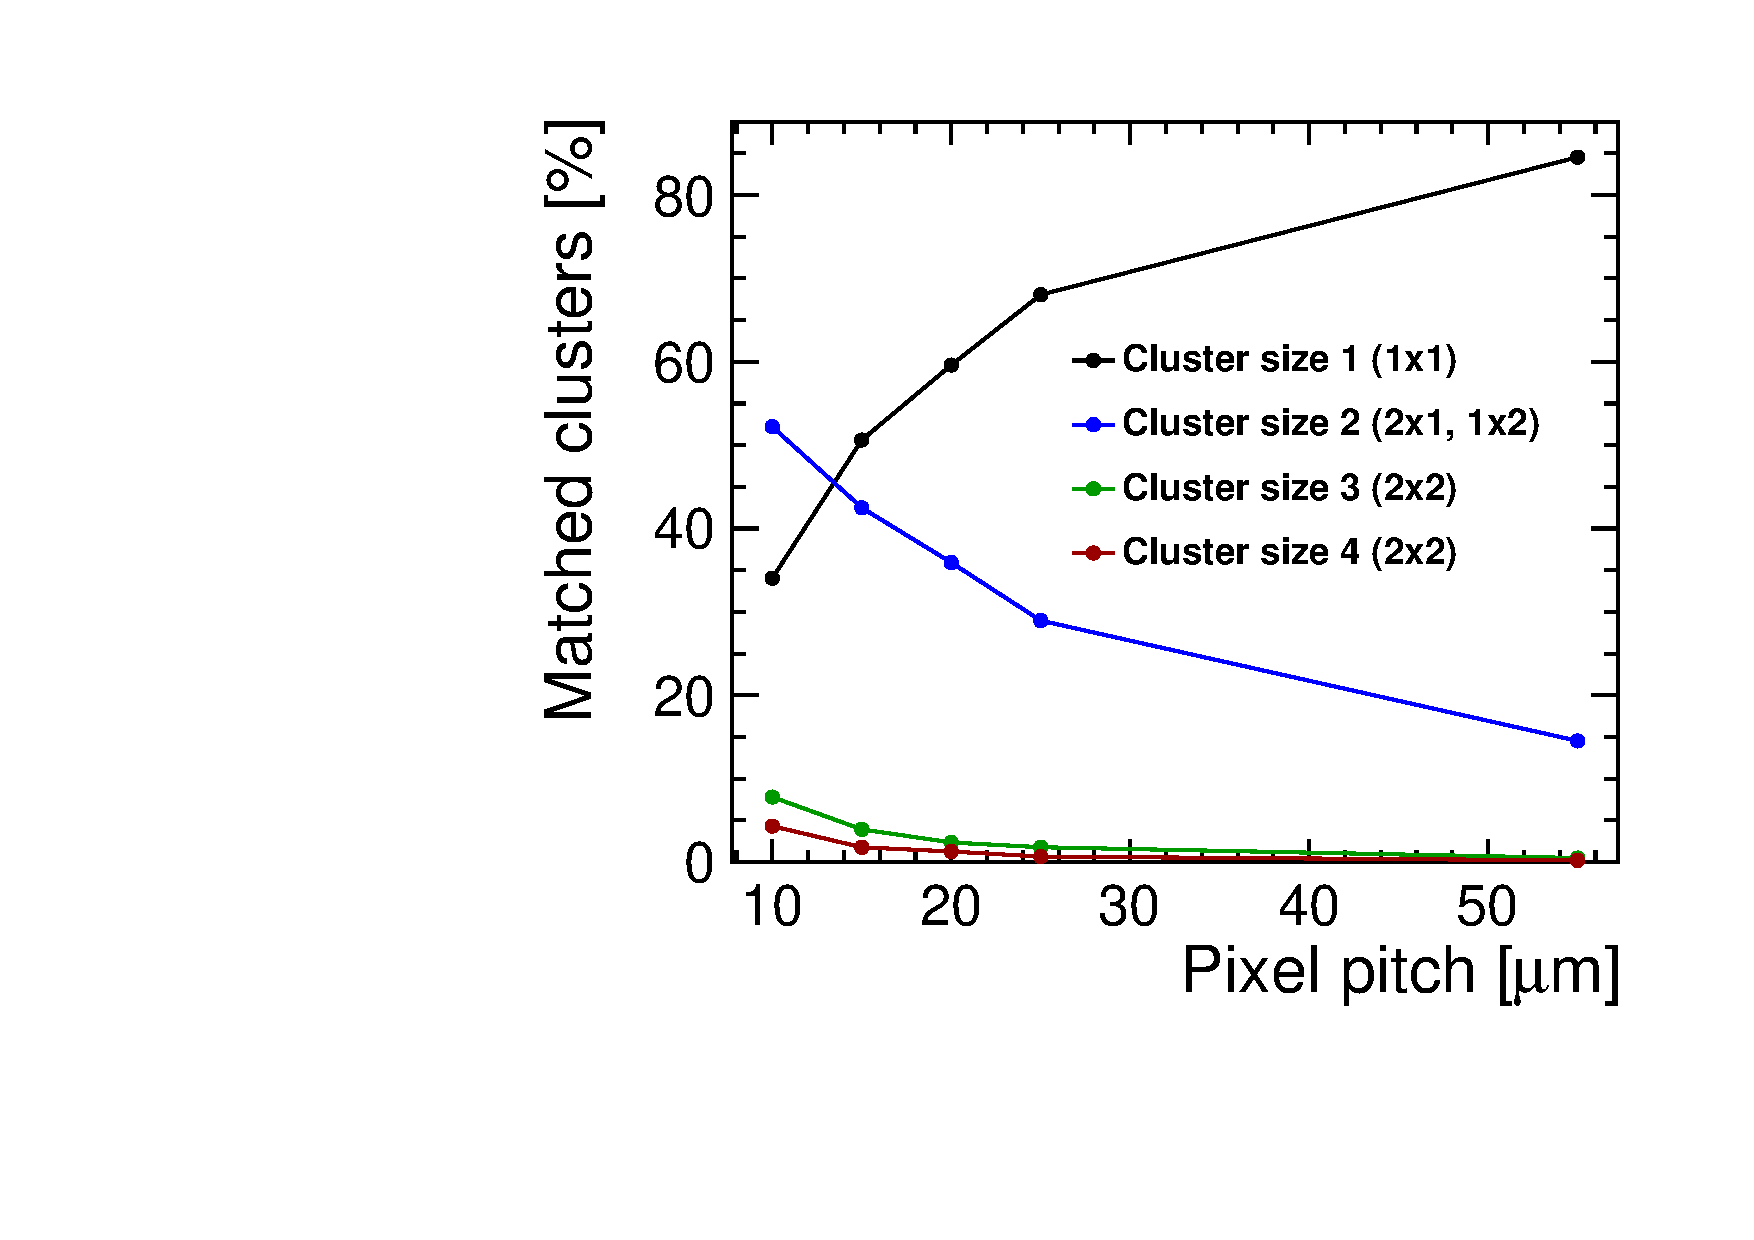
\includegraphics[width=\textwidth]{figures/TestBeam/ClusterSize_extrapolationSmallerPixels.pdf}
    \caption{}
  \end{subfigure}\hfill
  \begin{subfigure}[b]{0.45\textwidth}
    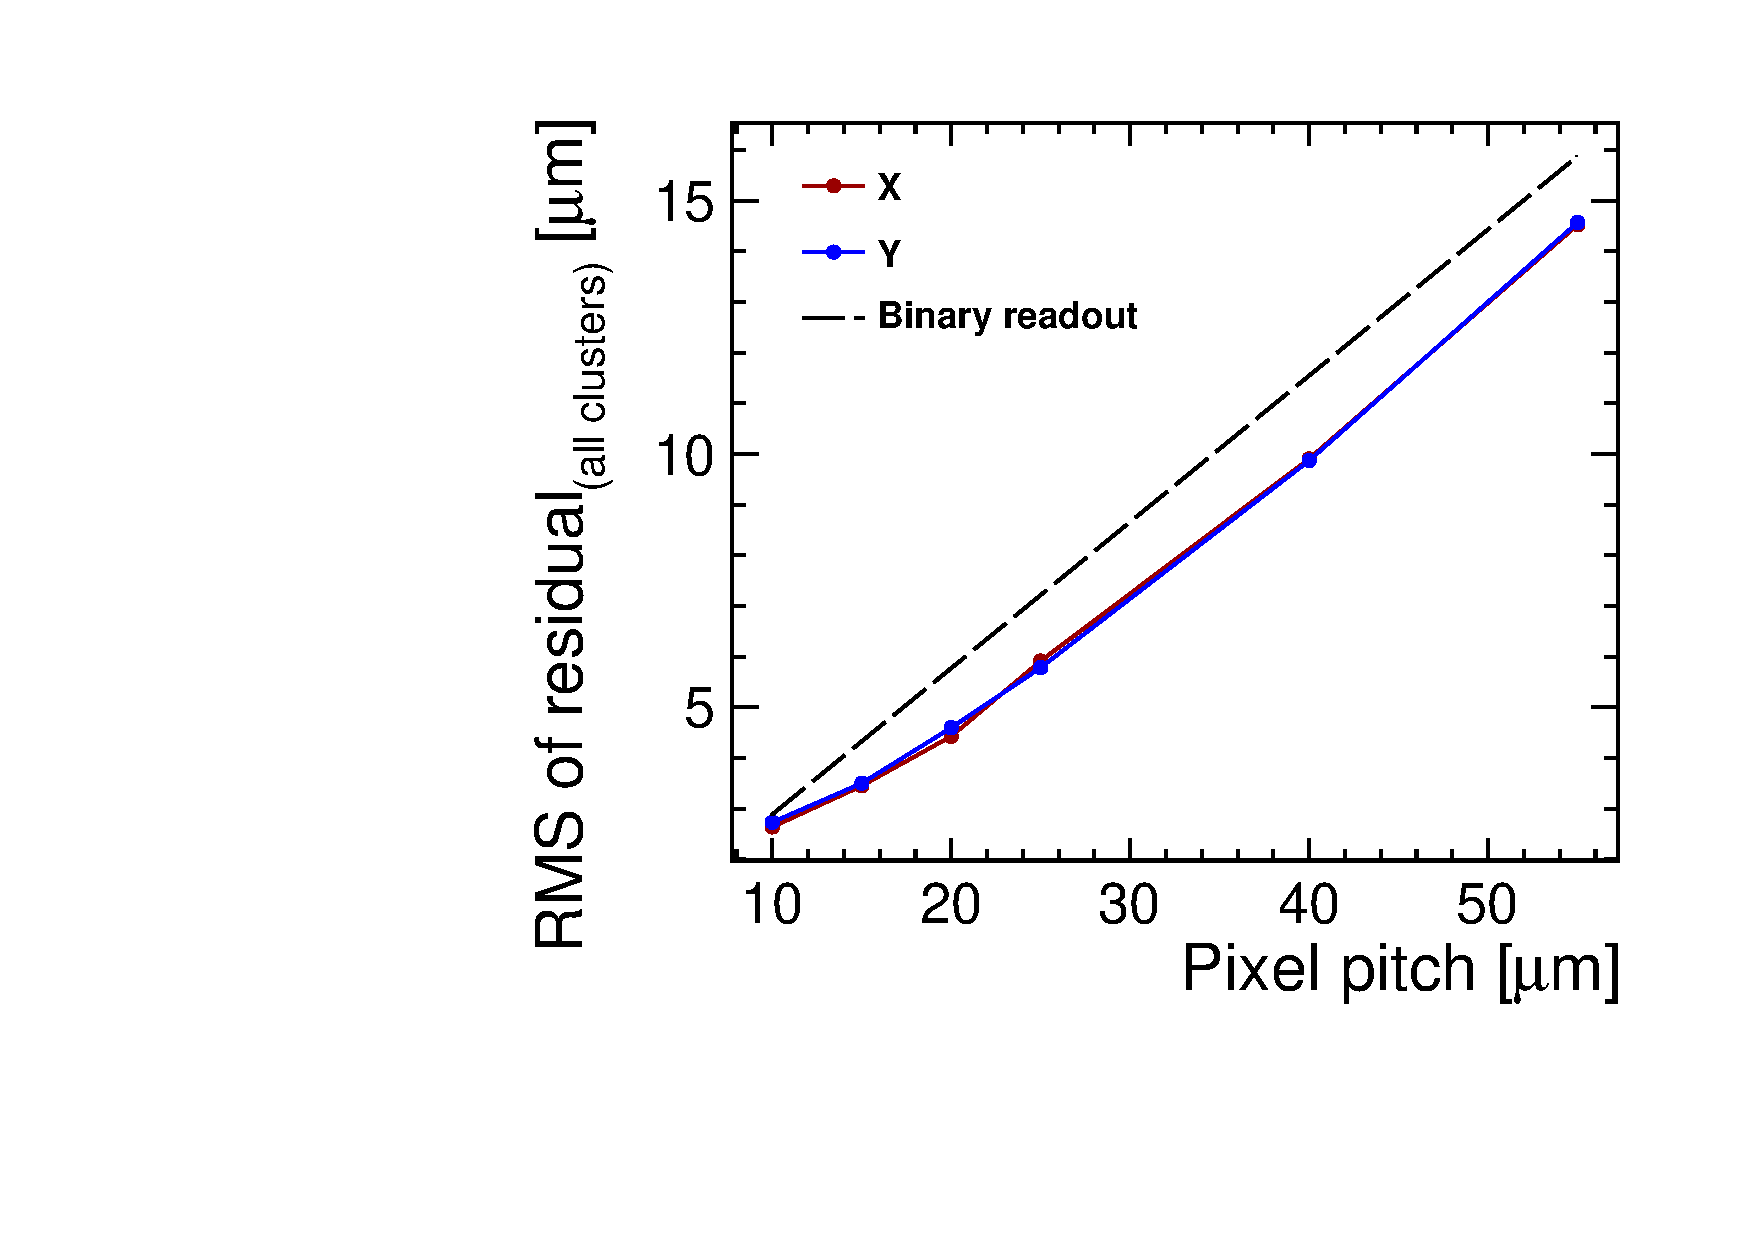
\includegraphics[width=\textwidth]{figures/TestBeam/RMS_extrapolationSmallerPixels.pdf}
    \caption{}
  \end{subfigure}
  \caption{(a) Cluster-size distribution and (b) hit residuals,
    comparing the hit and the MC truth position, for the extrapolation
    of the simulation to small pixel sizes with a $50\,\micron$ thick
    sensor and a threshold of $\sim~500$ electrons. Binary readout
    refers to the geometric resolution of pitch/$\sqrt{12}$.}
  \label{fig:cluSize25Pitch}
\end{figure}



%% \begin{figure}[htbp]\centering
%%   \begin{subfigure}[b]{0.45\textwidth}
%%     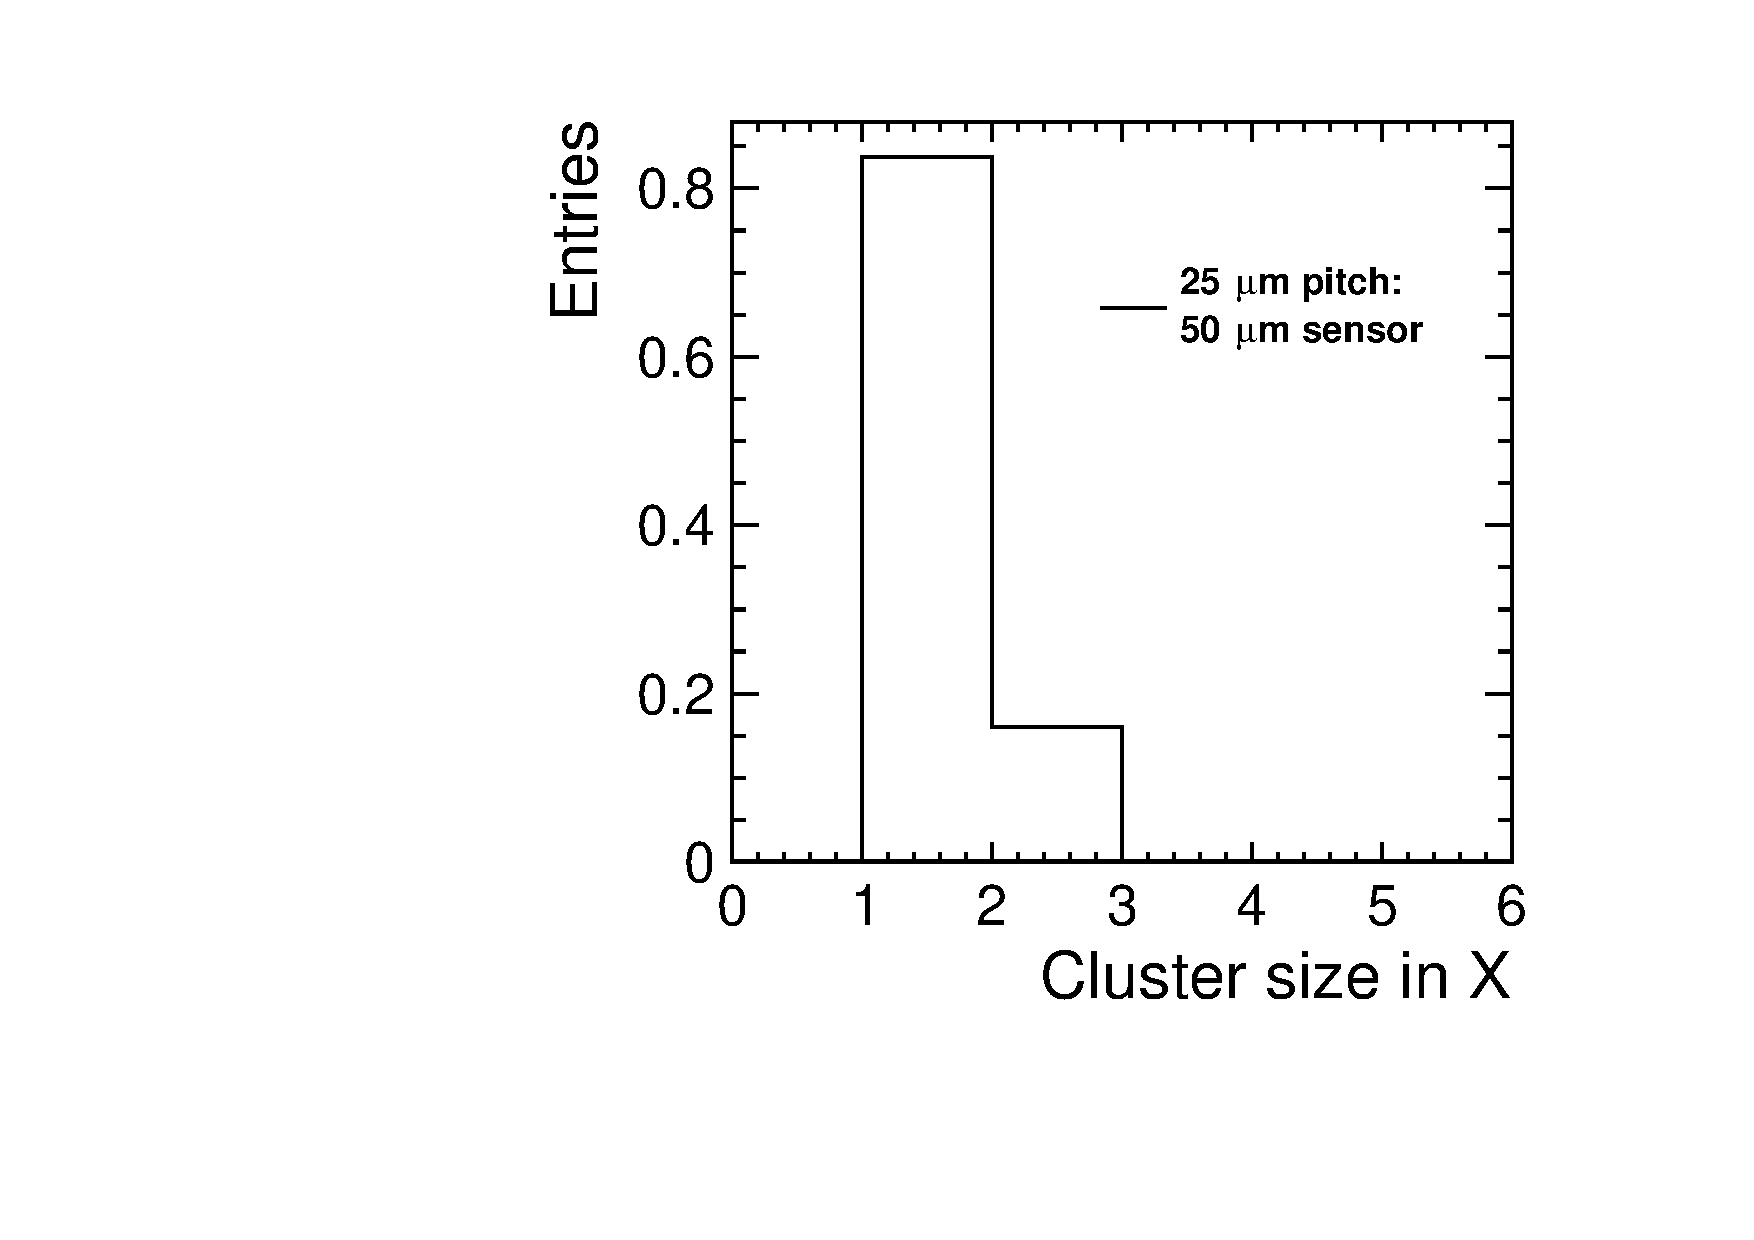
\includegraphics[width=\textwidth]{figures/TestBeam/ClusterSize_TPX3_CLICpix.pdf}
%%     \caption{}
%%   \end{subfigure}\hfill
%%   \begin{subfigure}[b]{0.45\textwidth}
%%     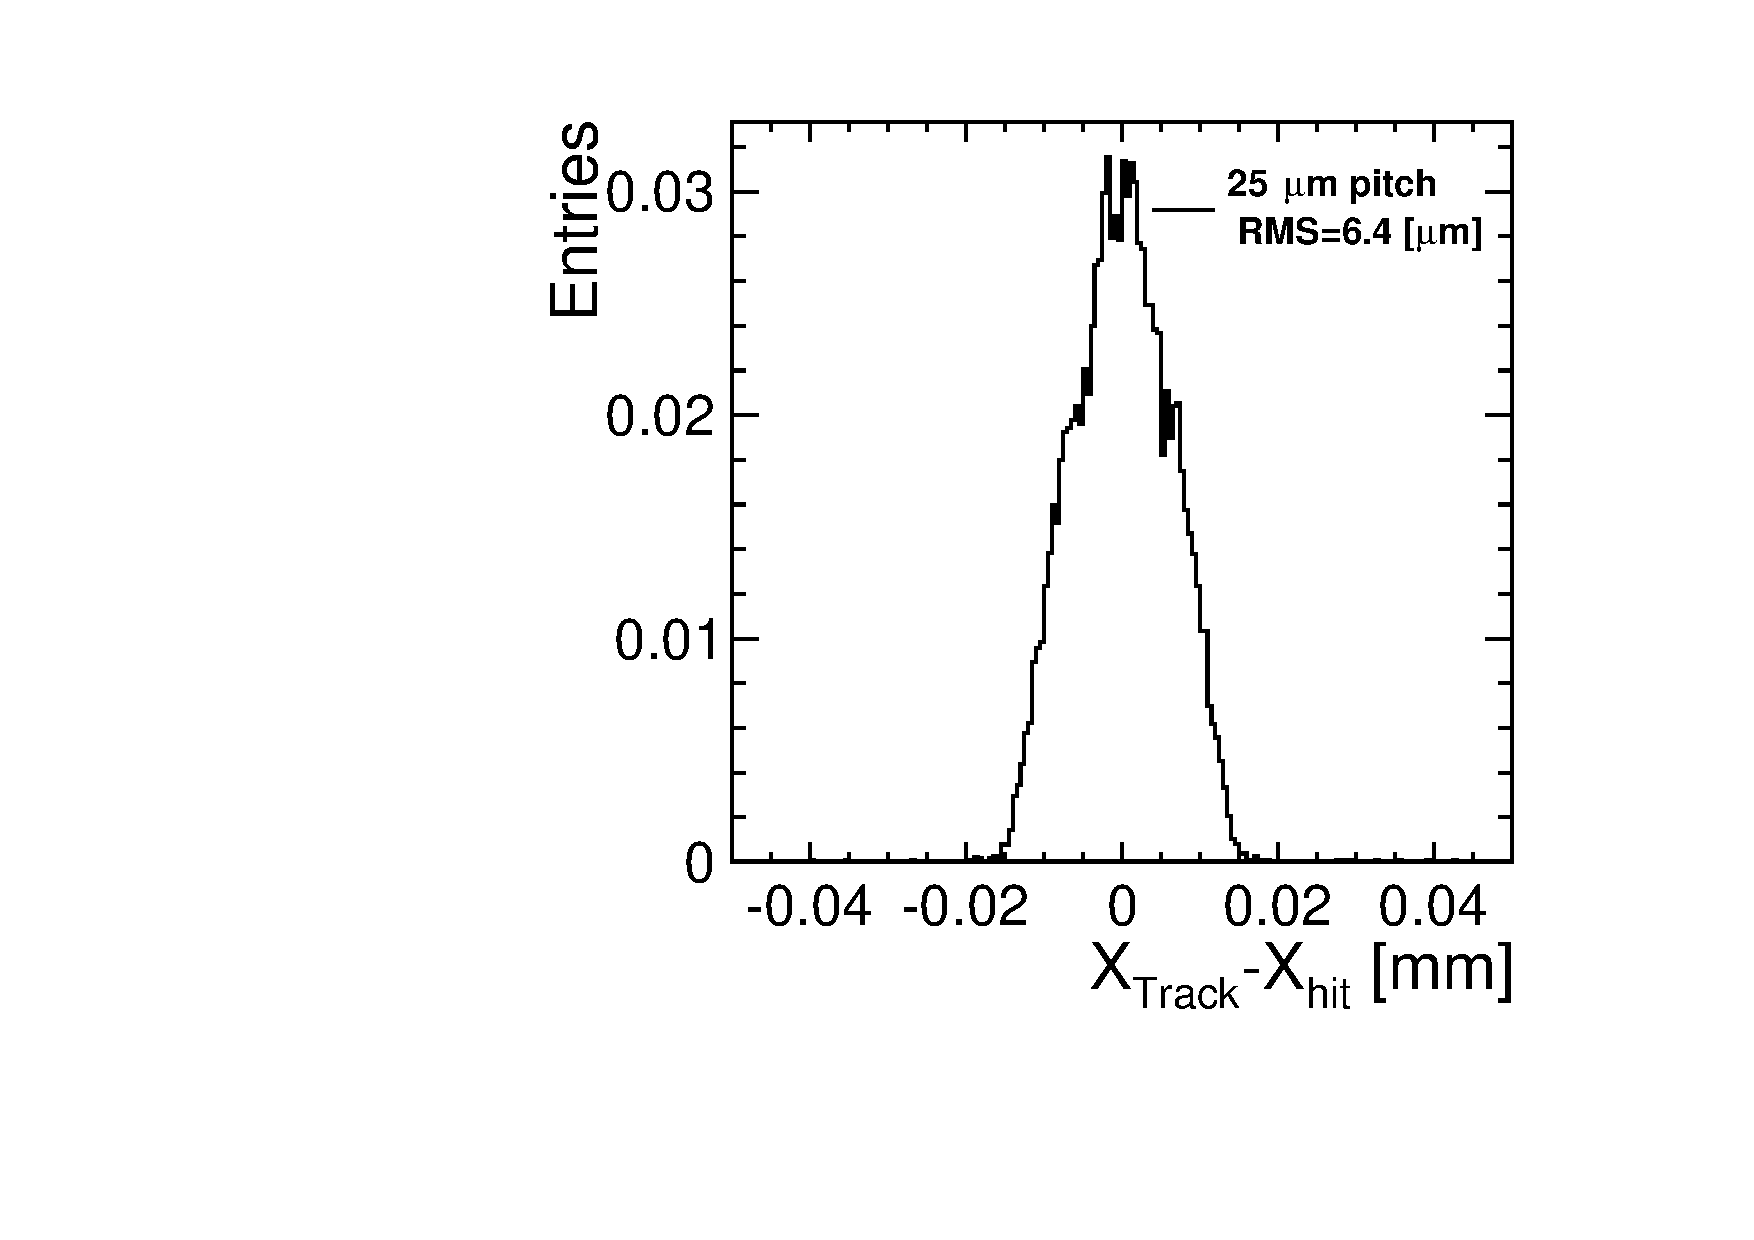
\includegraphics[width=\textwidth]{figures/TestBeam/ResolutionX_TPX3_CLICpix.pdf}
%%     \caption{}
%%   \end{subfigure}
%%   \caption{(a) Cluster-size distribution and (b) hit residuals in
%%     x-direction for the extrapolation of the simulation to
%%     $25\,\micron$ pixel pitch with a $50\,\micron$ thick sensor and a
%%     threshold of $\sim$500 electrons.}
%%   \label{fig:cluSize25Pitch}
%% \end{figure}





\section{Summary}
\label{sec:Summary_ThinSensors}

Test-beam measurements and \textsc{Geant4}-based simulation studies
for thin sensors using the Timepix3 ASIC are in good agreement. The
simplified model for the diffusion of charges in silicon as described
in \cref{sec:allpix_digitisation} gives a good agreement with data in
terms of energy-deposition spectrum, cluster-size distribution and
residuals distribution. Therefore, the simulation is used for
predicting the resolution of $50\,\micron$ thin sensors with small
pixel sizes of $25\,\micron$. This prediction shows the difficulty to
achieve the required 3 um resolution with very thin planar sensors.


%% \begin{figure}[htbp] 
%%   \centering
%%   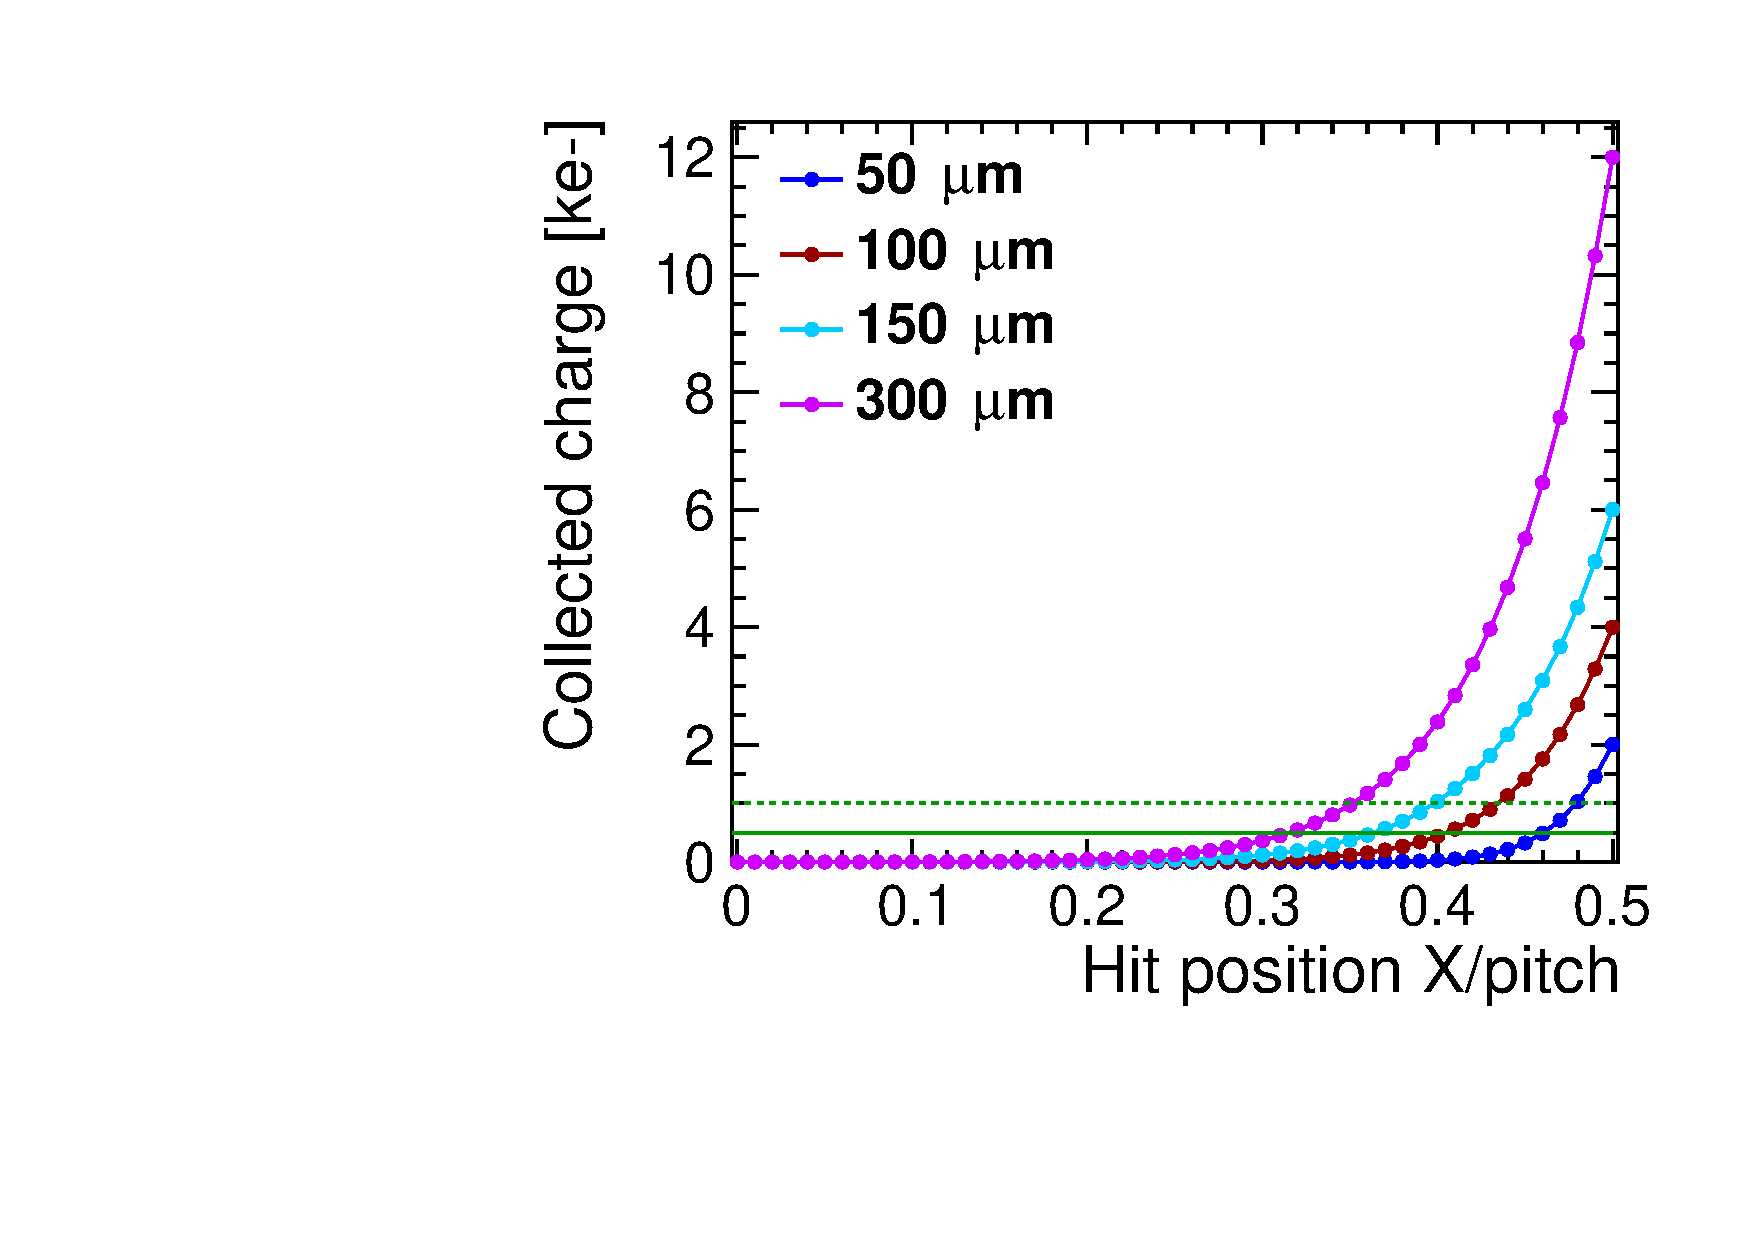
\includegraphics[width=0.5\textwidth]{./figures/TestBeam/chargeSharing_theory.pdf}
%%   \caption{Thresholds at 500 at 1000 electrons are shown in green lines.}
%%   \label{fig:chargeSharing_theory}
%% \end{figure}

%% %% --------------------------------------------- %%
%% \begin{figure}[htbp] \centering
%%   \begin{subfigure}[b]{0.45\textwidth}
%%     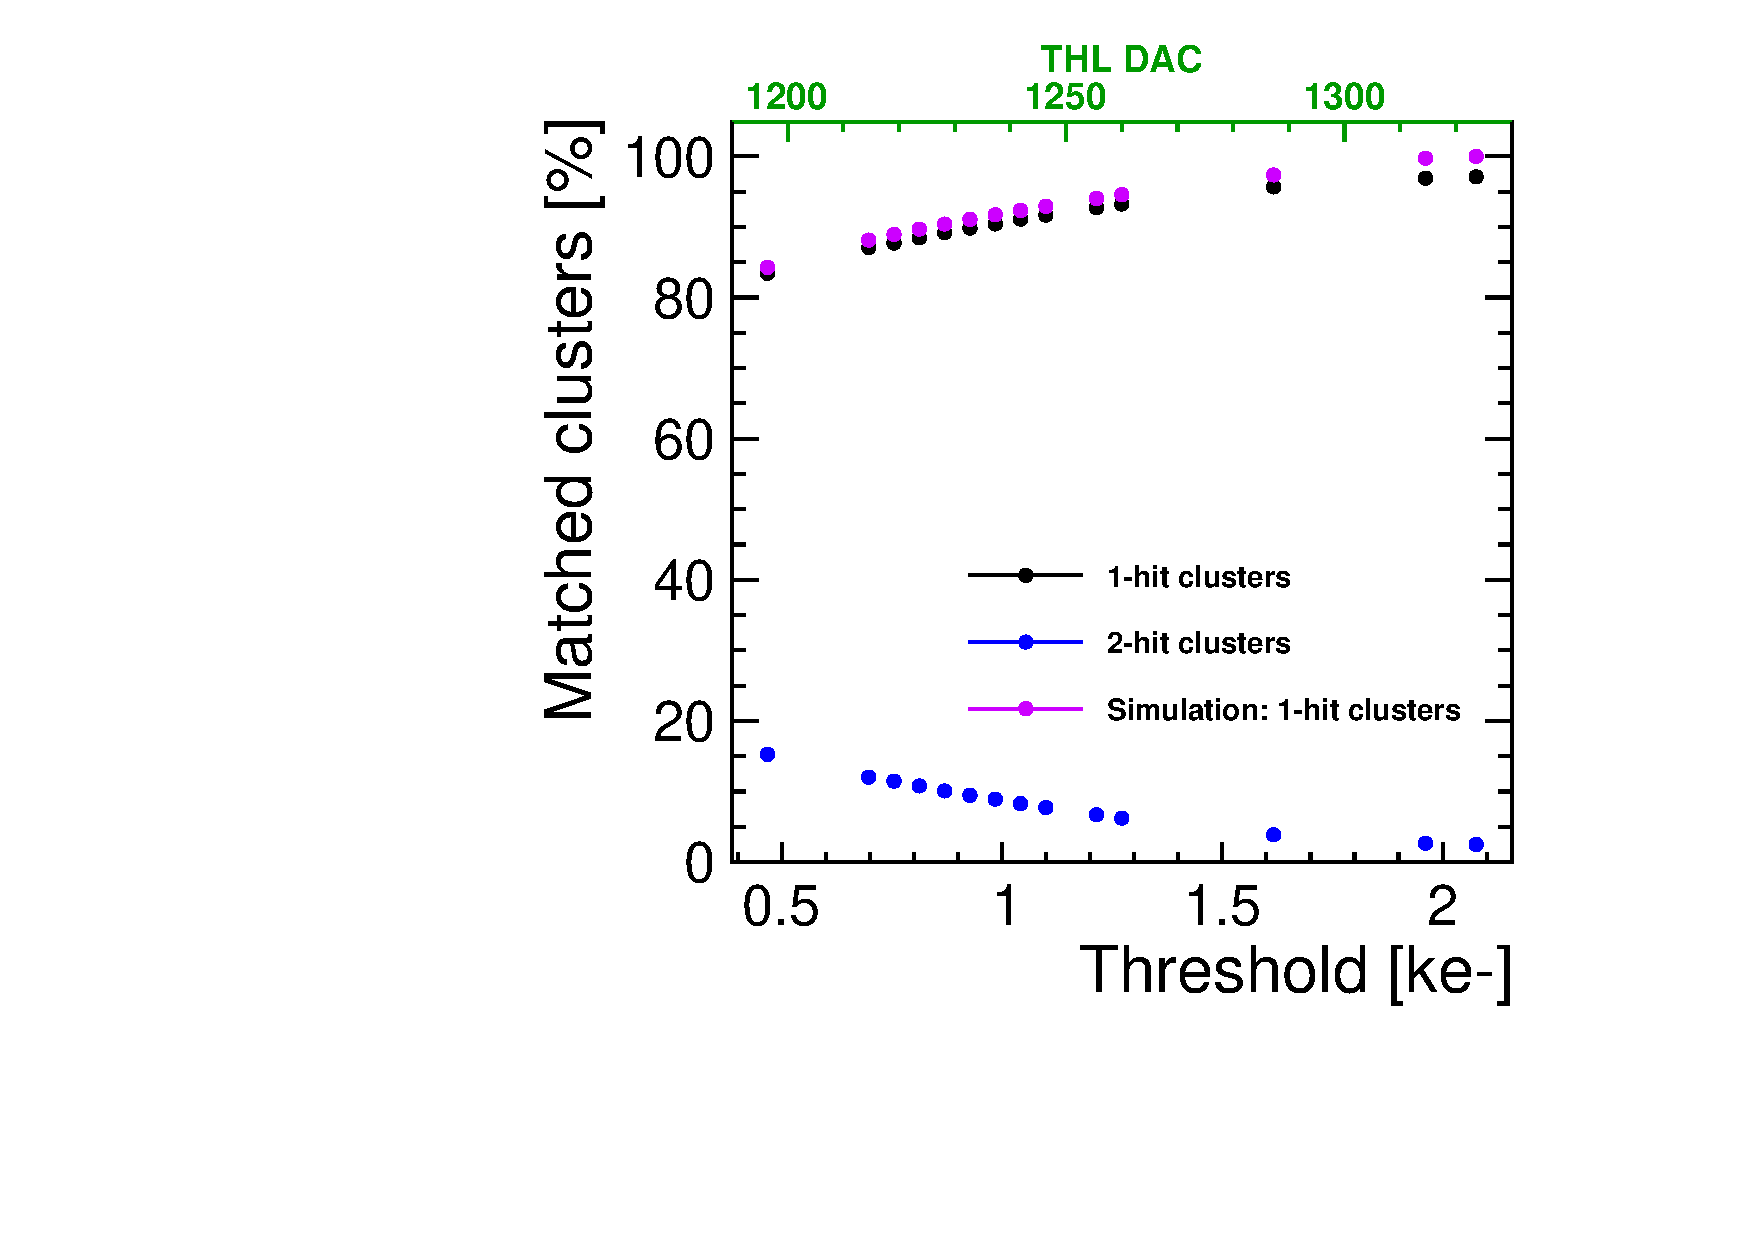
\includegraphics[width=\textwidth]{./figures/TestBeam/ThresholdScan_W0019_G07.pdf}
%%     \caption{}
%%   \end{subfigure} \hfill
%%   \begin{subfigure}[b]{0.45\textwidth}
%%     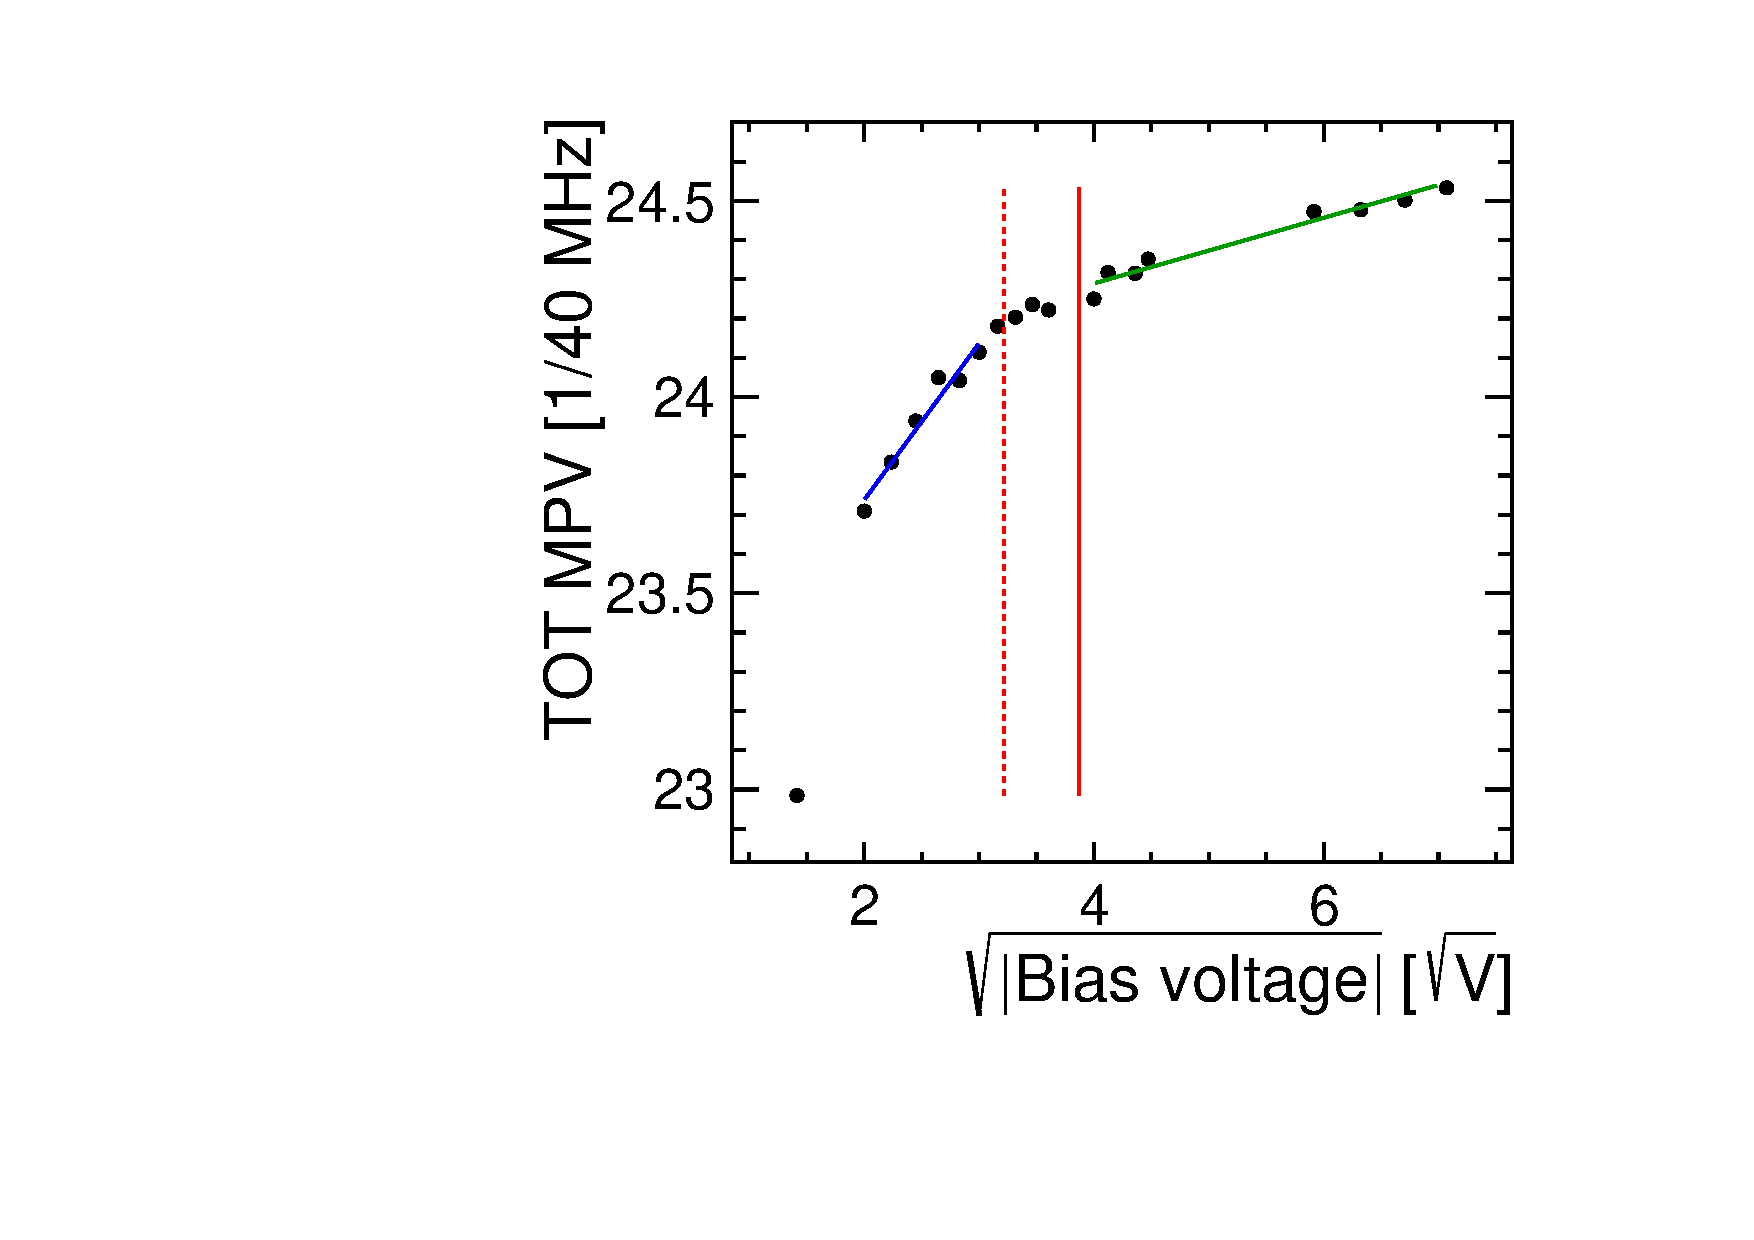
\includegraphics[width=\textwidth]{./figures/TestBeam/depletionVoltage_W0019_G07.pdf}
%%     \caption{}
%%   \end{subfigure}
%%   \caption{20-NGR (W19\_G7): bias and voltage scan.}
%%   \label{fig:Timepix3_THLscan_Vdep_G7}
%% \end{figure}

%% \begin{figure}[htbp] \centering
%%   \begin{subfigure}[b]{0.45\textwidth}
%%     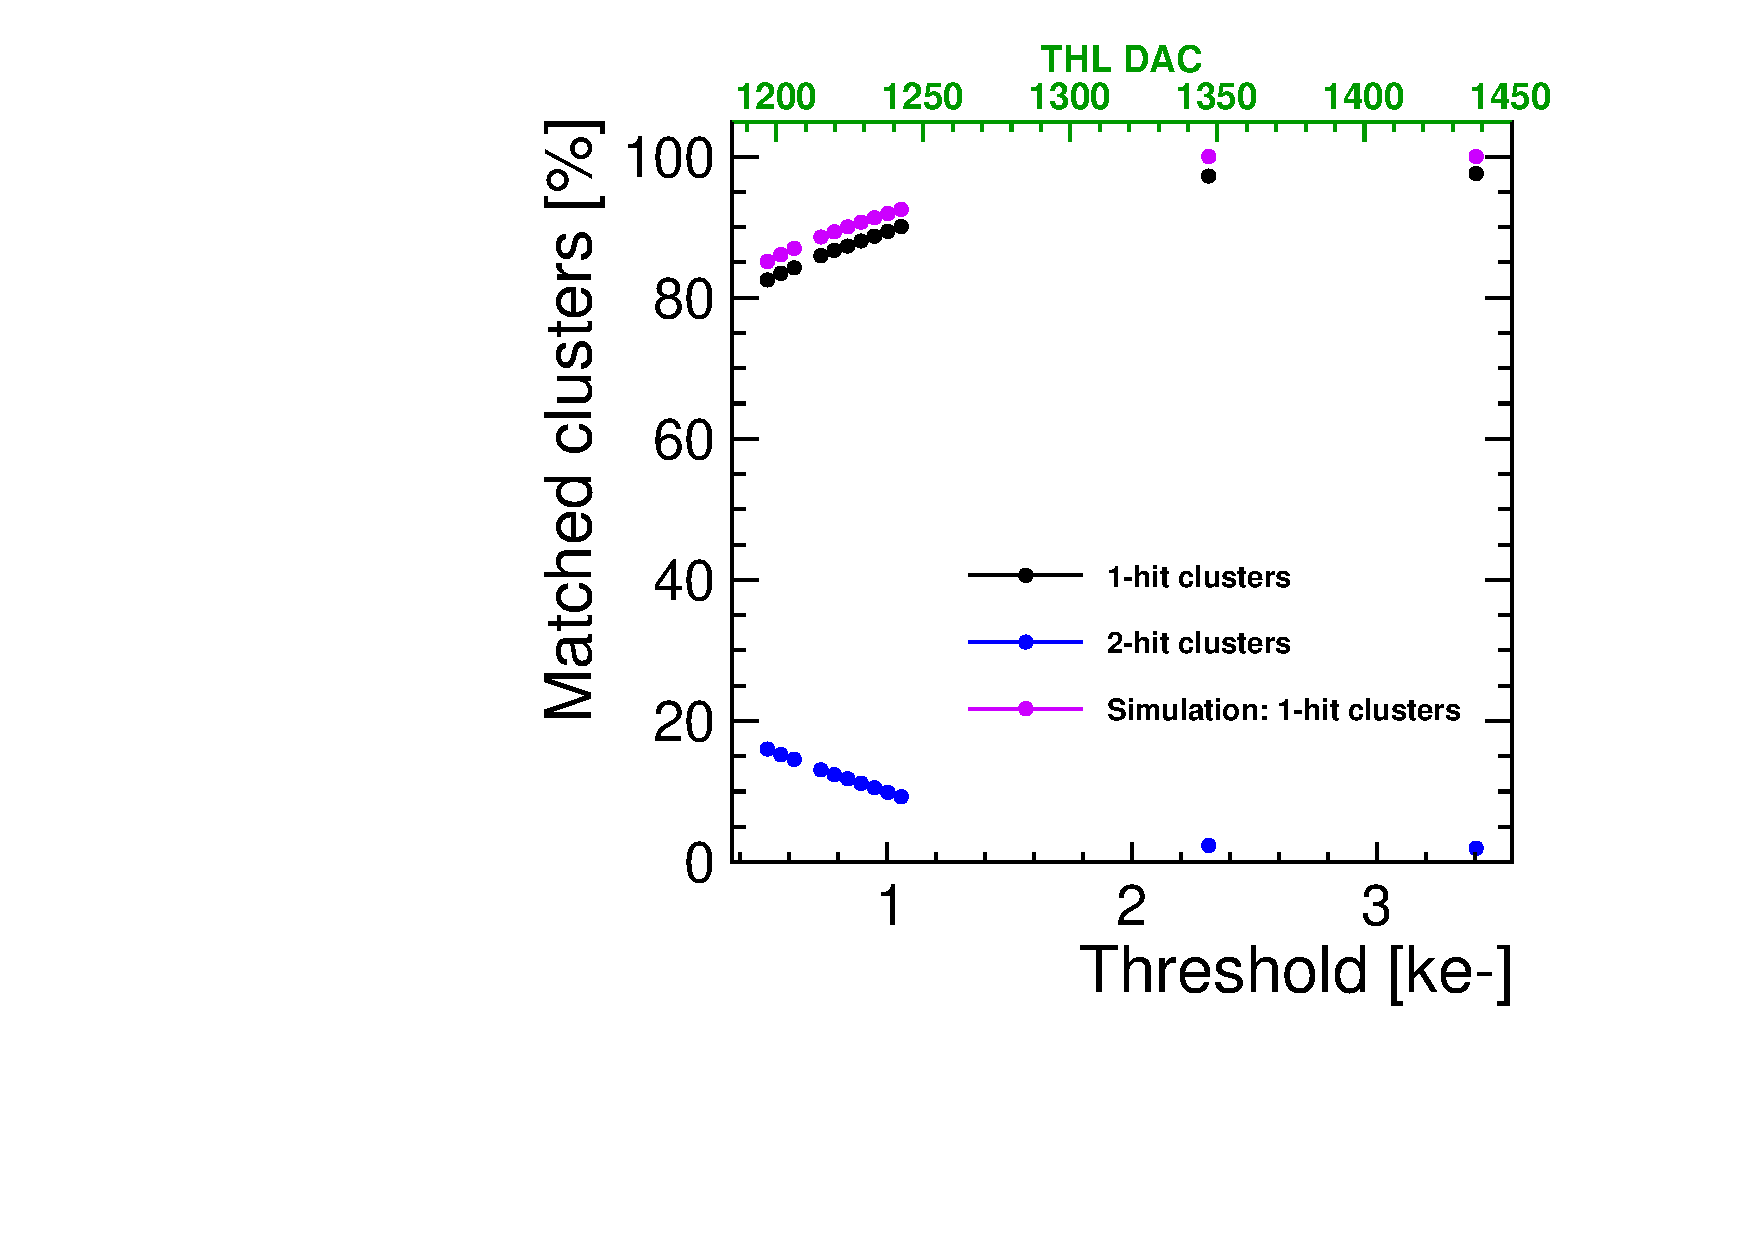
\includegraphics[width=\textwidth]{./figures/TestBeam/ThresholdScan_W0019_F07.pdf}
%%     \caption{}
%%   \end{subfigure} \hfill
%%   \begin{subfigure}[b]{0.45\textwidth}
%%     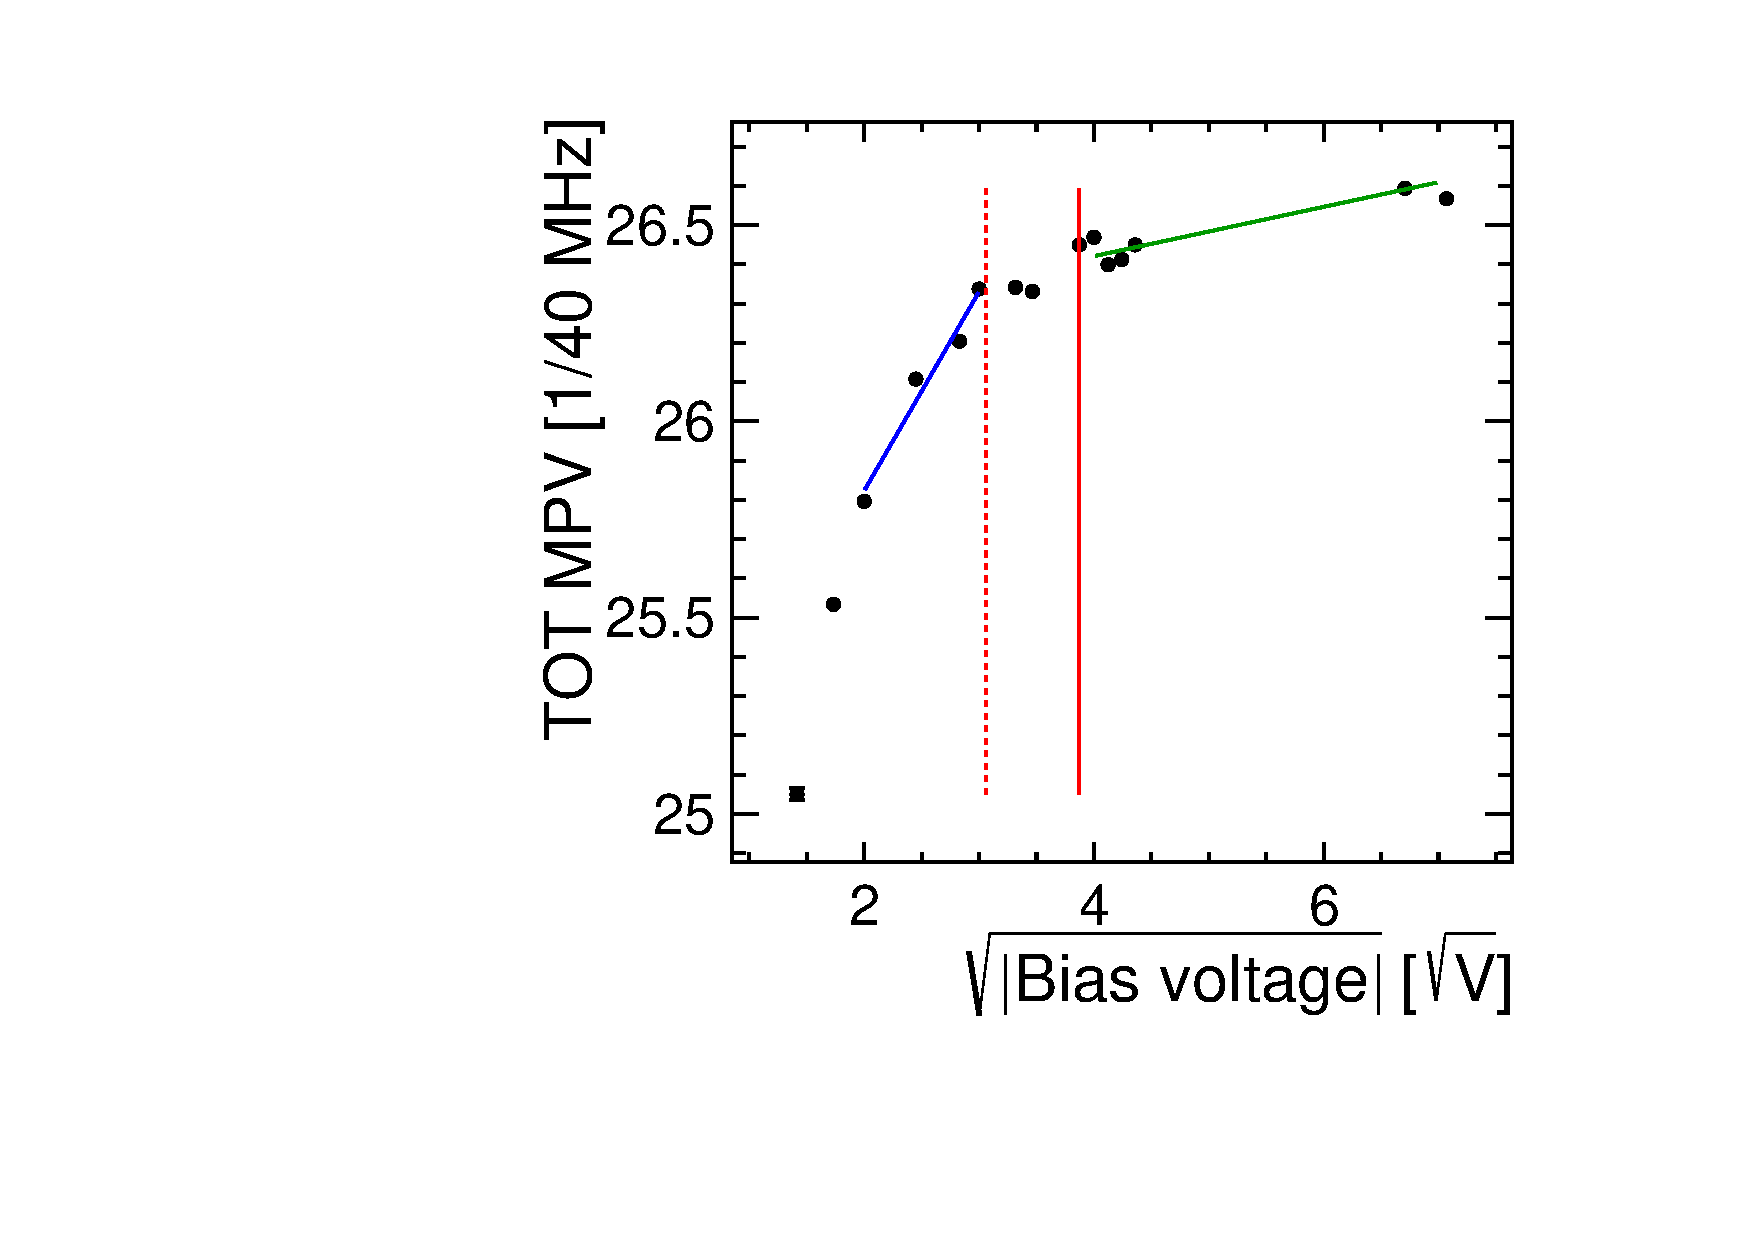
\includegraphics[width=\textwidth]{./figures/TestBeam/depletionVoltage_W0019_F07.pdf}
%%     \caption{}
%%   \end{subfigure}
%%   \caption{23-FGR (W19\_F7): bias and voltage scan.}
%%   \label{fig:Timepix3_THLscan_Vdep_F7}
%% \end{figure}

%% \begin{figure}[htbp] \centering
%%   \begin{subfigure}[b]{0.45\textwidth}
%%     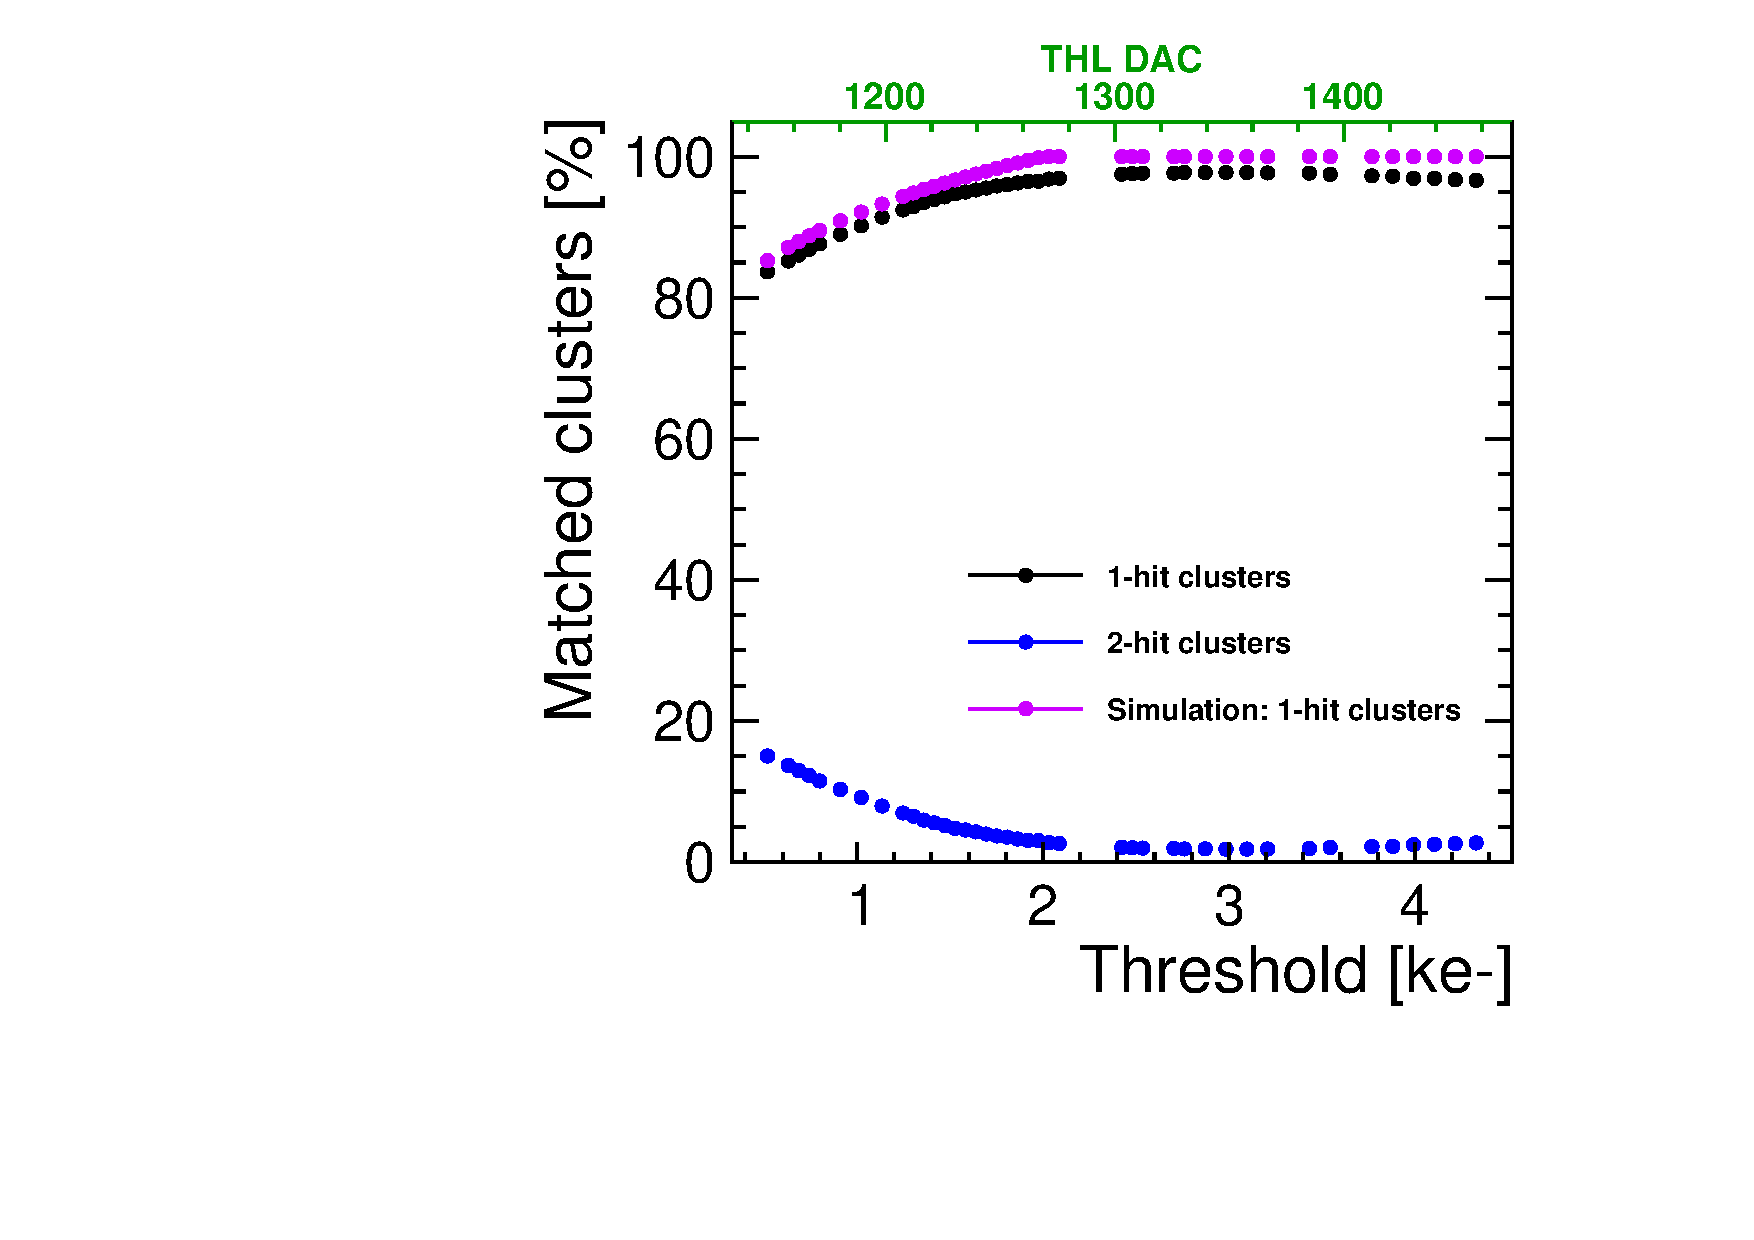
\includegraphics[width=\textwidth]{./figures/TestBeam/ThresholdScan_W0019_L08.pdf}
%%     \caption{}
%%   \end{subfigure} \hfill
%%   \begin{subfigure}[b]{0.45\textwidth}
%%     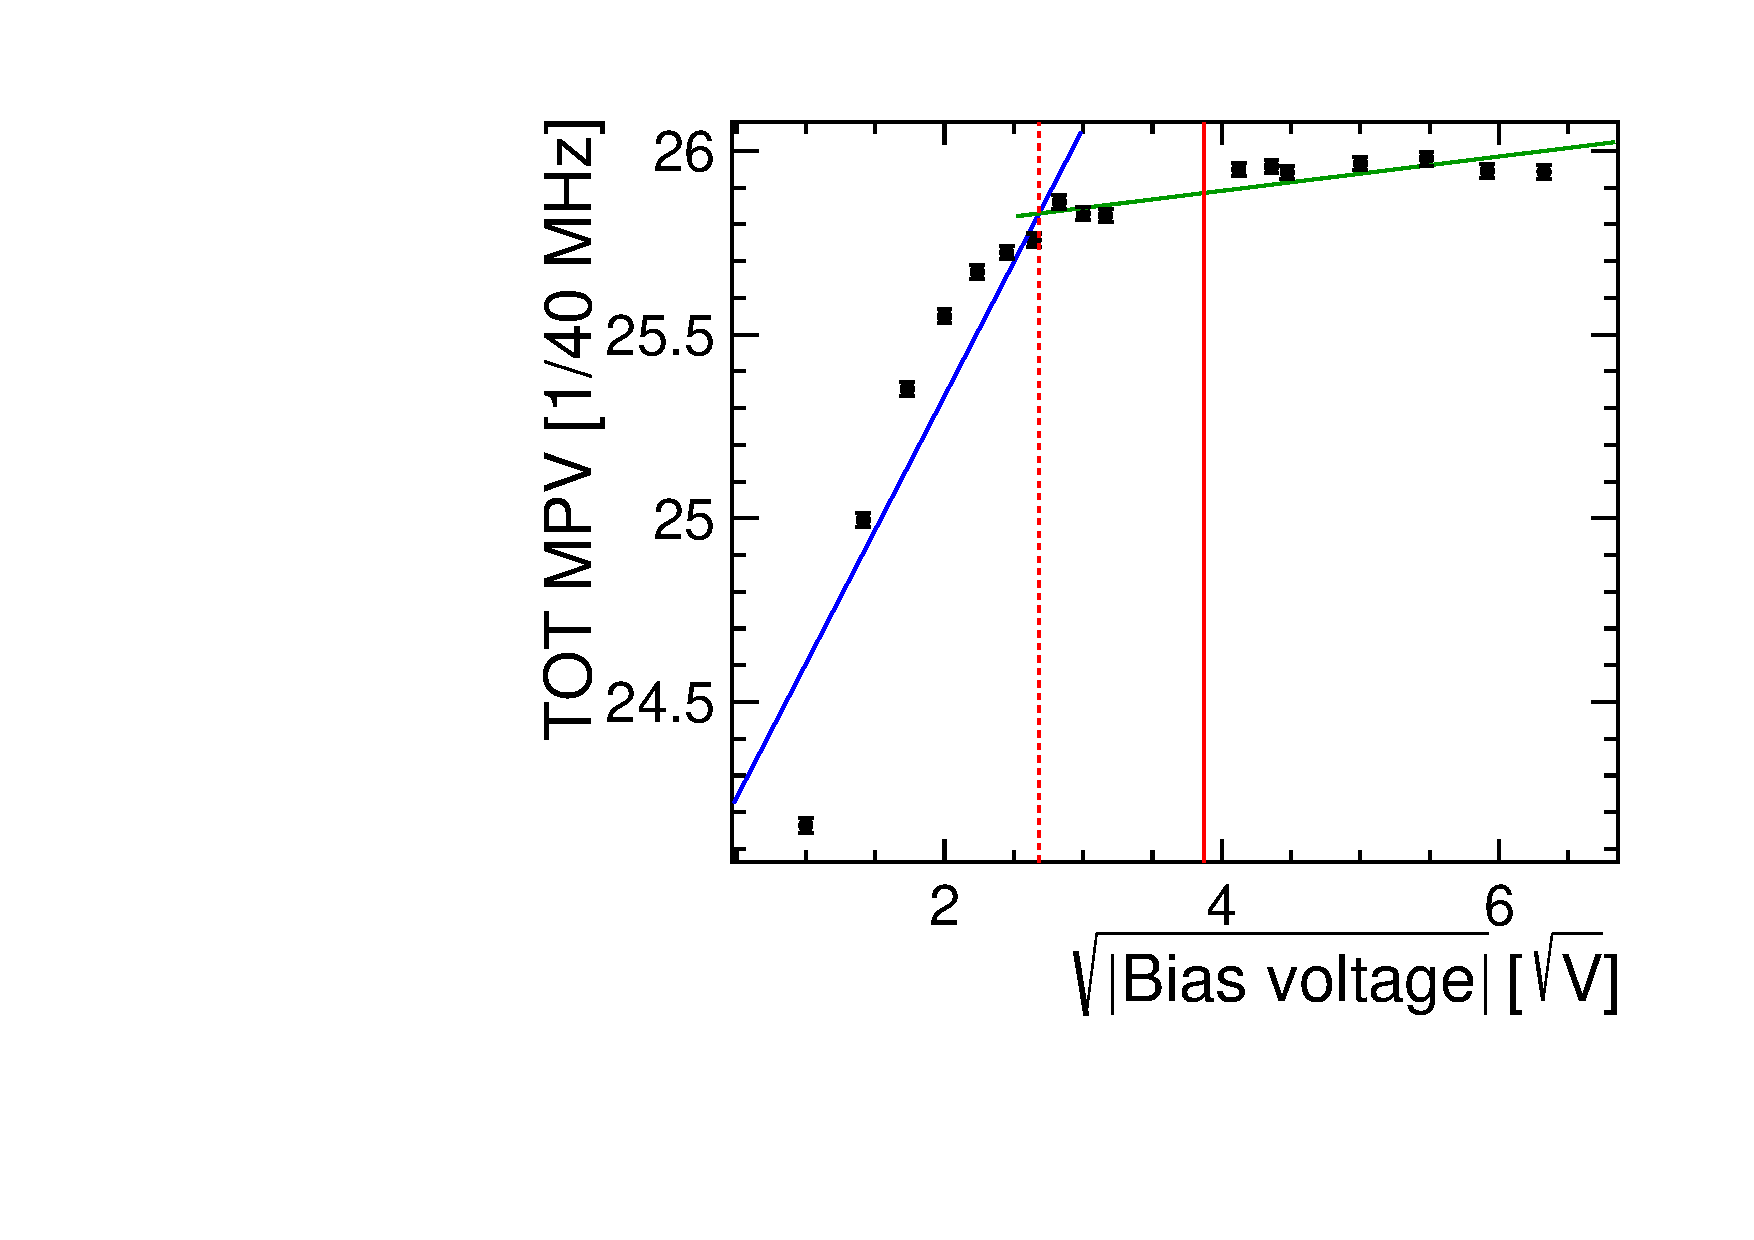
\includegraphics[width=\textwidth]{./figures/TestBeam/depletionVoltage_W0019_L08.pdf}
%%     \caption{}
%%   \end{subfigure}
%%   \caption{28-GNDGR (W19\_L8): bias and voltage scan.}
%%   \label{fig:Timepix3_THLscan_Vdep_L8}
%% \end{figure}


%% \begin{figure}[htbp] \centering
%%   \begin{subfigure}[b]{0.45\textwidth}
%%     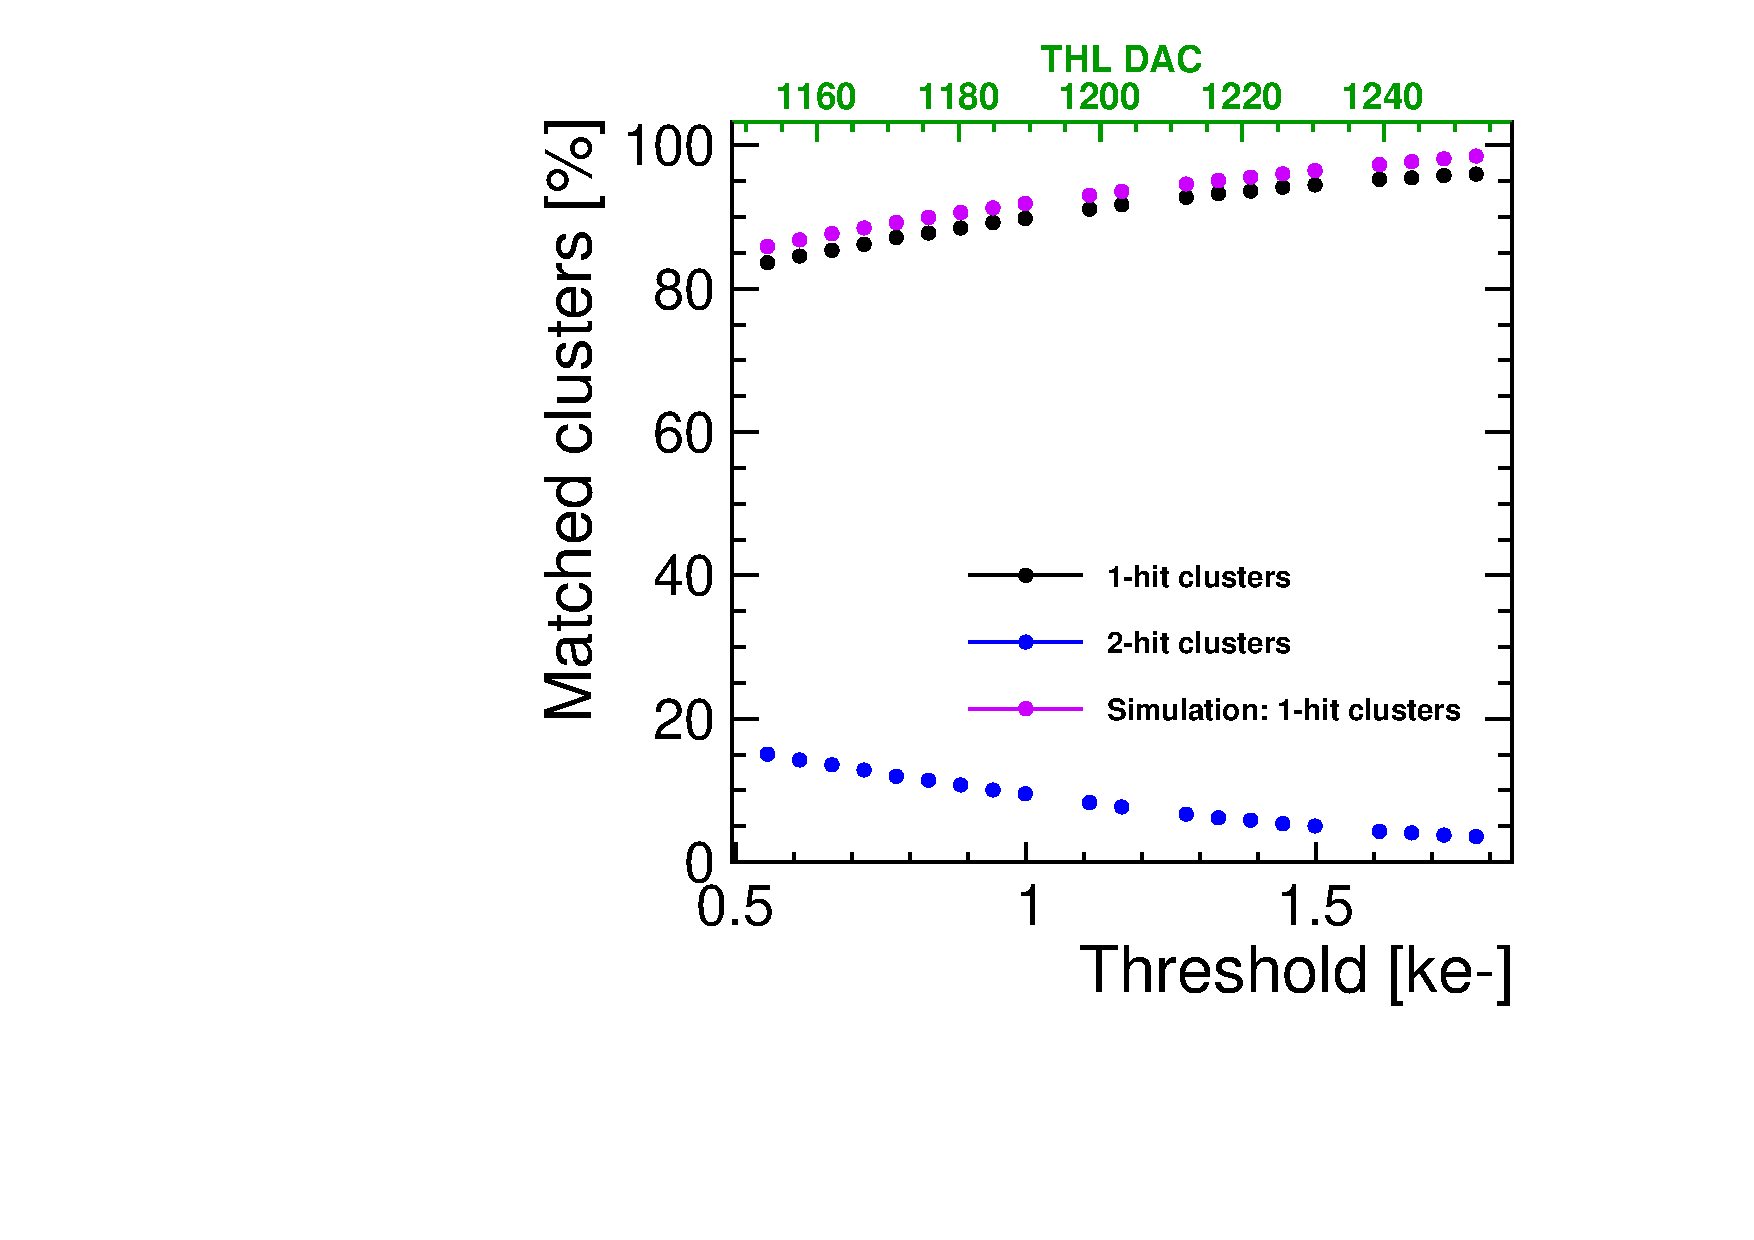
\includegraphics[width=\textwidth]{./figures/TestBeam/ThresholdScan_W0019_C07.pdf}
%%     \caption{}
%%   \end{subfigure} \hfill
%%   \begin{subfigure}[b]{0.45\textwidth}
%%     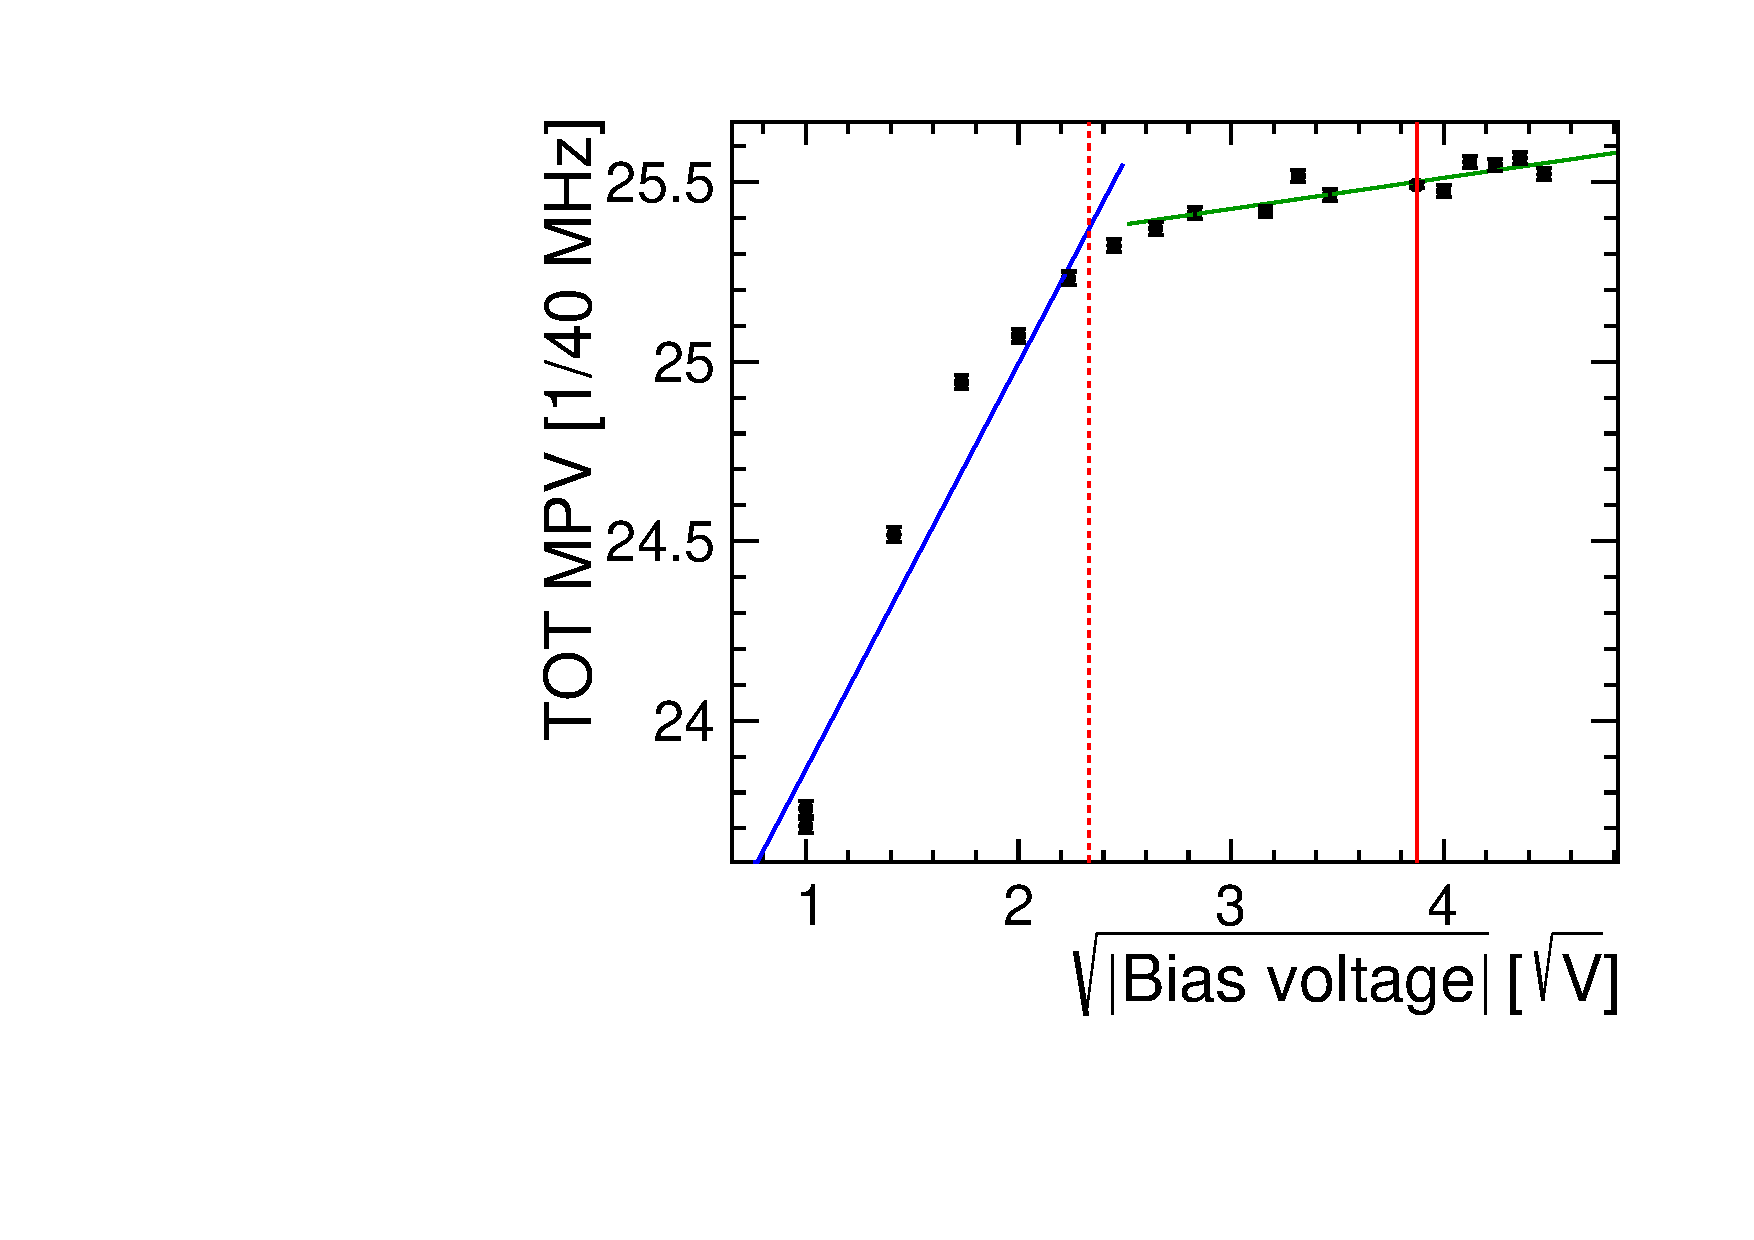
\includegraphics[width=\textwidth]{./figures/TestBeam/depletionVoltage_W0019_C07.pdf}
%%     \caption{}
%%   \end{subfigure}
%%   \caption{55-GNDGR (W19\_C7): bias and voltage scan.}
%%   \label{fig:Timepix3_THLscan_Vdep_C7}
%% \end{figure}

%% \begin{figure}[htbp] \centering
%%   \begin{subfigure}[b]{0.45\textwidth}
%%     \includegraphics[width=\textwidth]{./figures/TestBeam/ThresholdScan_W0005_E02.pdf}
%%     \caption{}
%%   \end{subfigure} \hfill
%%   \begin{subfigure}[b]{0.45\textwidth}
%%     \includegraphics[width=\textwidth]{./figures/TestBeam/depletionVoltage_W0005_E02.pdf}
%%     \caption{}
%%   \end{subfigure}
%%   \caption{55-GNDGR-100 (W5\_E2): bias and voltage scan.}
%%   \label{fig:Timepix3_THLscan_Vdep_E2}
%% \end{figure}


%% \begin{figure}[htbp] \centering
%%   \begin{subfigure}[b]{0.45\textwidth}
%%     \includegraphics[width=\textwidth]{./figures/TestBeam/ThresholdScan_W0005_F01.pdf}
%%     \caption{}
%%   \end{subfigure} \hfill
%%   \begin{subfigure}[b]{0.45\textwidth}
%%     \includegraphics[width=\textwidth]{./figures/TestBeam/depletionVoltage_W0005_F01.pdf}
%%     \caption{}
%%   \end{subfigure}
%%   \caption{55-GNDGR-150 (W5\_F1): bias and voltage scan.}
%%   \label{fig:Timepix3_THLscan_Vdep_F1}
%% \end{figure}




%% \begin{table}[htbp]
%%   \centering
%%   \caption{Measured depletion voltage for the assemblies described in
%%     \cref{tab:Timepix3Assemblies} and calculated by fitting the
%%     plateau and slope regions of TOT as a function of bias voltage.}
%%   \label{tab:depletionVoltage}
%%   \begin{tabular}{lcccc}
%%     \toprule
%%     Assembly & Thickness [\micron] & Sensor type & Nominal voltage [V] & Depletion voltage [V] \\
%%     \midrule
%%     20-NGR  & 50 & n-in-p & -15 & $<$-9.47 \\
%%     23-FGR & 50 & n-in-p & -15 & $<$-6.32 \\
%%     28-GNDGR & 50 & n-in-p & -15 & $<$-7.19\\
%%     55-GNDGR & 50 & n-in-p & -15 & $<$-5.43\\ \hline
%%     55-GNDGR-100 & 100 & n-in-p & -20 & -10.82 \\ \hline
%%     55-GNDGR-150 & 150 & n-in-p & -30 & -14.86 \\ \hline
%%     W2\_J5       & 300 & p-in-n & 100 & 63.23 \\ 
%%     \bottomrule
%%   \end{tabular}
%% \end{table}


%% \begin{table}[htbp]
%%   \centering
%%   \caption{Measured depletion voltage}
%%   \label{tab:depletionVoltage}
%%   \begin{tabular}{lcccc}
%%     \toprule
%%     Assembly & Thickness [\micron] & Sensor type & Nominal voltage [V] & Depletion voltage [V] \\
%%     \midrule
%%     20-NGR  & 50 & n-in-p & -15 & $<$-9.47 \\
%%     23-FGR & 50 & n-in-p & -15 & $<$-6.32 \\
%%     28-GNDGR & 50 & n-in-p & -15 & $<$-7.19\\
%%     55-GNDGR & 50 & n-in-p & -15 & $<$-5.43\\ \hline
%%     55-GNDGR-100 & 100 & n-in-p & -20 & -10.82 \\ \hline
%%     55-GNDGR-150 & 150 & n-in-p & -30 & -14.86 \\ \hline
%%     W2\_J5       & 300 & p-in-n & 100 & 63.23 \\ 
%%     \bottomrule
%%   \end{tabular}
%% \end{table}


%%%%\subsection{Resolution vs. thickness}
% \begin{figure}[htbp] \centering
%   \begin{subfigure}[b]{0.45\textwidth}
%     \includegraphics[width=\textwidth]{./figures/TestBeam/cluSize_vs_thickness.pdf}
%     \caption{}
%   \end{subfigure} \hfill
%   \begin{subfigure}[b]{0.45\textwidth}
%     \includegraphics[width=\textwidth]{./figures/TestBeam/residuals_vs_thickness.pdf}
%     \caption{}
%   \end{subfigure}
%   \caption{Cluster size and residuals vs. thickness (run 2003 for 300 um thick sensor was taken at 70 V).}
%   \label{fig:clusize_residuals_vs_thickness}
% \end{figure}


%% \begin{figure}[htbp] \centering
%%   \begin{subfigure}[b]{0.3\textwidth}
%%     \includegraphics[width=\textwidth]{figures/TestBeam/50micron_sizeX.pdf}
%%     \caption{}
%%   \end{subfigure} \hfill
%%   \begin{subfigure}[b]{0.3\textwidth}
%%     \includegraphics[width=\textwidth]{figures/TestBeam/50micron_resX.pdf}
%%     \caption{}
%%   \end{subfigure} \hfill
%%   \begin{subfigure}[b]{0.3\textwidth}
%%     \includegraphics[width=\textwidth]{figures/TestBeam/50micron_Edep.pdf}
%%     \caption{}
%%   \end{subfigure}
%%   \caption{For $50\,\micron$ thick sensor.}
%%   \label{fig:G4_simu_data_50micron}
%% \end{figure}

%% \begin{figure}[htbp] \centering
%%   \begin{subfigure}[b]{0.3\textwidth}
%%     \includegraphics[width=\textwidth]{figures/TestBeam/100micron_sizeX.pdf}
%%     \caption{}
%%   \end{subfigure} \hfill
%%   \begin{subfigure}[b]{0.3\textwidth}
%%     \includegraphics[width=\textwidth]{figures/TestBeam/100micron_resX.pdf}
%%     \caption{}
%%   \end{subfigure} \hfill
%%   \begin{subfigure}[b]{0.3\textwidth}
%%     \includegraphics[width=\textwidth]{figures/TestBeam/100micron_Edep.pdf}
%%     \caption{}
%%   \end{subfigure}
%%   \caption{For $100\,\micron$ thick sensor.}
%%   \label{fig:G4_simu_data_100micron}
%% \end{figure}

%% \begin{figure}[htbp] \centering
%%   \begin{subfigure}[b]{0.3\textwidth}
%%     \includegraphics[width=\textwidth]{figures/TestBeam/150micron_sizeX.pdf}
%%     \caption{}
%%   \end{subfigure} \hfill
%%   \begin{subfigure}[b]{0.3\textwidth}
%%     \includegraphics[width=\textwidth]{figures/TestBeam/150micron_resX.pdf}
%%     \caption{}
%%   \end{subfigure} \hfill
%%   \begin{subfigure}[b]{0.3\textwidth}
%%     \includegraphics[width=\textwidth]{figures/TestBeam/150micron_Edep.pdf}
%%     \caption{}
%%   \end{subfigure}
%%   \caption{For $150\,\micron$ thick sensor.}
%%   \label{fig:G4_simu_data_150micron}
%% \end{figure}


%%%%% CALIBRATION vs. GEANT4
% \cref{sec:testBeamDataCalibrated_vs_G4} compares the
% calibrated data with the \textsc{Geant4} energy deposition using the
% PAI physics list (c.f. \cref{sec:Silicon_Geant4}) for $50\,\micron$,
% $100\,\micron$ and $150\,\micron$ thick planar sensors. There is a
% good agreement in terms of the most probable value (MPV) and the
% full-width-at-half-maximum (FWHM) in both simulation and data.
% \begin{figure}[htbp] \centering
%   \begin{subfigure}[b]{0.33\textwidth}
%     \includegraphics[width=\textwidth]{./figures/Calibration/Edep_G4_W0019_G07.pdf}
%     \caption{55-GNDGR}
%   \end{subfigure} \hfill
%   \begin{subfigure}[b]{0.33\textwidth}
%     \includegraphics[width=\textwidth]{./figures/Calibration/Edep_G4_W0005_E02.pdf}
%     \caption{55-GNDGR-100}
%   \end{subfigure}\hfill
%   \begin{subfigure}[b]{0.33\textwidth}
%     \includegraphics[width=\textwidth]{./figures/Calibration/Edep_G4_W0005_F01.pdf}
%     \caption{55-GNDGR-150}
%   \end{subfigure}
%   \caption{Calibrated energy distribution of test beam data for
%     different assemblies. The pixel-by-pixel calibration is applied to
%     the data which is obtained using test pulses. \textsc{Geant4}
%     energy deposition is obtained using the PAI physics list.}
%   \label{sec:testBeamDataCalibrated_vs_G4}
% \end{figure}
